\chapter{Dominant topics}
With the three versions of my corpus (original, INL-normalized and VARD2-normalized), I continue my analysis. To build topic models with \texttt{gensim}, I have to take a few preliminary steps. In this chapter I will therefore first explain how a corpus needs to be prepared in order to perform topic modeling and how I have chosen the optimal settings. Afterwards, I will build the final topic models and discuss the results.

\section{Preparation of data and choosing settings}
At first, a corpus needs to be tokenized. This means that each text will be converted to a list with separate words, and that punctuation will be removed. Besides that, it is useful to filter \enquote{stop words} from the corpus. Stop words are the very common words in a corpus, which are in this case mostly function words such as \textit{ik} (personal pronoun), \textit{de} (preposition) and \textit{en} (conjunction). Content words, which have a more specific meaning, are often less frequent than function words. I created a list with the 150 most frequent words, using the Python package \texttt{nltk.FreqDist} after tokenization with \texttt{nltk.tokenize.word\_tokenize(language="dutch")}. I did this once for each version of my corpus. I checked each list manually and removed the function words from it (see Table~\ref{table:RemovedWords}). The three stop lists can be found in the appendix. I used the code below:\footnote{In this paragraph I show the code and results from the preprocess of the VARD2-normalized corpus. For building topic models from the other corpora, I used the same settings.}

\begin{lstlisting}
	import glob
	import nltk
	from utils import is_punct
	
	TOKENIZER = nltk.tokenize.word_tokenize
	CORPUS_PATH = "Corpus/VARDnormalized/varded50/*.txt"
	STOP_WORDS_PATH = "stoplists/stoplist_VARD2.txt"
	STOP_WORDS = [s.lower() for s in open(STOP_WORDS_PATH, "r", encoding="utf-8").read().splitlines()]
	
	remove_stopwords = lambda x: [word.lower() for word in x if word.lower() not in STOP_WORDS and not is_punct(word) and len(word) > 1]
	
	texts = glob.glob(CORPUS_PATH, recursive=False)
	tokenized_texts = [TOKENIZER(open(text, "r", encoding="utf-8").read(), language="dutch") for text in texts]
	tokenized_texts = [remove_stopwords(text) for text in tokenized_texts]
\end{lstlisting}

\noindent I added \texttt{len(word) > 1} to the function \texttt{remove\_stopwords} to make sure that no punctuation was left that for some reason was not included in the function \texttt{is\_punct}. After tokenization and punctuation removal, the song that was also discussed in the previous chapter, looked like this:

\begin{lstlisting}
["gulde", "zon", "maan", "mindre", "hemelvieren", "stargewelf", "versieren", "gods", "geboden", "gadeslaan", "felle", "noordewinden", "bruissend", "element", "stem", "zig", "laten", "binden", "roept", "god", "kent", "aards", "gezinde", "dwaze", "rot", "vroom", "geslagt", "verbolgen", "geneigd", "lust", "volgen", "durft", "zig", "uiten", "god", "welkers", "oordeel", "sta", "vrezen", "lighaam", "zinkt", "graf", "ziel", "verliest", "leggen", "leven", "af", "aartsverraders", "schrikt", "gods", "geduld", "hand", "tergen", "oog", "verbergen", "vreest", "vreest", "hemels", "strenge", "roe", "eenmaal", "genaken", "wrake", "traag", "schande", "maken","blixemvuur", "verslaan"]
\end{lstlisting}

\begin{table}[]
	\centering
	\begin{tabular}{ll}
		\toprule
		Corpus & removed words \\
		\midrule
		Original & \makecell{godt, heer, god, hert, leven, liefde, ziel, gods, heere, lief,\\min, heeren, godts, recht, mensch, menschen, lust}                                  \\
		INL      & \makecell{leven, heer, godt, hert, ziel, vreugde, hart, liefde, mens, tijd,\\gods, heere, kwaad, lief, zondaar, dag, dood, grond, eeuwig,\\kracht, wereld, hand} \\
		VARD2    & \makecell{god, gods, leven, hert, ziel, liefde, tijd, vreugd, here, geest,\\woord, lief, min, kwaad, zonden, heren, lof, hand, wereld,\\mens, mensen, recht} \\
		\bottomrule
	\end{tabular}
	\caption{Removed words from stop lists}
	\label{table:RemovedWords}
\end{table}

\noindent The two main inputs to a LDA topic model are \texttt{dictionary} and \texttt{corpus}. A dictionary is a commonly used \texttt{python} data type, containing \textit{key: value} pairs. Keys can be any immutable type, with the requirement that keys are unique within one dictionary. The keys of this dictionary are all unique tokens that exist in \texttt{tokenized\_texts}. The corresponding values are the number of times the words appear in \texttt{tokenized\_texts}. \texttt{gensim} creates a unique id for each word in a text. With \texttt{corpus}, a corpus is produced from \texttt{dictionary}, resulting in a mapping of [word\_id, word\_frequency].

\texttt{gensim} gives the opportunity to remove terms from the dictionary that appear too frequently or too infrequently in the corpus. This can be done with the functions \texttt{no\_below} and \texttt{no\_above}. The input for \texttt{no\_above} needs to be a number between 0 and 1: if \texttt{no\_above = 0.80}, terms that appear in more than 80\% of the documents are ignored. The input for \texttt{no\_below} needs to be an absolute number, corresponding with an actual number of documents: if \texttt{no\_below = 20}, terms that appear in less than 20 documents are ignored. The \texttt{no\_above} function can be seen as a tool to remove \enquote{corpus-specific stop words}. Since I already created a list with corpus-specific words, using the \texttt{no\_above} function is unnecessary. I therefore use \texttt{no\_above = 1}, implying that only tokens are removed that appear in more than 100\% of the documents, which, in fact, are zero tokens. Deciding what the right setting for \texttt{no\_below} is, is a bit of trial and error. I built three dictionaries (with \texttt{no\_below = 2}, \texttt{no\_below = 5} and \texttt{no\_below = 10}), using the following code:

\begin{lstlisting}
import gensim
from gensim import corpora
from gensim.corpora import Dictionary

NO_BELOW = 2 #and 5 and 10. minimum document frequency (absolute)
NO_ABOVE = 1 #maximum document frequency (fraction)

dictionary = Dictionary(tokenized_texts)
dictionary.filter_extremes(no_below=NO_BELOW, no_above=NO_ABOVE)
corpus = [dictionary.doc2bow(text) for text in tokenized_texts]
\end{lstlisting}

\noindent Table~\ref{table:DictSizesDifferentNB} contains the dictionary sizes at different settings for \texttt{no\_below}. It turns out that a rather big amount of tokens are discarded in all cases. At \texttt{no\_below = 2}, all tokens are removed that appear in only one text. This number of tokens is already quite high: 117,045. The number of discarded tokens only grows extensively when increasing \texttt{no\_below}. At \texttt{no\_below = 10}, only 19,912 tokens remain. This seems a really small number, but when we keep in mind that only those words are removed that appear in less than ten songs (out of a total number of 22,297 songs), this cut-off seems very reasonable.

\begin{table}[]
	\centering
	\begin{tabular}{llll}
		\toprule
		no\_below & 10 & 5 & 2 \\
		\midrule
		Discarded tokens & 174,247                & 160,705                & 117,045                \\
		Kept tokens      & 19,912                 & 33,454                 & 77,114          \\
		\bottomrule      
	\end{tabular}
	\caption{Dictionary sizes at different no\_below's}
	\label{table:DictSizesDifferentNB}
\end{table}

To make more sense of these numbers, I built a topic model for each setting of \texttt{no\_below} and compared the coherence score of each topic model.  The topic coherence provides a measure to judge how good a given topic model is. The output is a number between 0 and 1. The higher this number, the better the topic model. For the time being, I let the model create 50 topics. To build the topic model and to compute the coherence score, I used the following code:

\begin{lstlisting}
from gensim.models import CoherenceModel
from gensim.models.wrappers import LdaMallet

N_TOPICS = 50
ITERATIONS = 2000
OPTIMIZE_INTERVAL = 20
EVAL_EVERY = 3 #for regular LDA
N_WORKERS = 3 #number of CPU'S for multiprocessing

lda = LdaMallet("/Users/alielassche/applications/mallet/bin/mallet", corpus=corpus, id2word=dictionary, num_topics=N_TOPICS, iterations=ITERATIONS, workers=N_WORKERS, optimize_interval=OPTIMIZE_INTERVAL)

# Compute Coherence score
coherence_model_ldamallet = CoherenceModel(model=lda, texts=tokenized_texts, dictionary=dictionary, coherence="c_v")
coherence_ldamallet = coherence_model_ldamallet.get_coherence()
\end{lstlisting}

\noindent The results are stored in Table~\ref{table:CSDiffNB}. It turns out that the topic model made with \texttt{no\_below = 2} has the highest coherence score. Therefore I continue with that parameter setting.

\begin{table}[]
	\centering
	\begin{tabular}{ll}
		\toprule
		no\_below & Coherence score  \\
		\midrule
		2 & 0.50571         \\
		5 & 0.49573     \\
		10 & 0.49014 \\
		\bottomrule      
	\end{tabular}
	\caption{Coherence score at different no\_below's}
	\label{table:CSDiffNB}
\end{table}

The next step is to choose the number of topics. Since this parameter can highly influence the results, I use the coherence score here as well. With the code below, I calculate the coherence score for 10 topic models with different values for \texttt{num\_topics}, in the range 10:100.

\begin{lstlisting}
def compute_coherence_values(dictionary, corpus, texts, limit, start=2, step=3):

	coherence_values = []
	model_list = []
	for num_topics in range(start, limit, step):
	model = gensim.models.wrappers.LdaMallet
	("/Users/alielassche/applications/mallet/bin/mallet", corpus=corpus, num_topics=num_topics, id2word=dictionary, iterations=ITERATIONS,  
	workers=N_WORKERS, optimize_interval=OPTIMIZE_INTERVAL)
	model_list.append(model)
	coherencemodel = CoherenceModel(model=model, texts=tokenized_texts, dictionary=dictionary, coherence="c_v")
	coherence_values.append(coherencemodel.get_coherence())
	
	return model_list, coherence_values
	
	# model_list: List of LDA topic models
	# coherence_values: Coherence values corresponding to the LDA model with respective number of topics
	
model_list, coherence_values = compute_coherence_values(dictionary=dictionary, corpus=corpus, texts=tokenized_texts, start=10, limit=110, step=10)
\end{lstlisting}

\begin{figure}[hbt!]
	\centering
	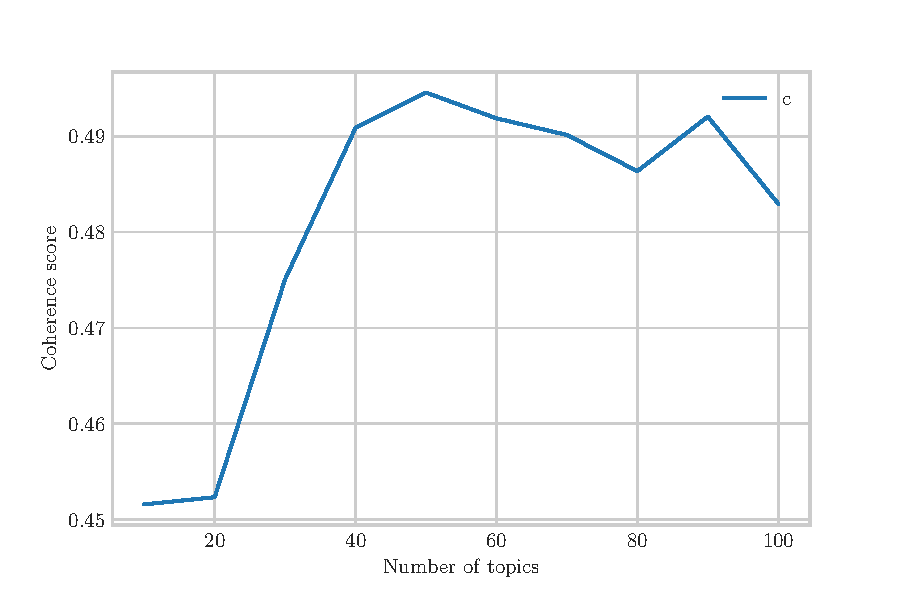
\includegraphics[scale=0.9]{coherence_values_2_10_100}
	\caption{Choosing an optimal number of topics with coherence scores}
	\label{fig:ChoosingTopicsWithCS}
\end{figure}

\noindent The results are plotted in Figure~\ref{fig:ChoosingTopicsWithCS}. The highest coherence score is obtained at \texttt{num\_topics = 50}. I therefore decided to build the final topic models using this setting. 

\section{Building the final topic models}
I built the final topic models for the three versions of my corpus with the following code:

\begin{lstlisting}
NO_BELOW = 2 #minimum document frequency
NO_ABOVE = 1 #maximum document frequency

N_TOPICS = 50
ITERATIONS = 2000
OPTIMIZE_INTERVAL = 20
EVAL_EVERY = 3 # for regular LDA 
N_WORKERS = 3 # number of CPU'S for multiprocessing

lda = LdaMallet("/Users/alielassche/applications/mallet/bin/mallet", 
corpus=corpus, id2word=dictionary, num_topics=N_TOPICS, iterations=ITERATIONS, workers=N_WORKERS, optimize_interval=OPTIMIZE_INTERVAL)
\end{lstlisting}

\noindent The most basic and important output of the function \texttt{LdaMallet} is two dataframes: one with the keys of a topic model, the other one with the composition. The dataframe \texttt{keys} contains 50 rows, for each topic one, and 2 columns: one for the topic number, the other one for the words that form a specific topic. The dataframe \texttt{composition} contains as many rows as there are texts in the corpus: in this case 22,297. The columns are numbered from 0 to 49, corresponding with the numbers of the topics from \texttt{keys}. The cells from each row contain the composition of the 50 topics in that text. The higher a value, the more dominant a topic is in a text. Other characteristics of the model, the topics or the texts can be obtained, but I will discuss that in more detail below, where I analyze the results of \texttt{LdaMallet} by the version of the corpus.

\subsection{Original corpus}
The dictionary that was built from the original corpus, contained at first 218,027 unique tokens, but after discarding 127,936 tokens (the number of tokens with a value of \texttt{1} in the dictionary, a result of the setting \texttt{no\_below = 2}), 90,091 tokens remained. I let the tool build 50 topics from this corpus and dictionary. The coherence score of the model was 0.5097. All topics with their corresponding words can be find in the appendix, but the most self-explanatory topics I show in some word clouds in the Figures~\ref{fig:topic3Original} to~\ref{fig:topic49Original}. I have to assign a word to each topic, with which the subject of the topic can be described. I assigned the subject \textit{love and sadness} to topic 3, which is pictured in Figure~\ref{fig:topic3Original}, because of the presence of positive words such as \enquote{lief}, \enquote{lieve}, \enquote{min} and \enquote{schoone} on the one hand and negative words as \enquote{smert}, \enquote{tranen}, \enquote{verdriet} and \enquote{pijn} on the other hand. This topic differs from another love-topic, topic 49 (Figure~\ref{fig:topic49Original}), in such way that almost all words in this topic are positive words: \enquote{hert}, \enquote{zoet}, \enquote{min}, \enquote{vreugd} and \enquote{lief}. I assign the subject \textit{love \& happiness} to this topic.

\begin{figure}
	\begin{minipage}[c]{0.48\linewidth}
		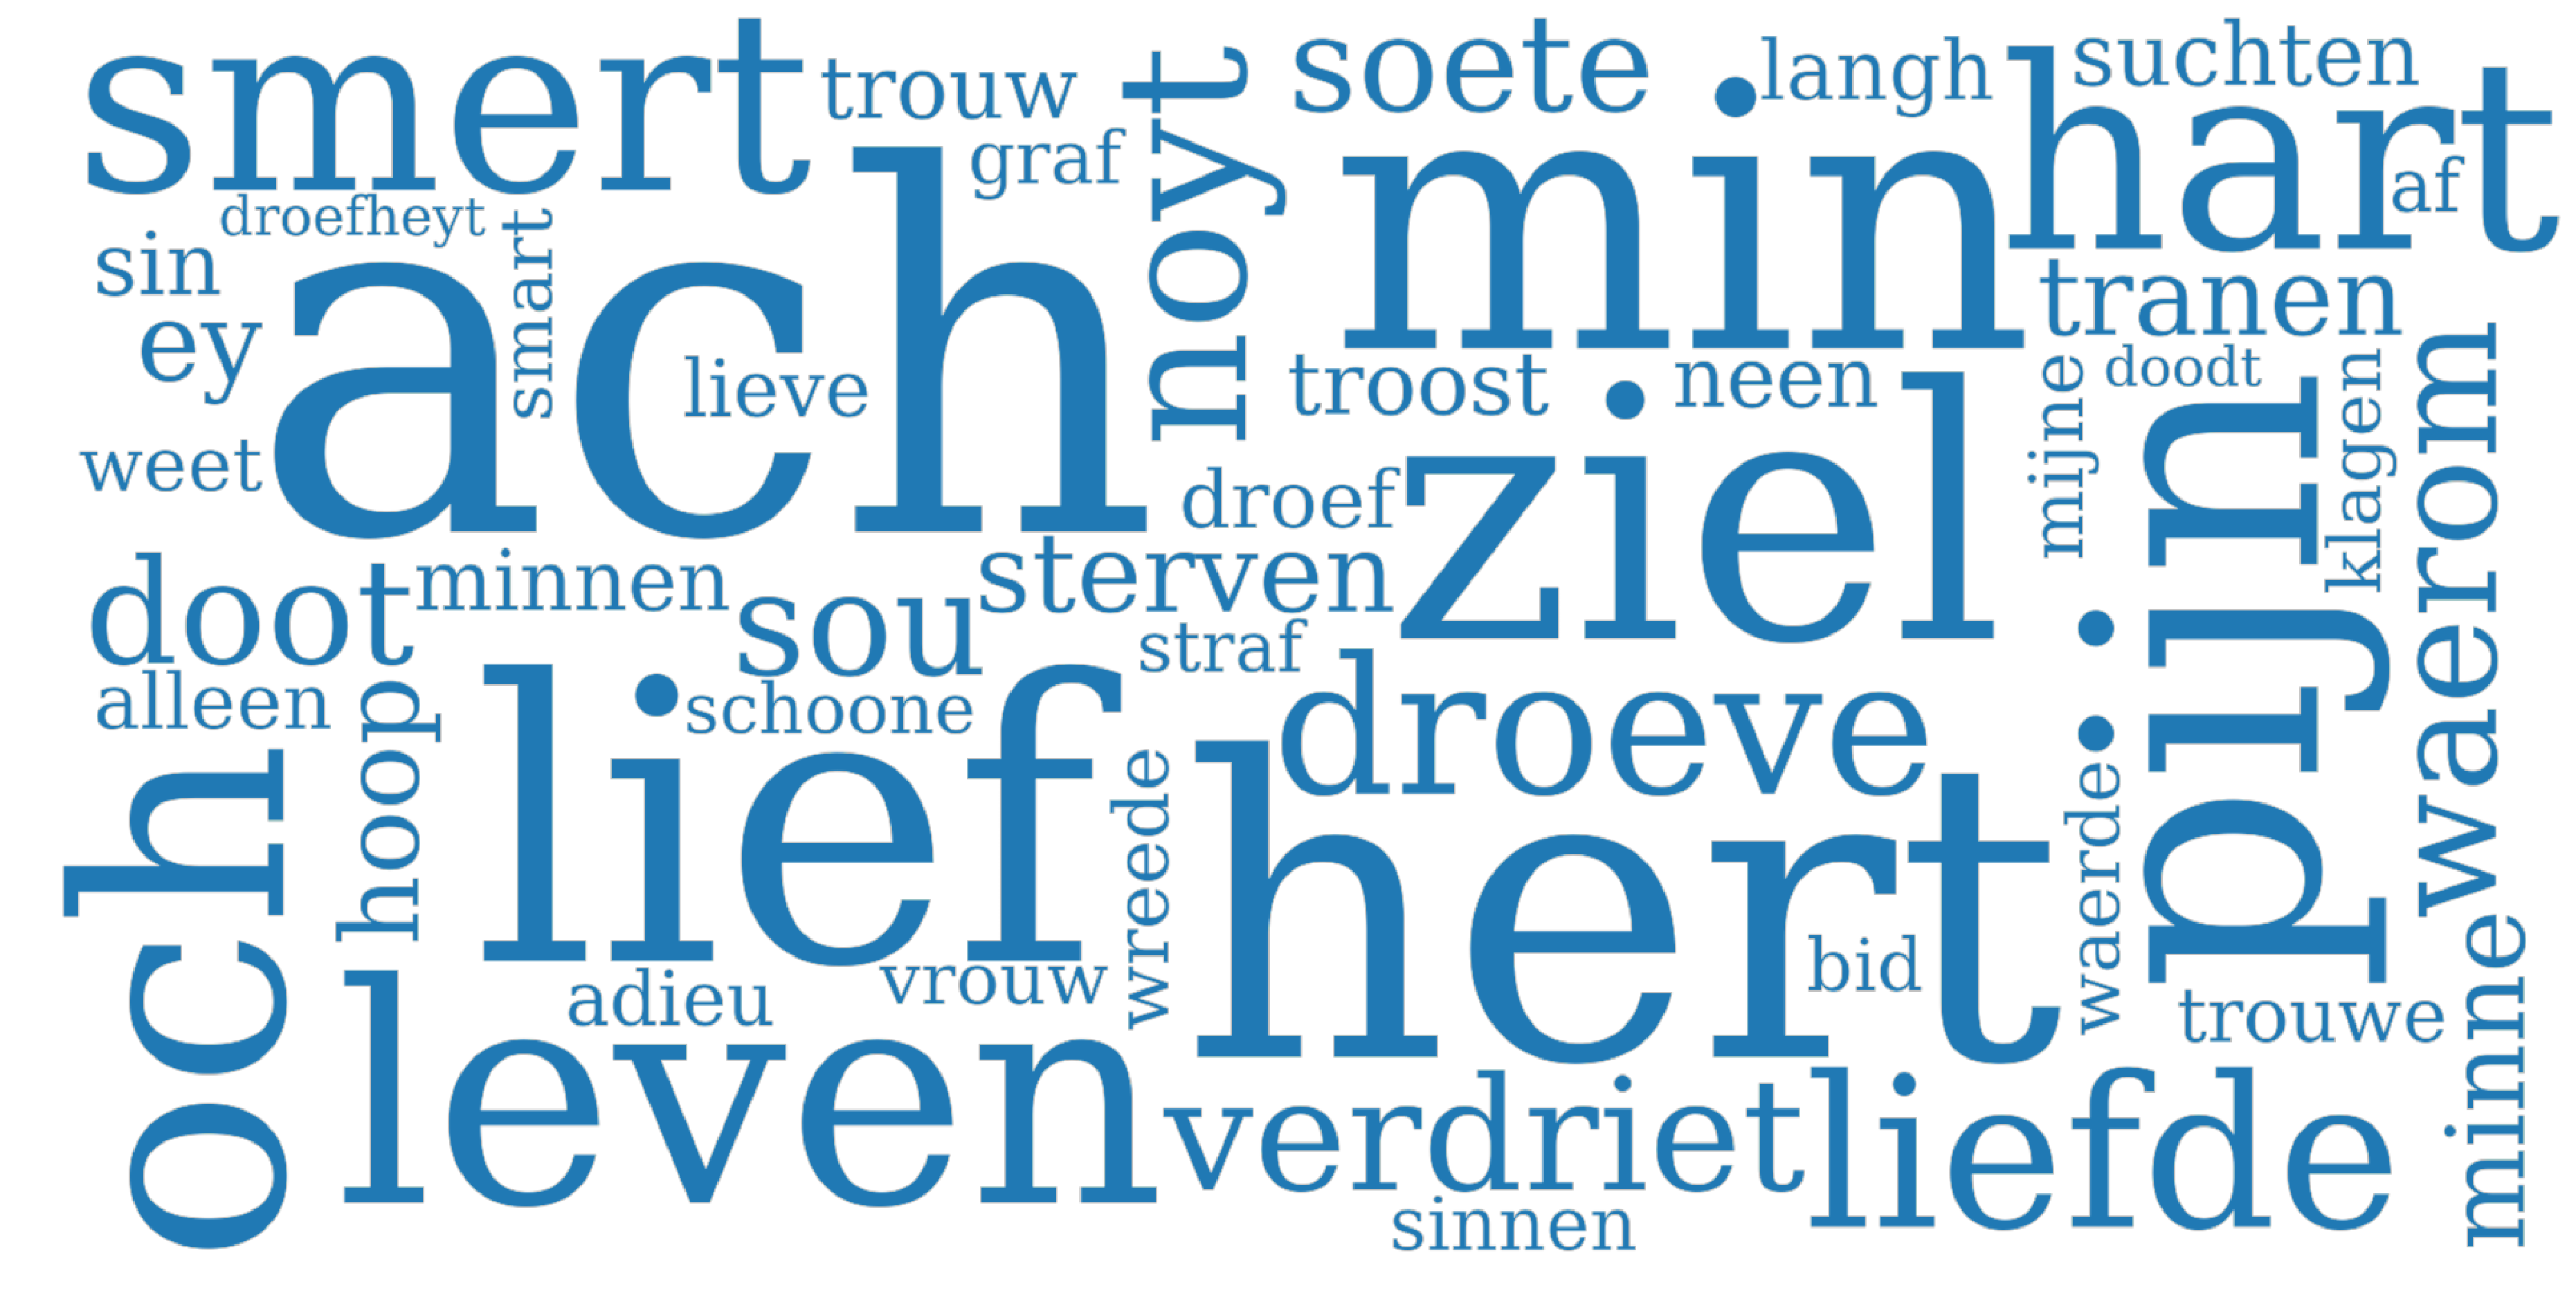
\includegraphics[width=\linewidth]{original_topic3}
		\caption{\textit{love \& sadness} (3)}
		\label{fig:topic3Original}
		\vspace{4ex}
	\end{minipage}%%
	\begin{minipage}[c]{0.48\linewidth}
		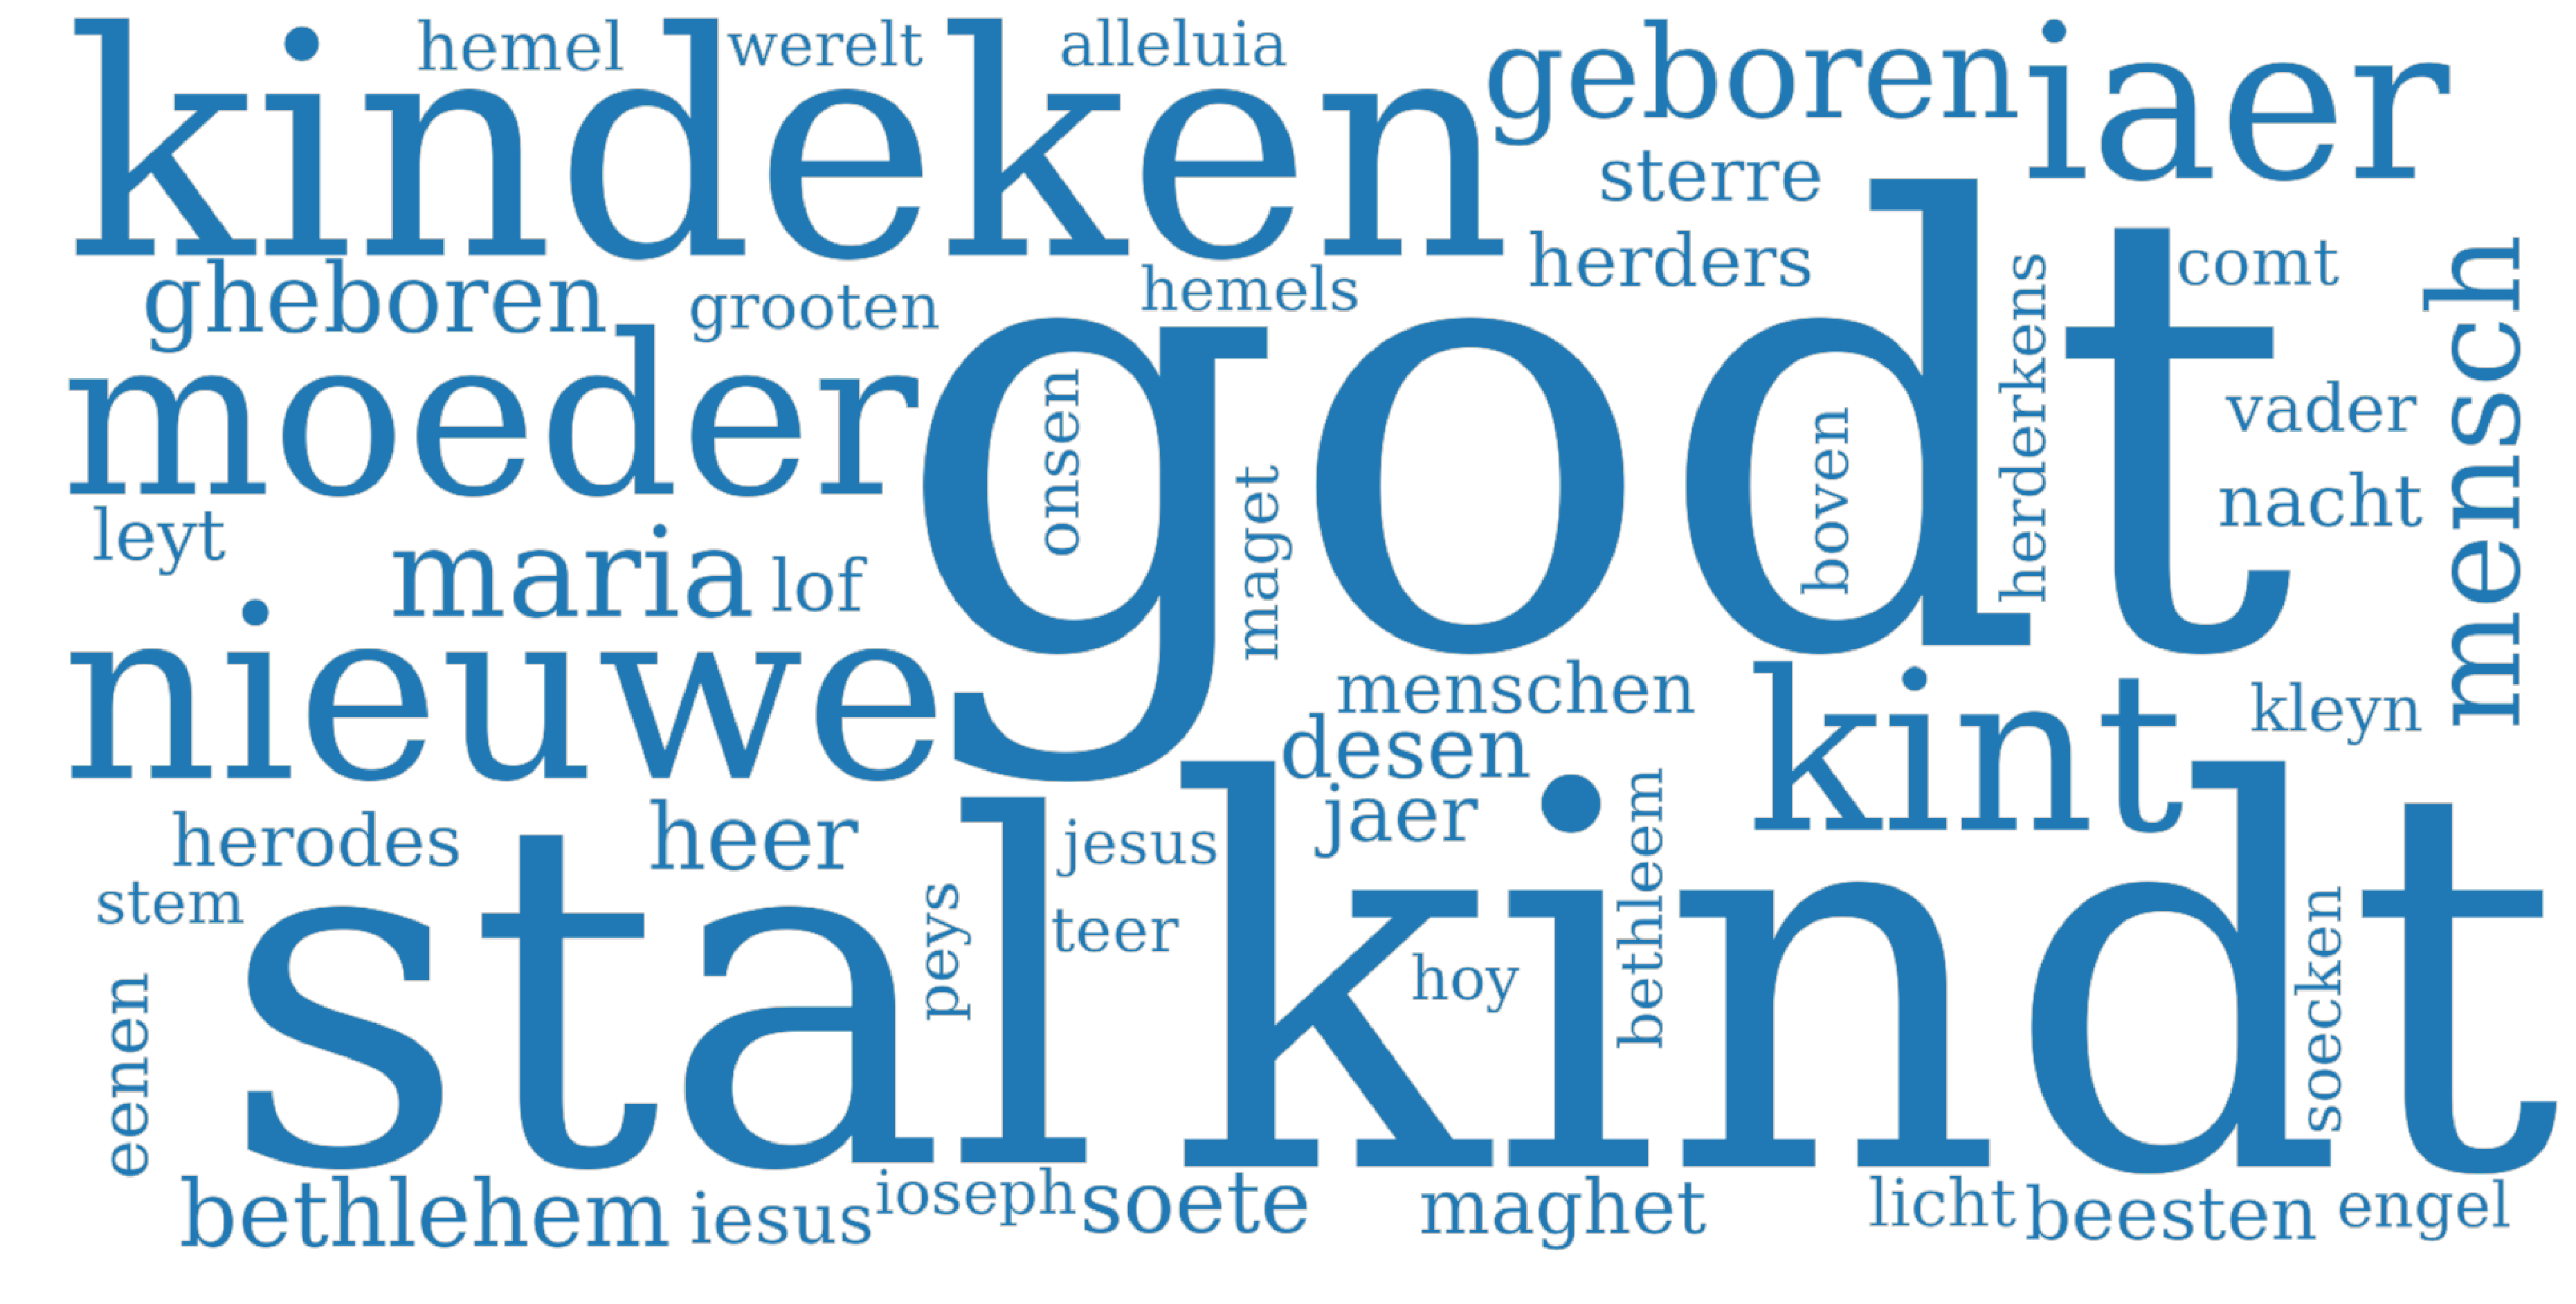
\includegraphics[width=\linewidth]{original_topic7}
		\caption{\textit{Christmas} (7)}
		\label{fig:topic7Original}
		\vspace{4ex}
	\end{minipage}%%
	\hfill
	\begin{minipage}[c]{0.48\linewidth}
		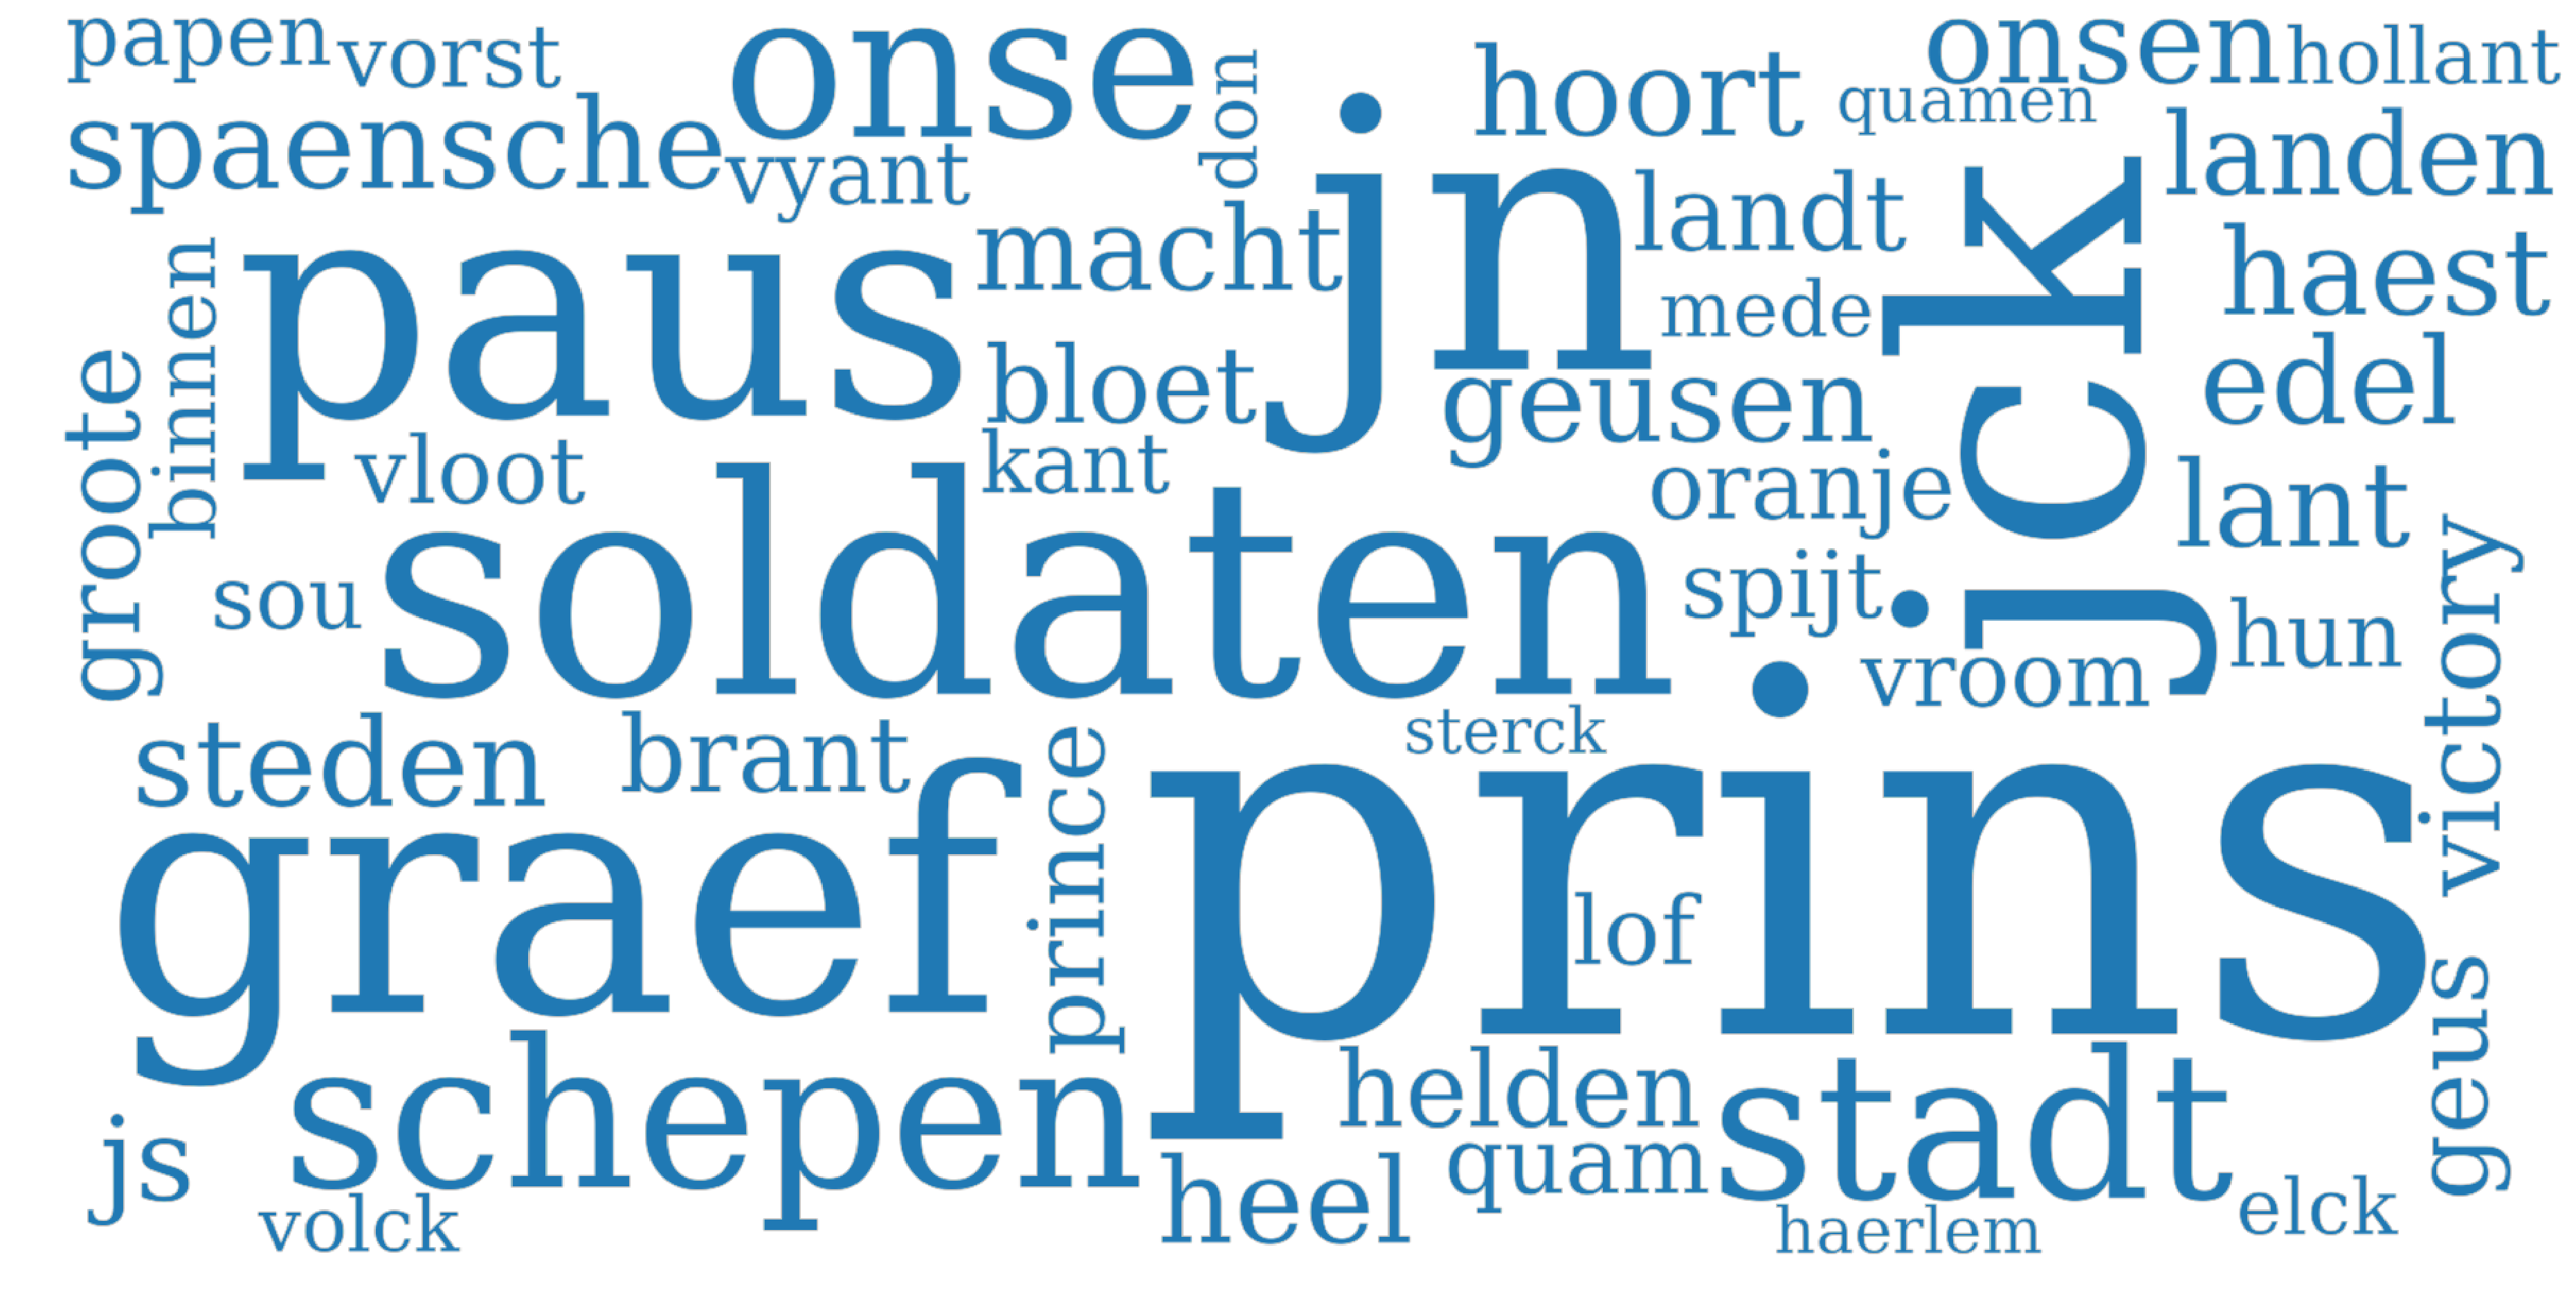
\includegraphics[width=\linewidth]{original_topic10}
		\caption{\textit{nation \& country} (10)}
		\label{fig:topic10Original}
		\vspace{4ex}
	\end{minipage}%%
	\begin{minipage}[c]{0.48\linewidth}
		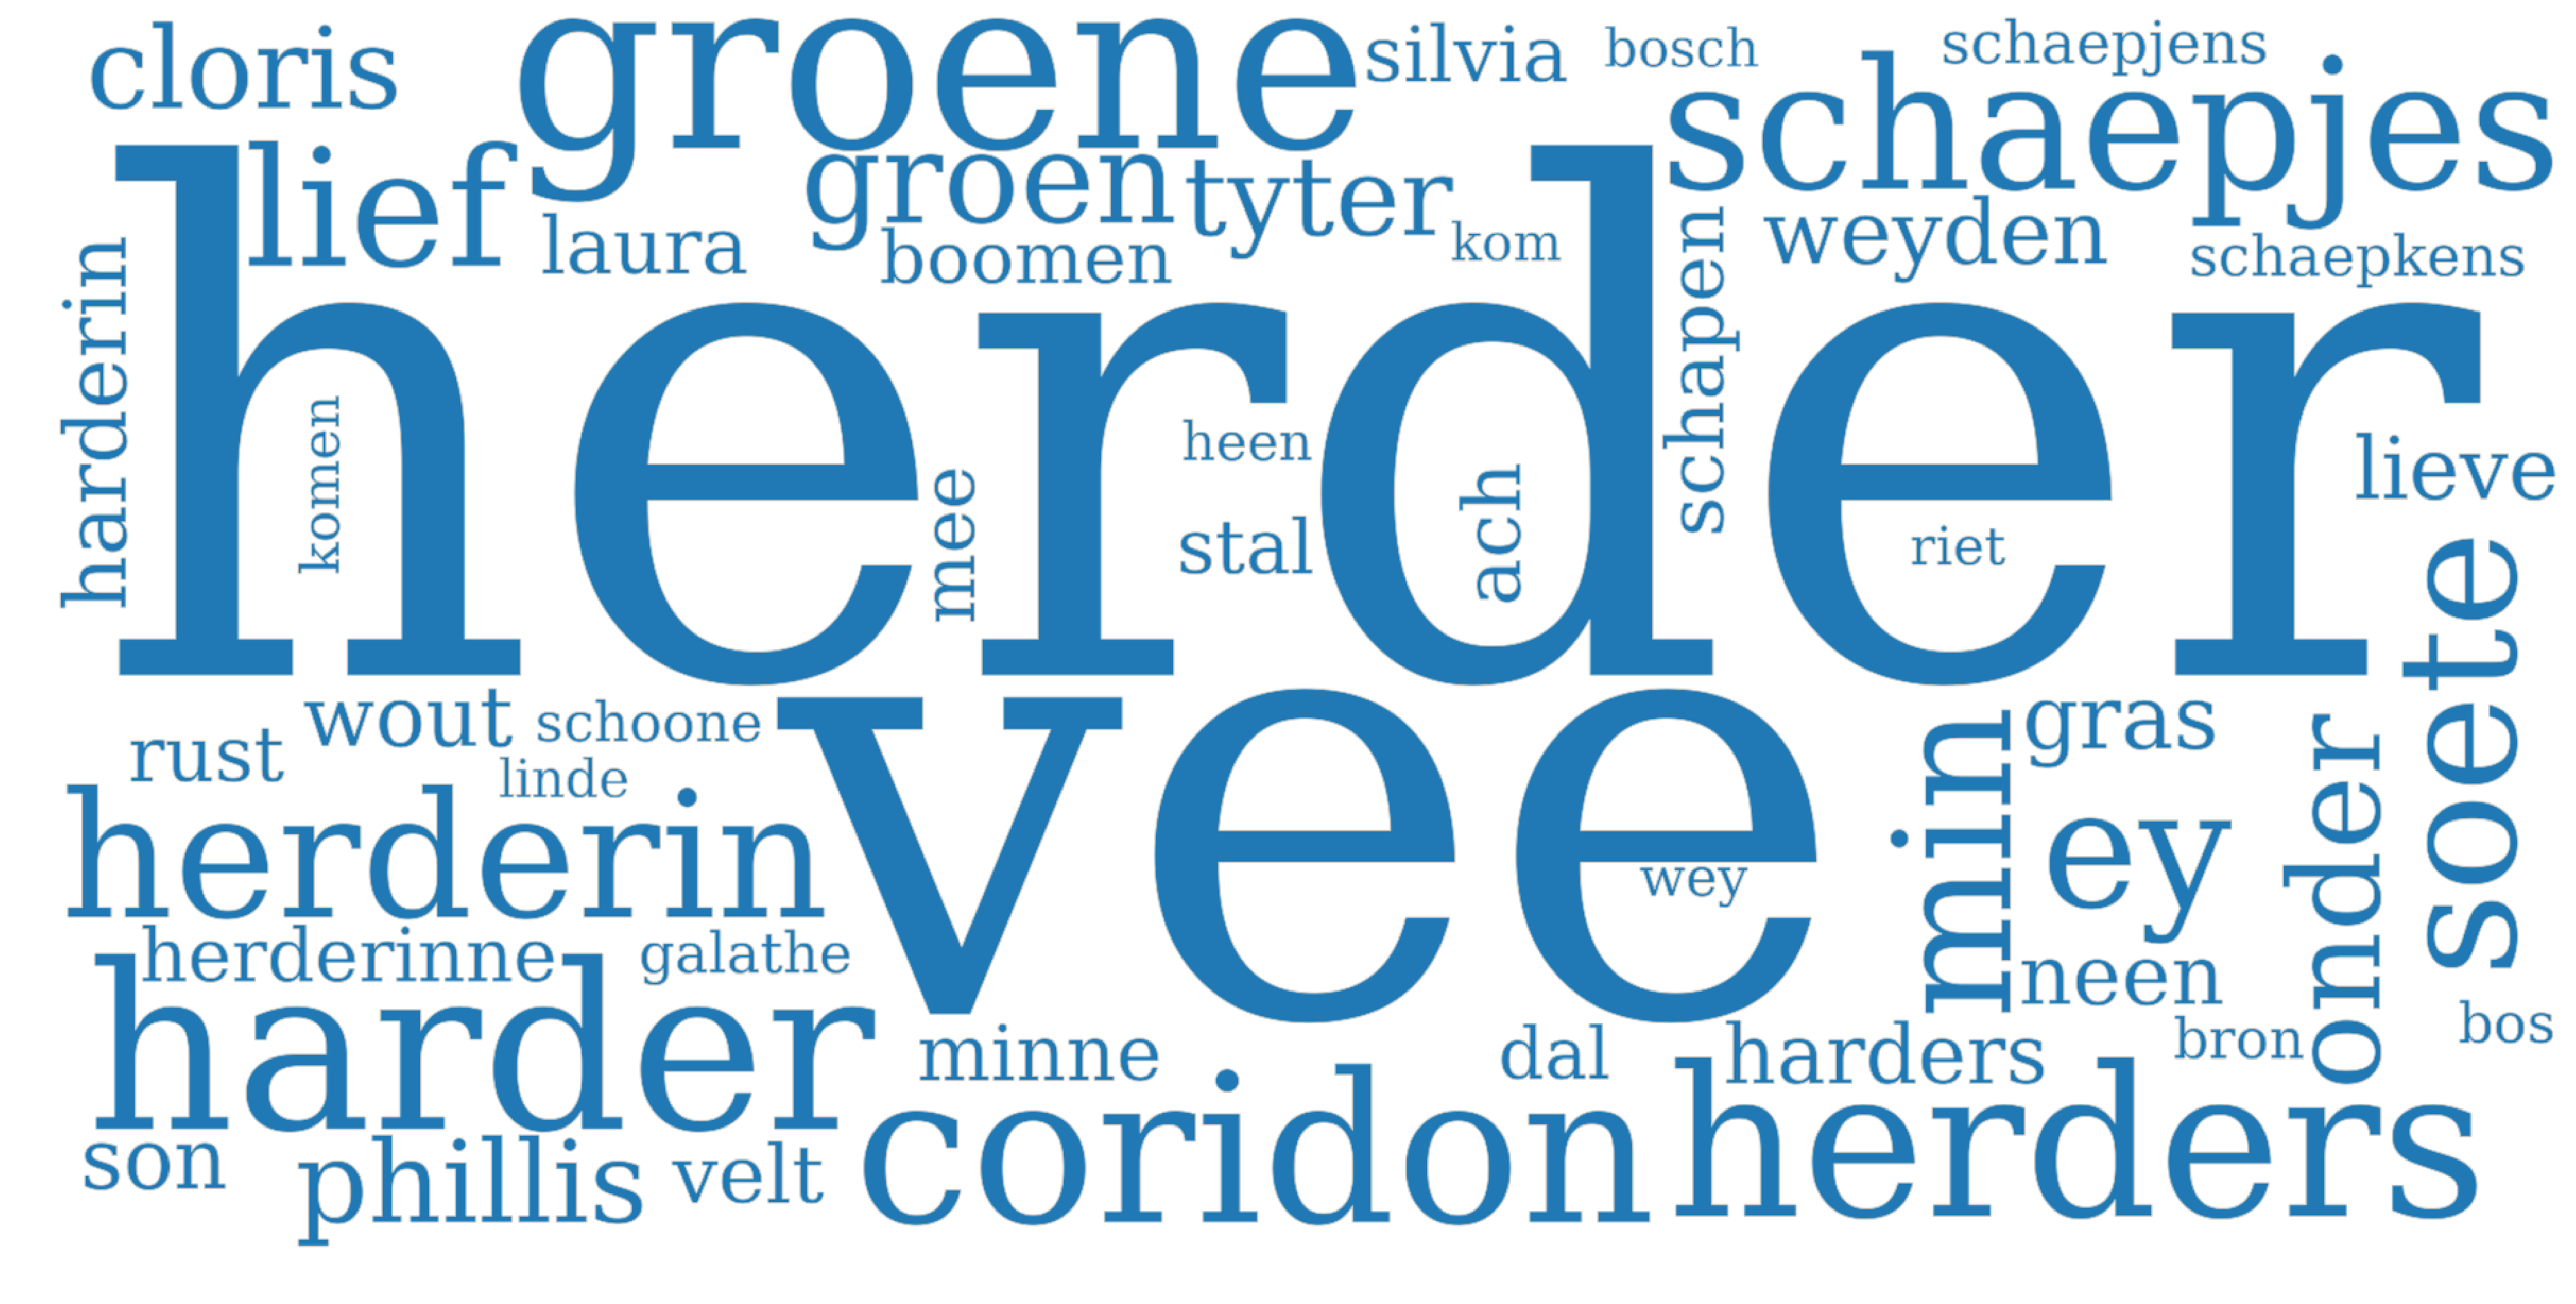
\includegraphics[width=\linewidth]{original_topic12}
		\caption{\textit{bucolic songs} (12)}
		\label{fig:topic12Original}
		\vspace{4ex}
	\end{minipage}%%
	\hfill
	\begin{minipage}[c]{0.48\linewidth}
		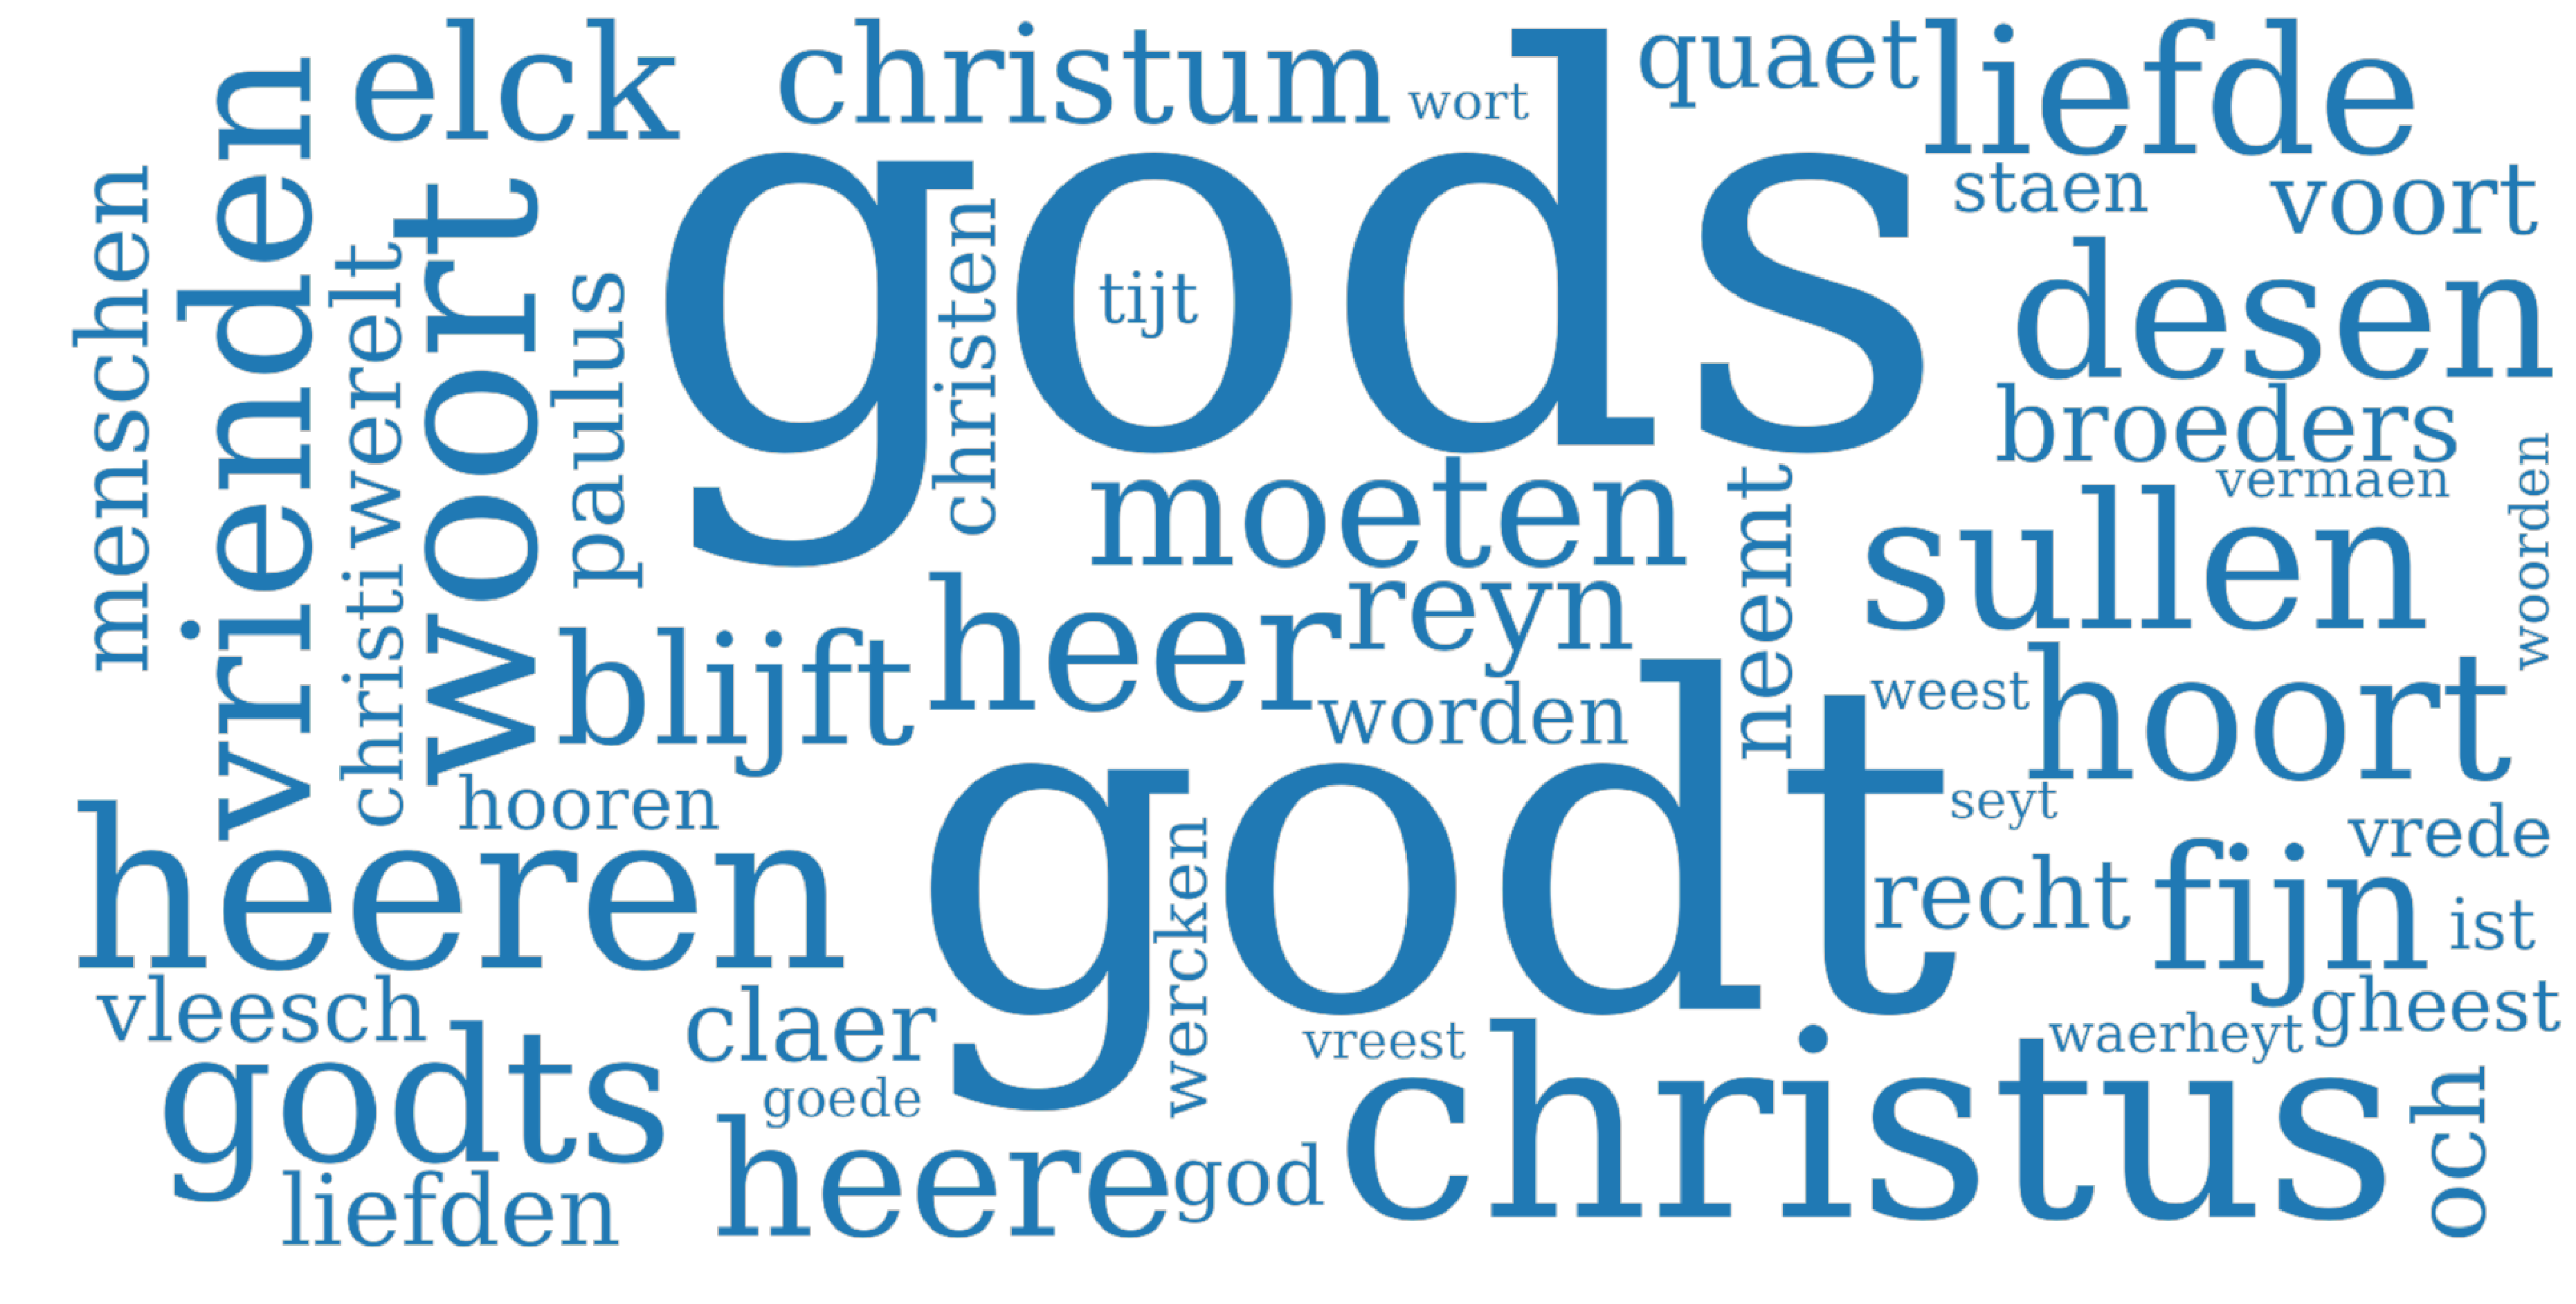
\includegraphics[width=\linewidth]{original_topic42}
		\caption{\textit{religion \& happiness} (42)}
		\label{fig:topic42Original}
		\vspace{4ex}
	\end{minipage}%%
	\begin{minipage}[c]{0.48\linewidth}
		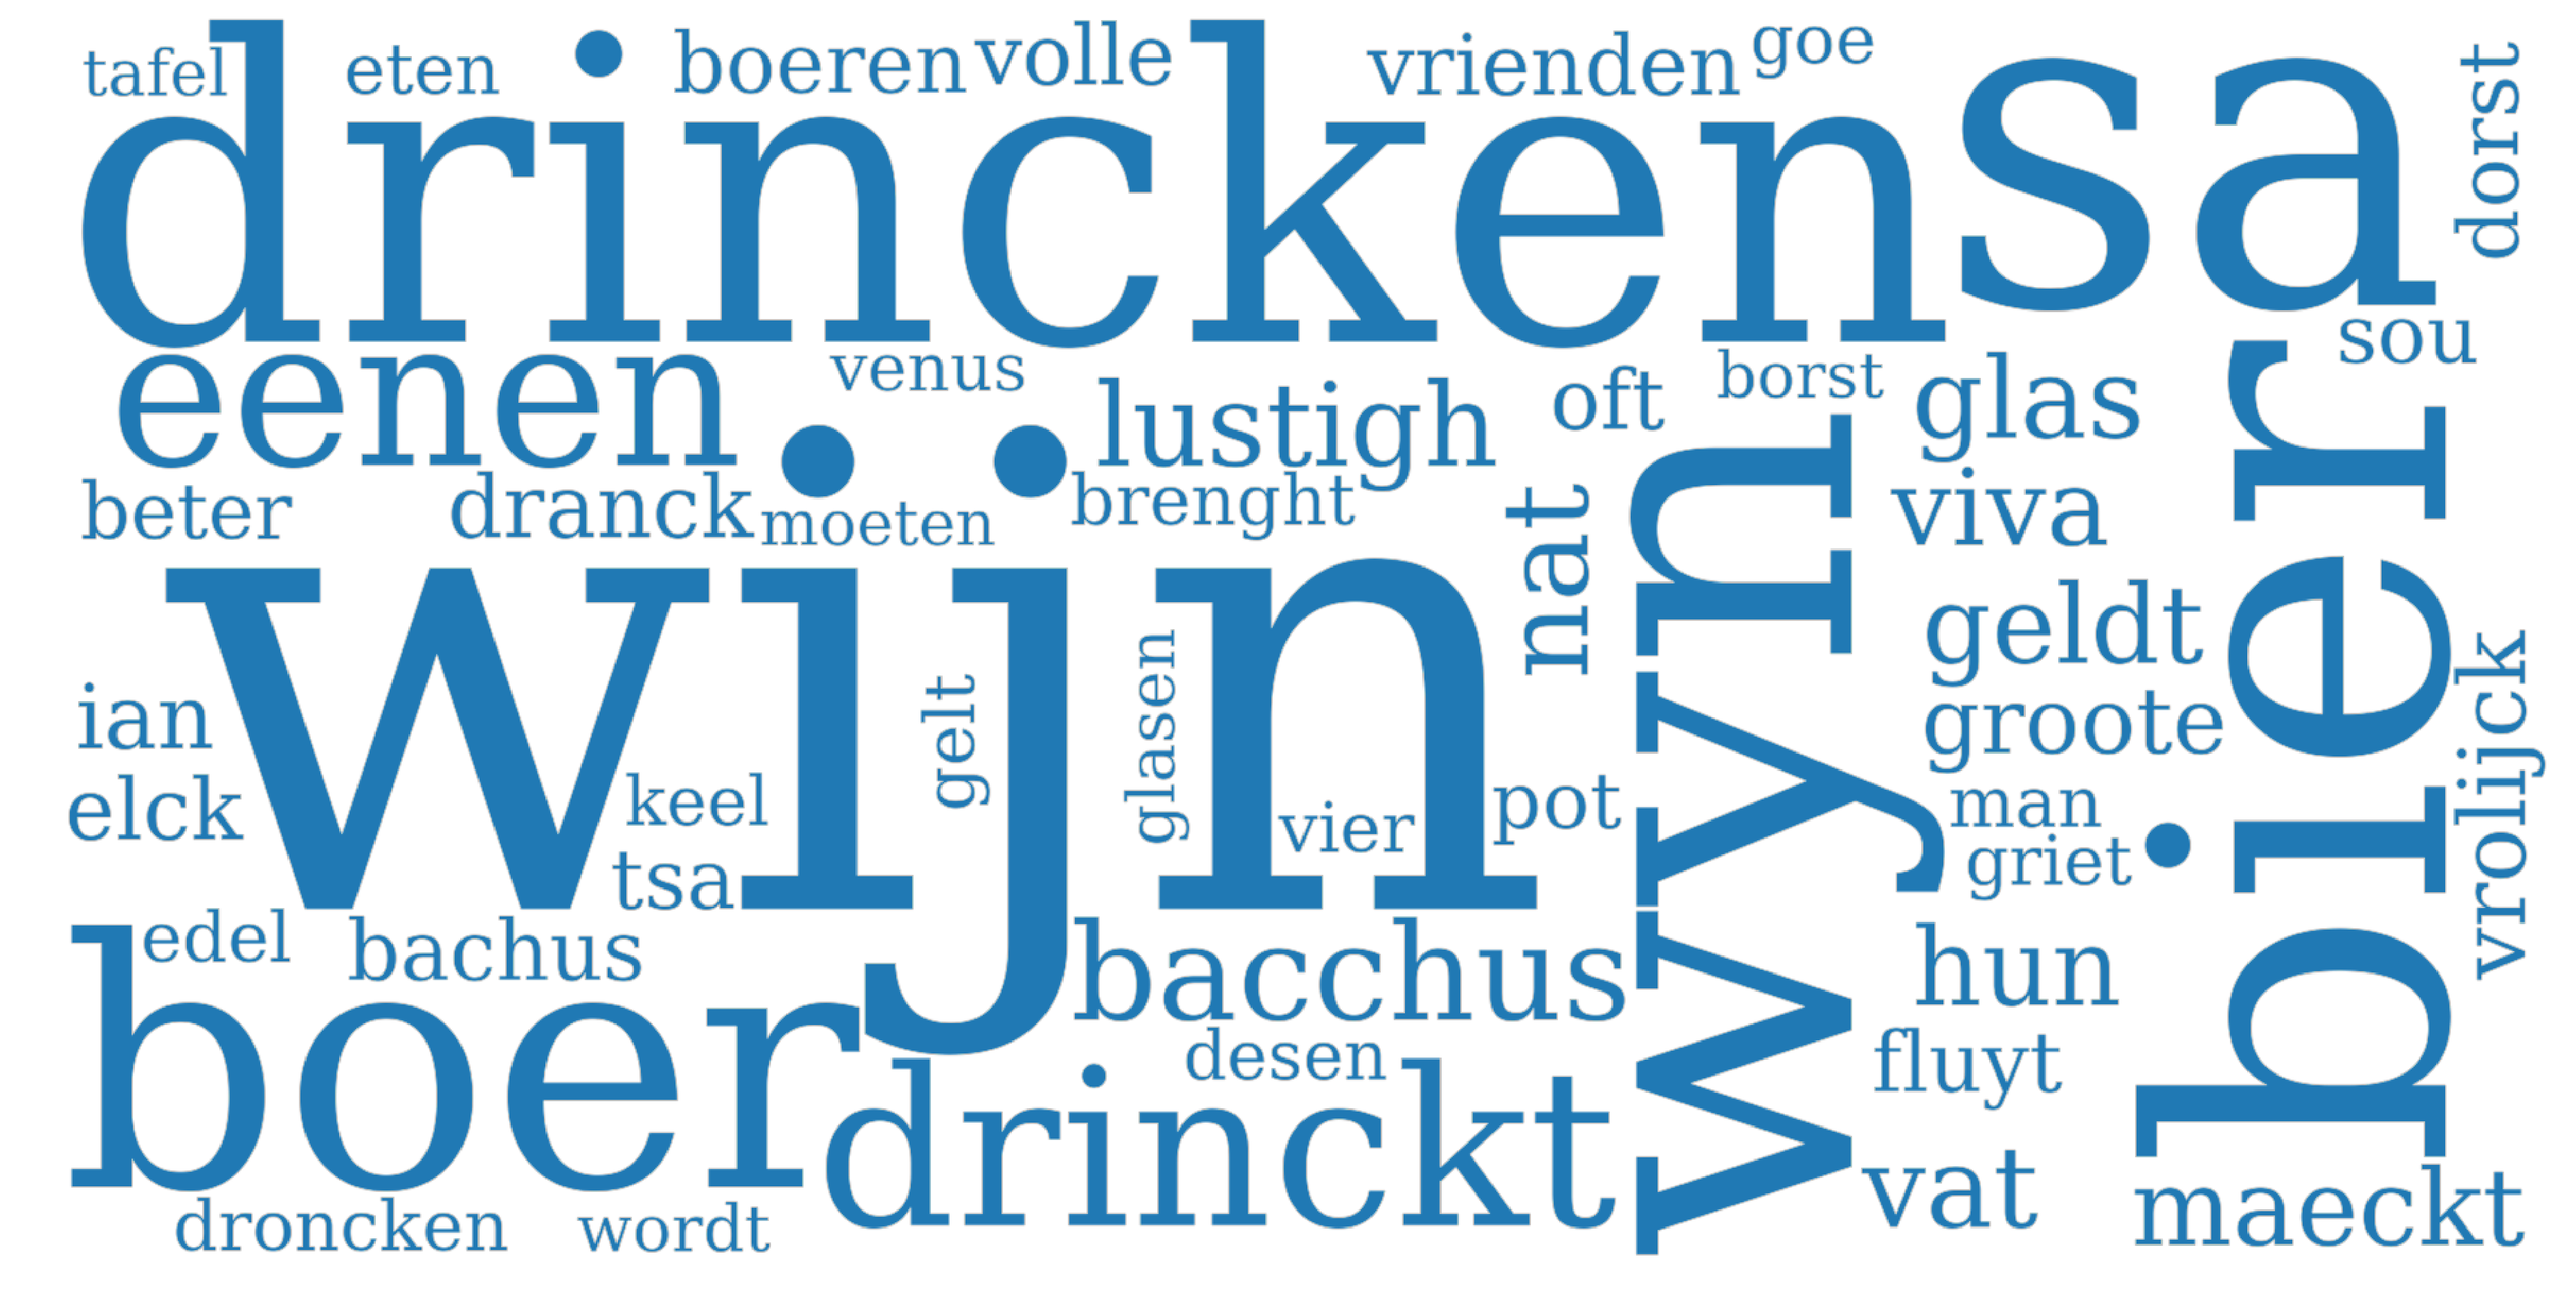
\includegraphics[width=\linewidth]{original_topic43}
		\caption{\textit{drinking} (43)}
		\label{fig:topic43Original}
		\vspace{4ex}
	\end{minipage}%%
	\hfill
	\begin{minipage}[c]{0.48\linewidth}
		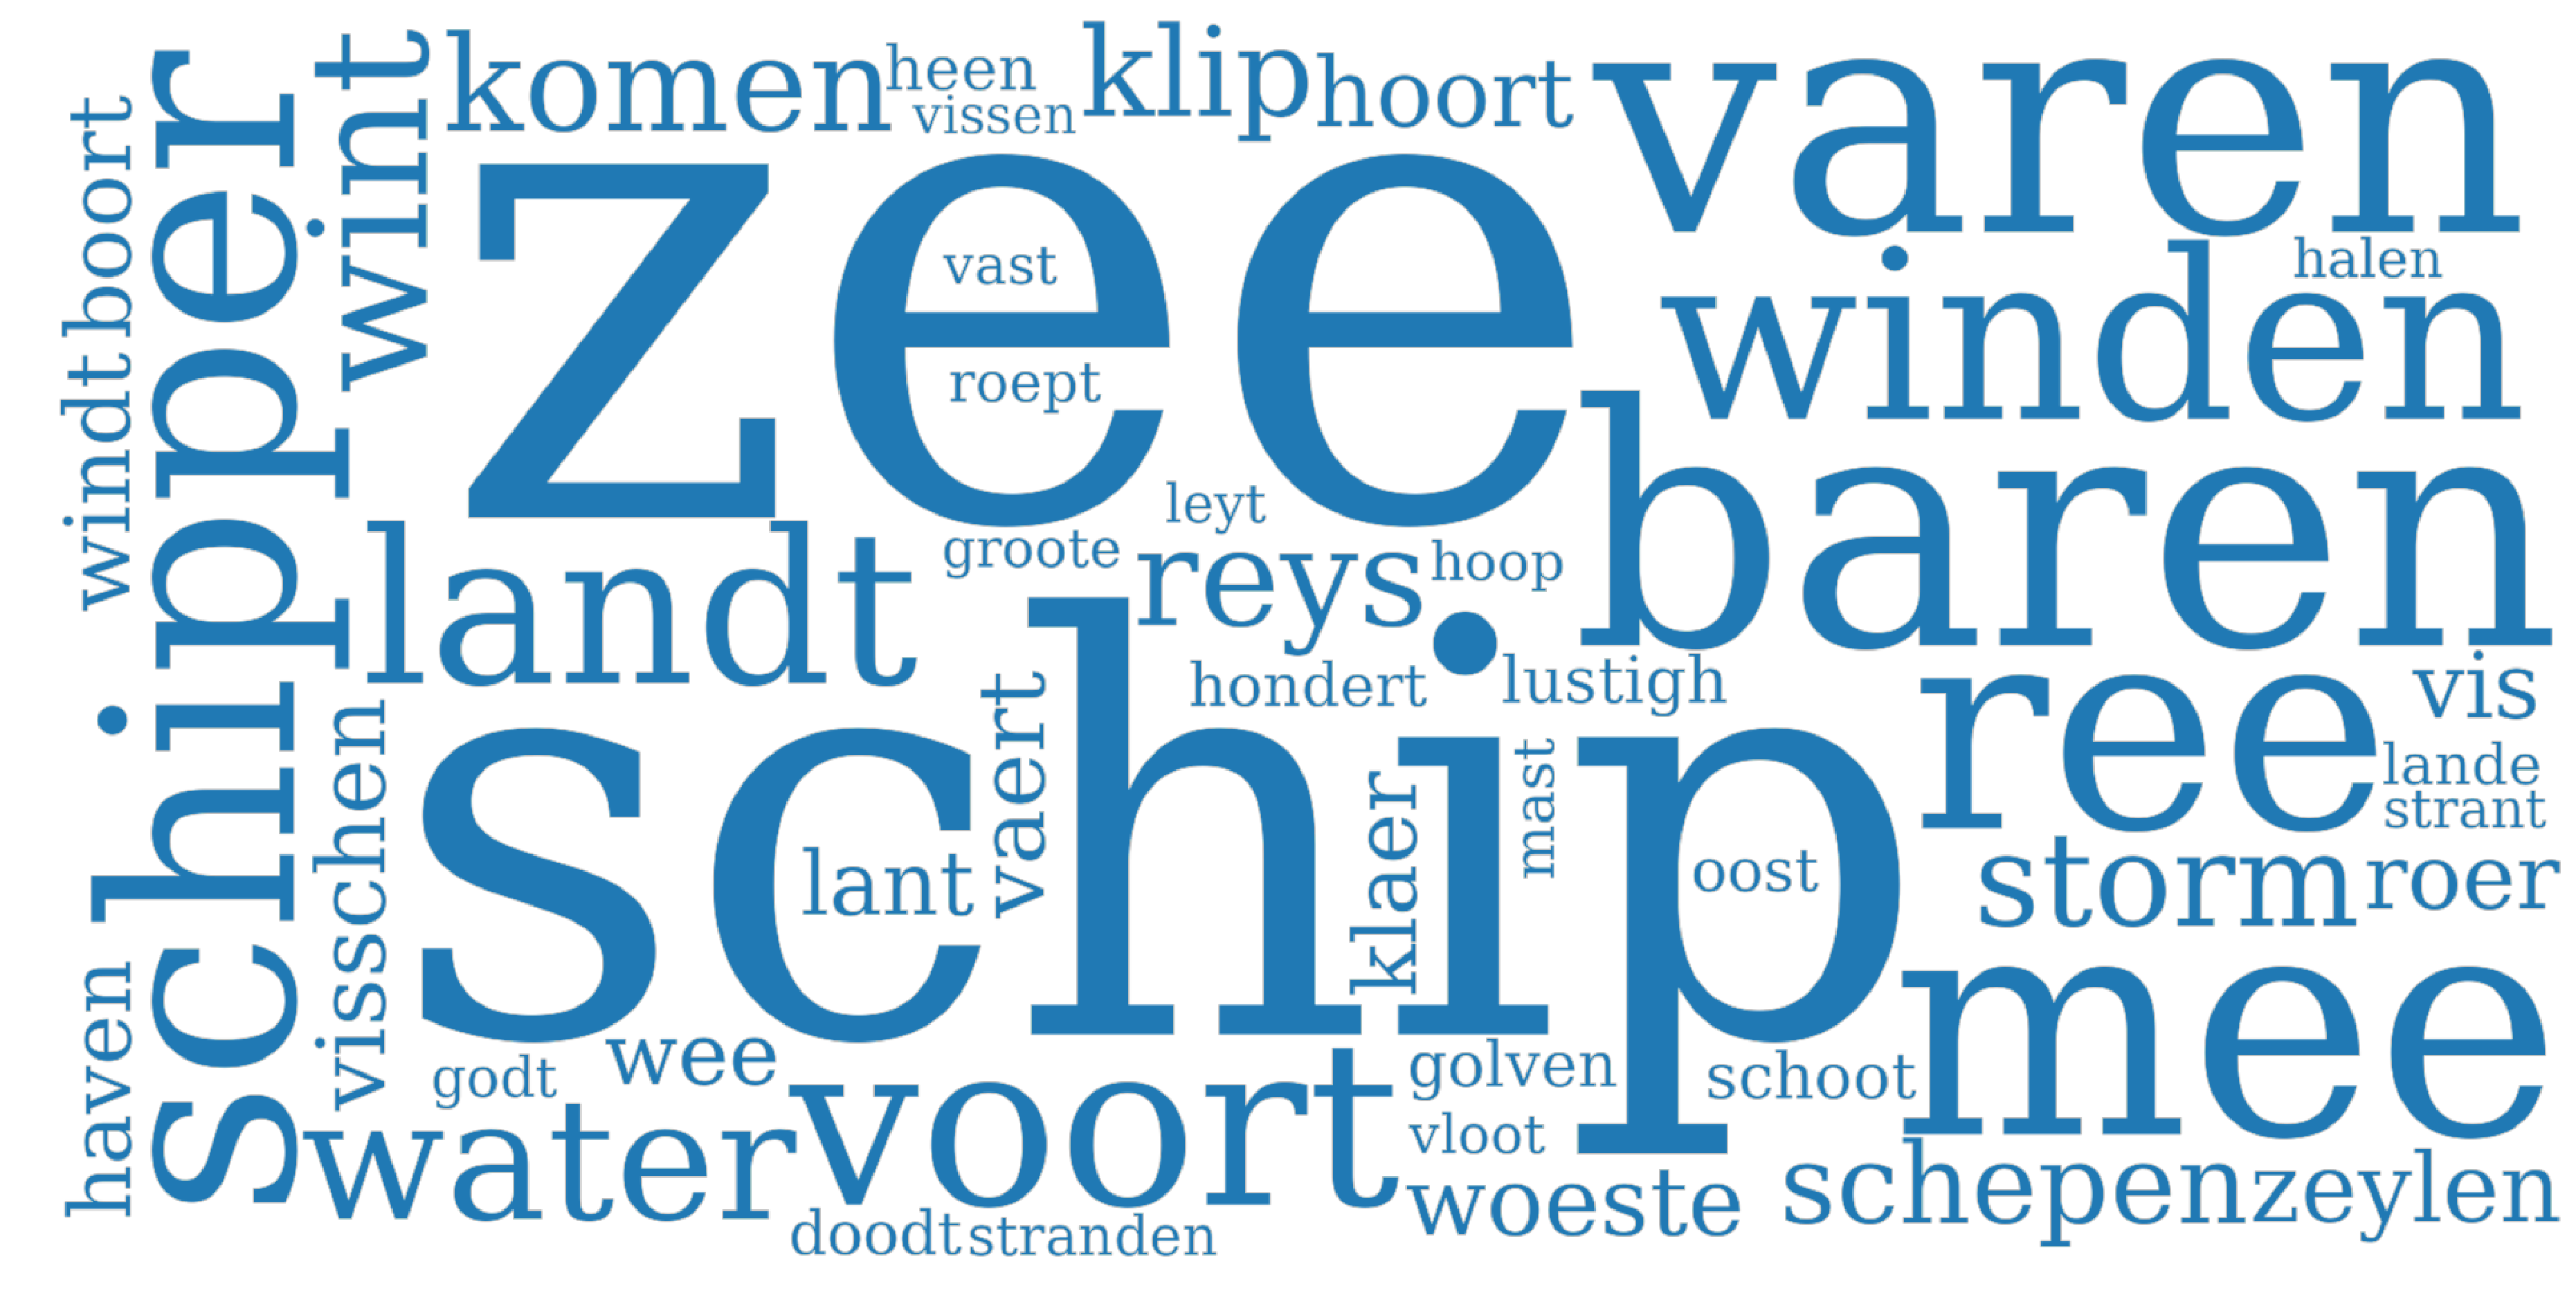
\includegraphics[width=\linewidth]{original_topic46}
		\caption{\textit{sea} (46)}
		\label{fig:topic46Original}
		\vspace{4ex}
	\end{minipage}%%
	\begin{minipage}[c]{0.48\linewidth}
		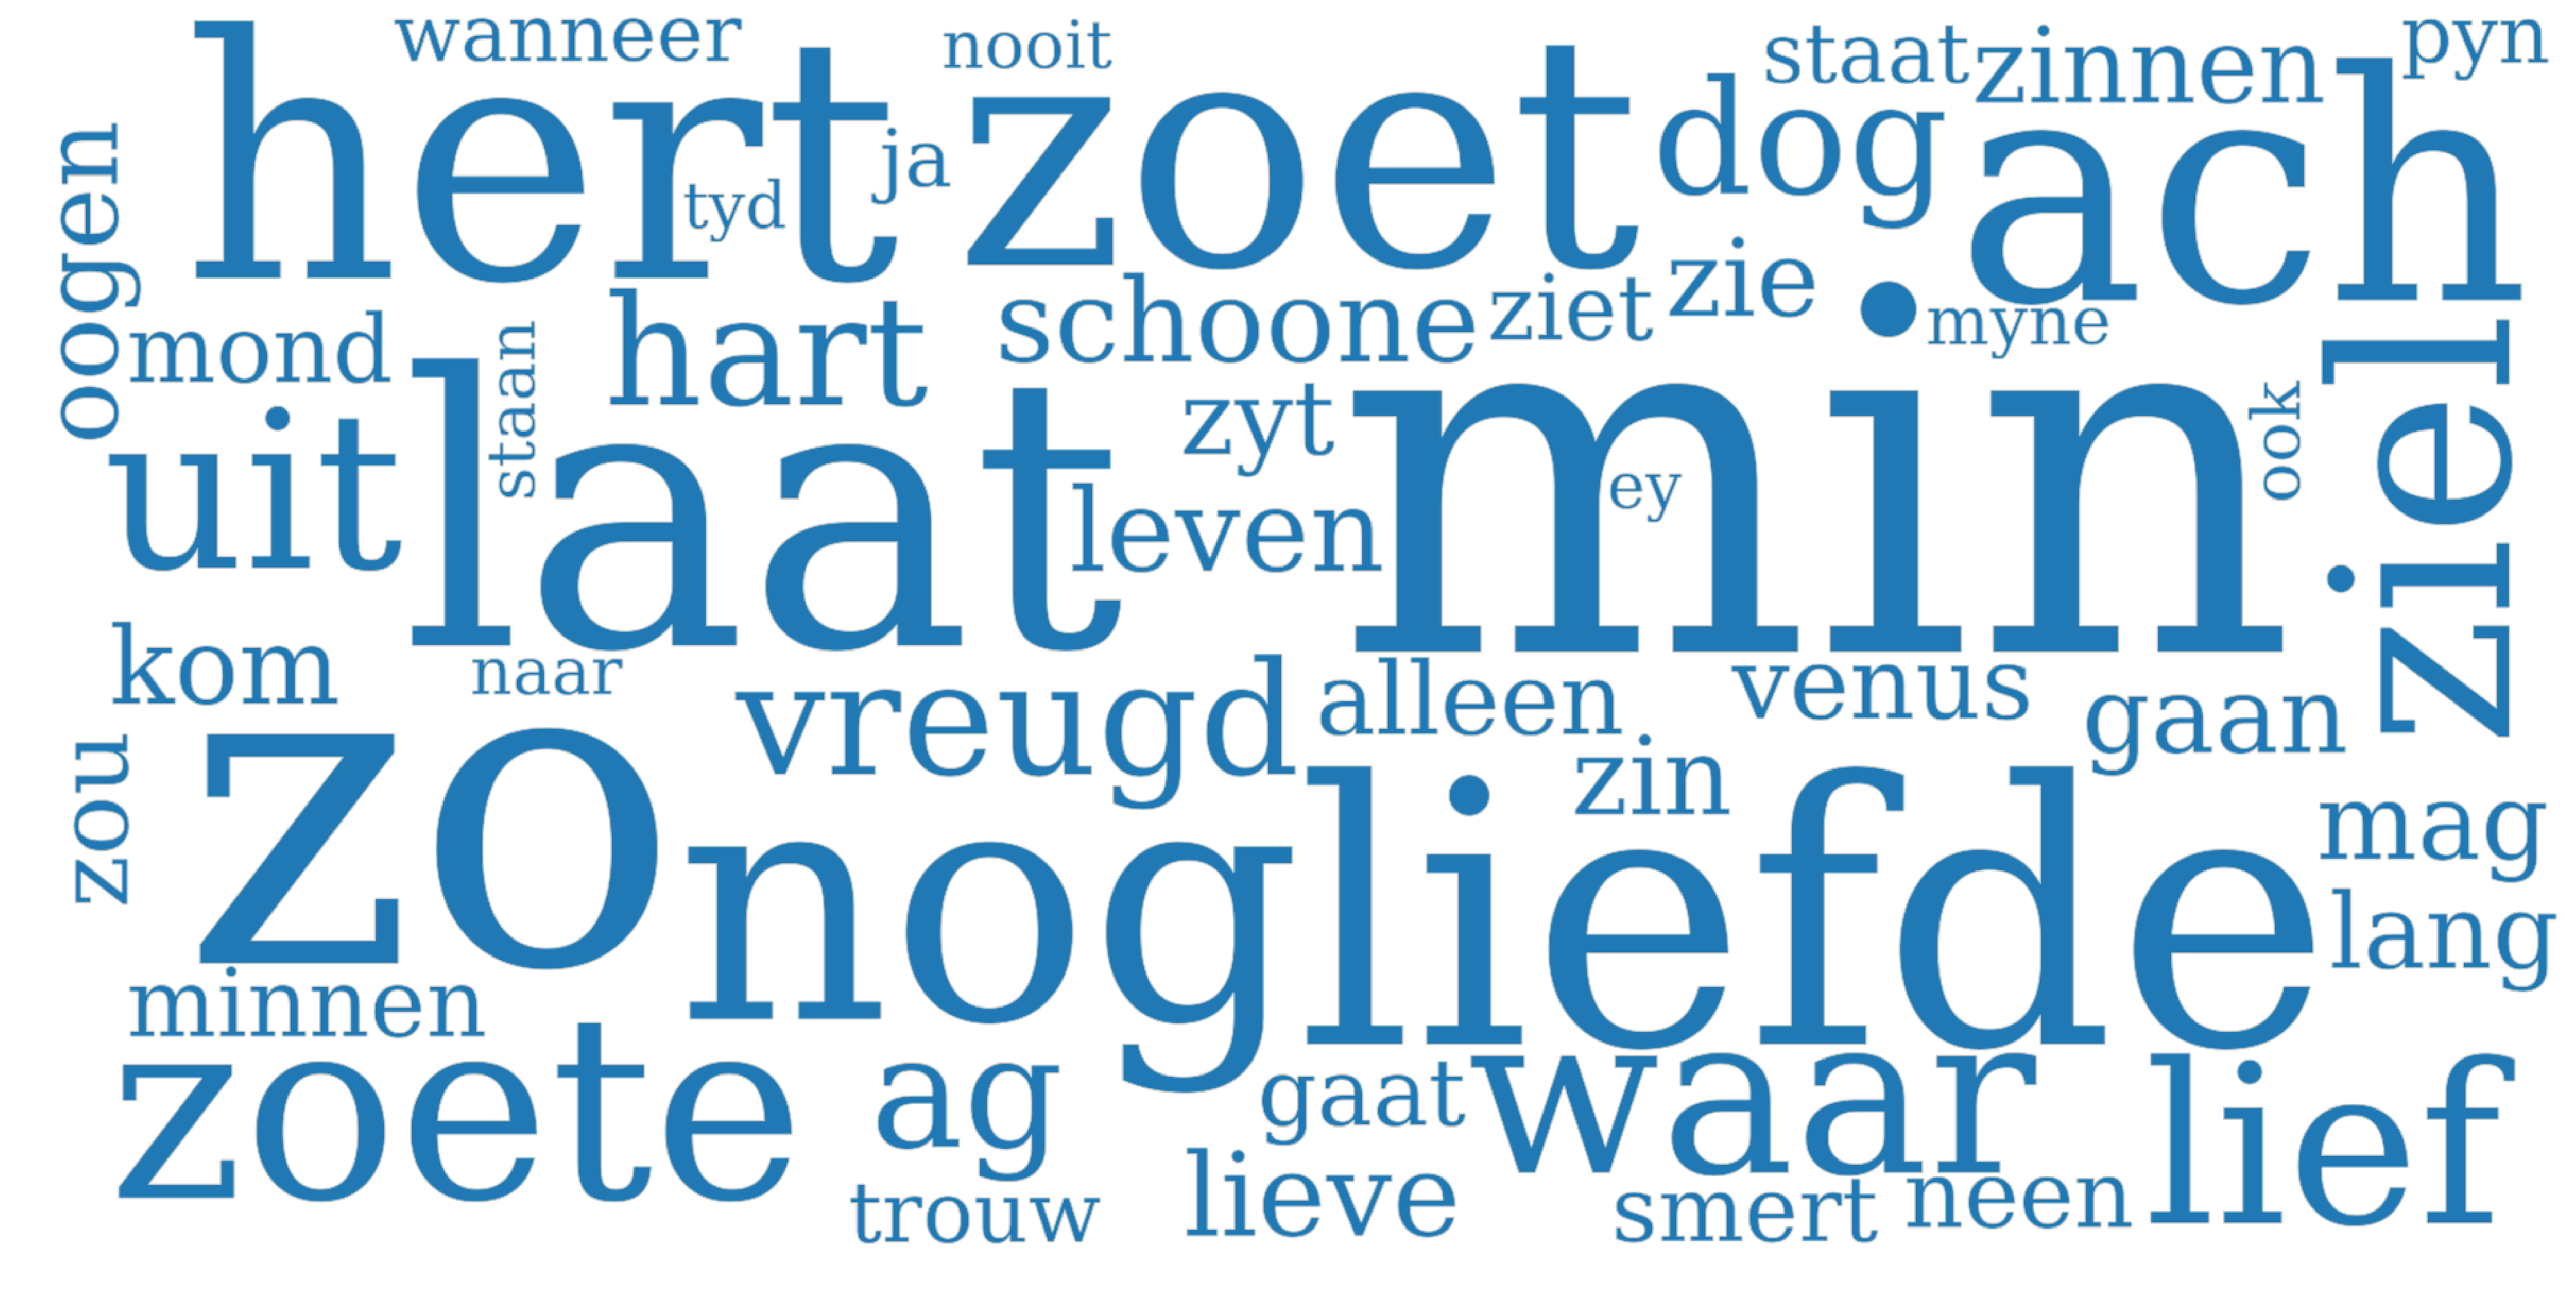
\includegraphics[width=\linewidth]{original_topic49}
		\caption{\textit{love \& happiness} (49)}
		\label{fig:topic49Original}
		\vspace{4ex}
	\end{minipage}%%
\end{figure}

Topic 7 (Figure~\ref{fig:topic7Original}) can easily be recognized as \textit{Christmas}, due to words as \enquote{kindeken}, \enquote{stal}, \enquote{maria}, \enquote{bethlehem}, \enquote{geboren} and \enquote{kindt}. To topic 10 (Figure~\ref{fig:topic10Original}), I refer with \textit{nation \& country}: the words \enquote{prins}, \enquote{soldaten}, \enquote{geusen} and \enquote{oranje} leave no doubt that these are words from political songs. In topic 12 (Figure~\ref{fig:topic12Original}), words from pastoral or bucolic poetry are clustered: many words refer to the shepherd life, such as \enquote{herder}, \enquote{vee} and \enquote{schaepjes}. Less prominent, but still present in this topic, is the name \enquote{laura} and the words \enquote{lieve} and \enquote{lief}, which suggests that not only the love for nature is chanted in these songs. I assign the subject \textit{bucolic songs} to this topic. Topic 42 (Figure~\ref{fig:topic42Original}) seems a very general religious topic with words as \enquote{gods}, \enquote{godt}, \enquote{christus} and \enquote{heeren}, all be it that almost only positive emotions are mentioned: \enquote{reyn}, \enquote{fijn}, \enquote{liefde}, \enquote{vrienden} and \enquote{vrede}. Therefore I assign the subject \textit{religion \& happiness} to this topic. Topic 43 (Figure~\ref{fig:topic43Original}) can easily be recognized as \textit{drinking}. All kinds of references to drinking are clustered in this topic, such as \enquote{drincken}, \enquote{wijn}, \enquote{bier}, \enquote{droncken} and \enquote{glas}, accompanied by words as \enquote{bacchus} (the Roman god of the wine) and \enquote{viva}. In topic 46 (Figure~\ref{fig:topic46Original}) words that refer to the life on sea are found: \enquote{zee}, \enquote{schip}, \enquote{varen}, \enquote{winden} and \enquote{baren}. I assign the word \textit{sea} to this topic. To the groups of words that are not depicted here in word clouds, I assigned a topic as well. It turns out that a lot of topics have something to do with religion. This is not surprising at all, since Table~\ref{table:SongsCat} already showed that almost 40\% of the corpus are songs from the category \enquote{religion}. In some cases it is quite easy to determine a certain subcategory (such as \textit{religion \& eternity}, \textit{religion \& happiness}, \textit{ religion \& sin}), but for a lot of religious topics the difference is not easy to distinguish.

However, I do not know yet which topics are more dominant in the corpus than the others. Each song receives a distribution over all the topics. This means that, for each song,  the sum of contributions of topics is always 1. Ideally, there is for each song one topic which is way more dominant than the 49 others. To see which topics are the most dominant in my corpus, I choose for each song the topic that has the highest contribution, using the following code:

\begin{lstlisting}
	transformed_docs = lda.load_document_topics()
	docs = [[texts[i]] + [r[0] for r in list(zip(max(row, key=lambda x:x[1])))] for i, row in enumerate(transformed_docs)]
	dominant_topics = pd.DataFrame(docs, columns=["document_id", "dominant_topic", "perc_contribution"])
\end{lstlisting}

\begin{table}
	\begin{minipage}{0.5\textwidth}
		\begin{tabular}{ccl}
			\toprule
			Topic & Songs & Subject \\
			\midrule
			49             &  1377 & love \& happiness \\
			3              &  1078 & love \& sadness \\
			21             &   993 & religion \& eternity \\
			0              &   993 & religion \\
			40             &   962 & religion \& emotions \\
			24             &   787 & religion \\
			42             &   770 & religion \& happiness \\
			13             &   753 & rejection \\
			30             &   704 & religion \\
			18             &   703 & ??? \\
			26             &   698 & virtuous life \\
			32             &   695 & physical love \\
			25             &   646 & religion \\
			4              &   643 & religion \& praise \\
			39             &   637 & verbs \\
			29             &   579 & love \& consolation \\
			9              &   511 & religion \\
			23             &   483 & religion \& sin \\
			15             &   429 & religion \& virtues \\
			28             &   413 & religion \\
			27             &   403 & death \& passion\\
			7              &   389 & Christmas \\
			12             &   381 & bucolic songs \\
			44             &   365 & religion \\
			22             &   351 & religion \\
			\vdots & \vdots & \vdots \\
			\bottomrule
		\end{tabular}
	\end{minipage} \hfill
	\begin{minipage}{0.5\textwidth}
		\begin{tabular}{|ccl}
			\toprule
			Topic & Songs & Subject \\
			\midrule
			\vdots & \vdots &\vdots \\
			
			43             &   350 & drinking \\
			19             &   338 & religion \\
			1              &   337 & religion \& Mary \\
			41             &   328 & love \& happiness \\
			8              &   315 & love \\
			48             &   305 & profane love \\
			31             &   265 & marriage \\
			14             &   262 & verbs \\
			10             &   250 & nation \& country \\
			36             &   248 & verbs \\
			38             &   246 & nature \\
			35             &   244 & religion \\
			11             &   241 & religion \\
			20             &   238 & German/French \\
			33             &   219 & God \& nation \\
			2              &   197 & God \& church \\
			47             &   178 & old spelling \\
			6              &   163 & ??? \\
			46             &   144 & sea \\
			16             &   133 & pronouns \\
			37             &   125 & Old Testament \\
			17             &   116 & love \& Jesus \\
			45             &   113 & ??? \\
			34             &   110 & trash \\
			5              &    89 & verbs \\
			\bottomrule
		\end{tabular}
	\end{minipage}
	\caption{Dominant topics in original corpus (\textit{n} = 22,297)}
	\label{table:DomTopOr}
\end{table}

\noindent Subsequently, I group the dominant topics and count how many times they appear in the dataframe \texttt{dominant\_topics}:

\begin{lstlisting}
topic_counts = dominant_topics["dominant_topic"].value_counts()
topic_contribution = round(topic_counts/topic_counts.sum(), 4)
df_dominant_topics = pd.concat([topic_counts, topic_contribution], axis=1)
df_dominant_topics.columns = ["Num_Documents", "Perc_Documents"]
\end{lstlisting}

\noindent The results are stored in Table~\ref{table:DomTopOr}. It is important to realize that the sum of songs in this table is 22,297, which means that, for now, only the \enquote{original} songs are included, and not their reprints and appearances in other songbooks. That is a step I will take in a later stadium, after I have evaluated the three different models.

A tool that can help to get more insight in the topics and how they are related to each other, is the Python package \texttt{pyLDAvis}, which is a library for interactive topic model visualization. The package extracts information from a fitted LDA topic model to inform an interactive web-based visualization. In order to visualize my topic model, made with the MALLET wrapper of \texttt{gensim}, I first have to convert it to a \enquote{normal} LDA model in \texttt{gensim}. Afterwards, I import the converted model into the \texttt{pyLDAvis prepare}-function:

\begin{lstlisting}
model = gensim.models.wrappers.ldamallet.malletmodel2ldamodel(lda)

import pyLDAvis
import pyLDAvis.gensim

pyLDAvis.enable_notebook()
vis = pyLDAvis.gensim.prepare(model, corpus, dictionary, sort_topics=False)
\end{lstlisting}

\noindent With \texttt{sort\_topics=False}, I make sure that the same topics are used as the ones in the original model, made with \texttt{gensim.models.wrappers.LdaMallet}. The output is a so-called Intertopic Distance Map, with multidimensional scaling. The screenshot in Figure~\ref{fig:pyLDAvisOriginal} gives an impression how the interactive visualization looks like. Each bubble on the left-hand side plot represents a topic. The larger the bubble, the more prevalent the topic is. An important note is that \texttt{pyLDAvis} starts counting at 1, while the topics made with \texttt{gensim} start at 0. Each number $x$ in the \texttt{pyLDAvis}-plot therefore corresponds with topic $x-1$. If you hover over the different topics at left, at right the most relevant terms for the topic in question are displayed.

\begin{figure}[hbt!]
	\centering
	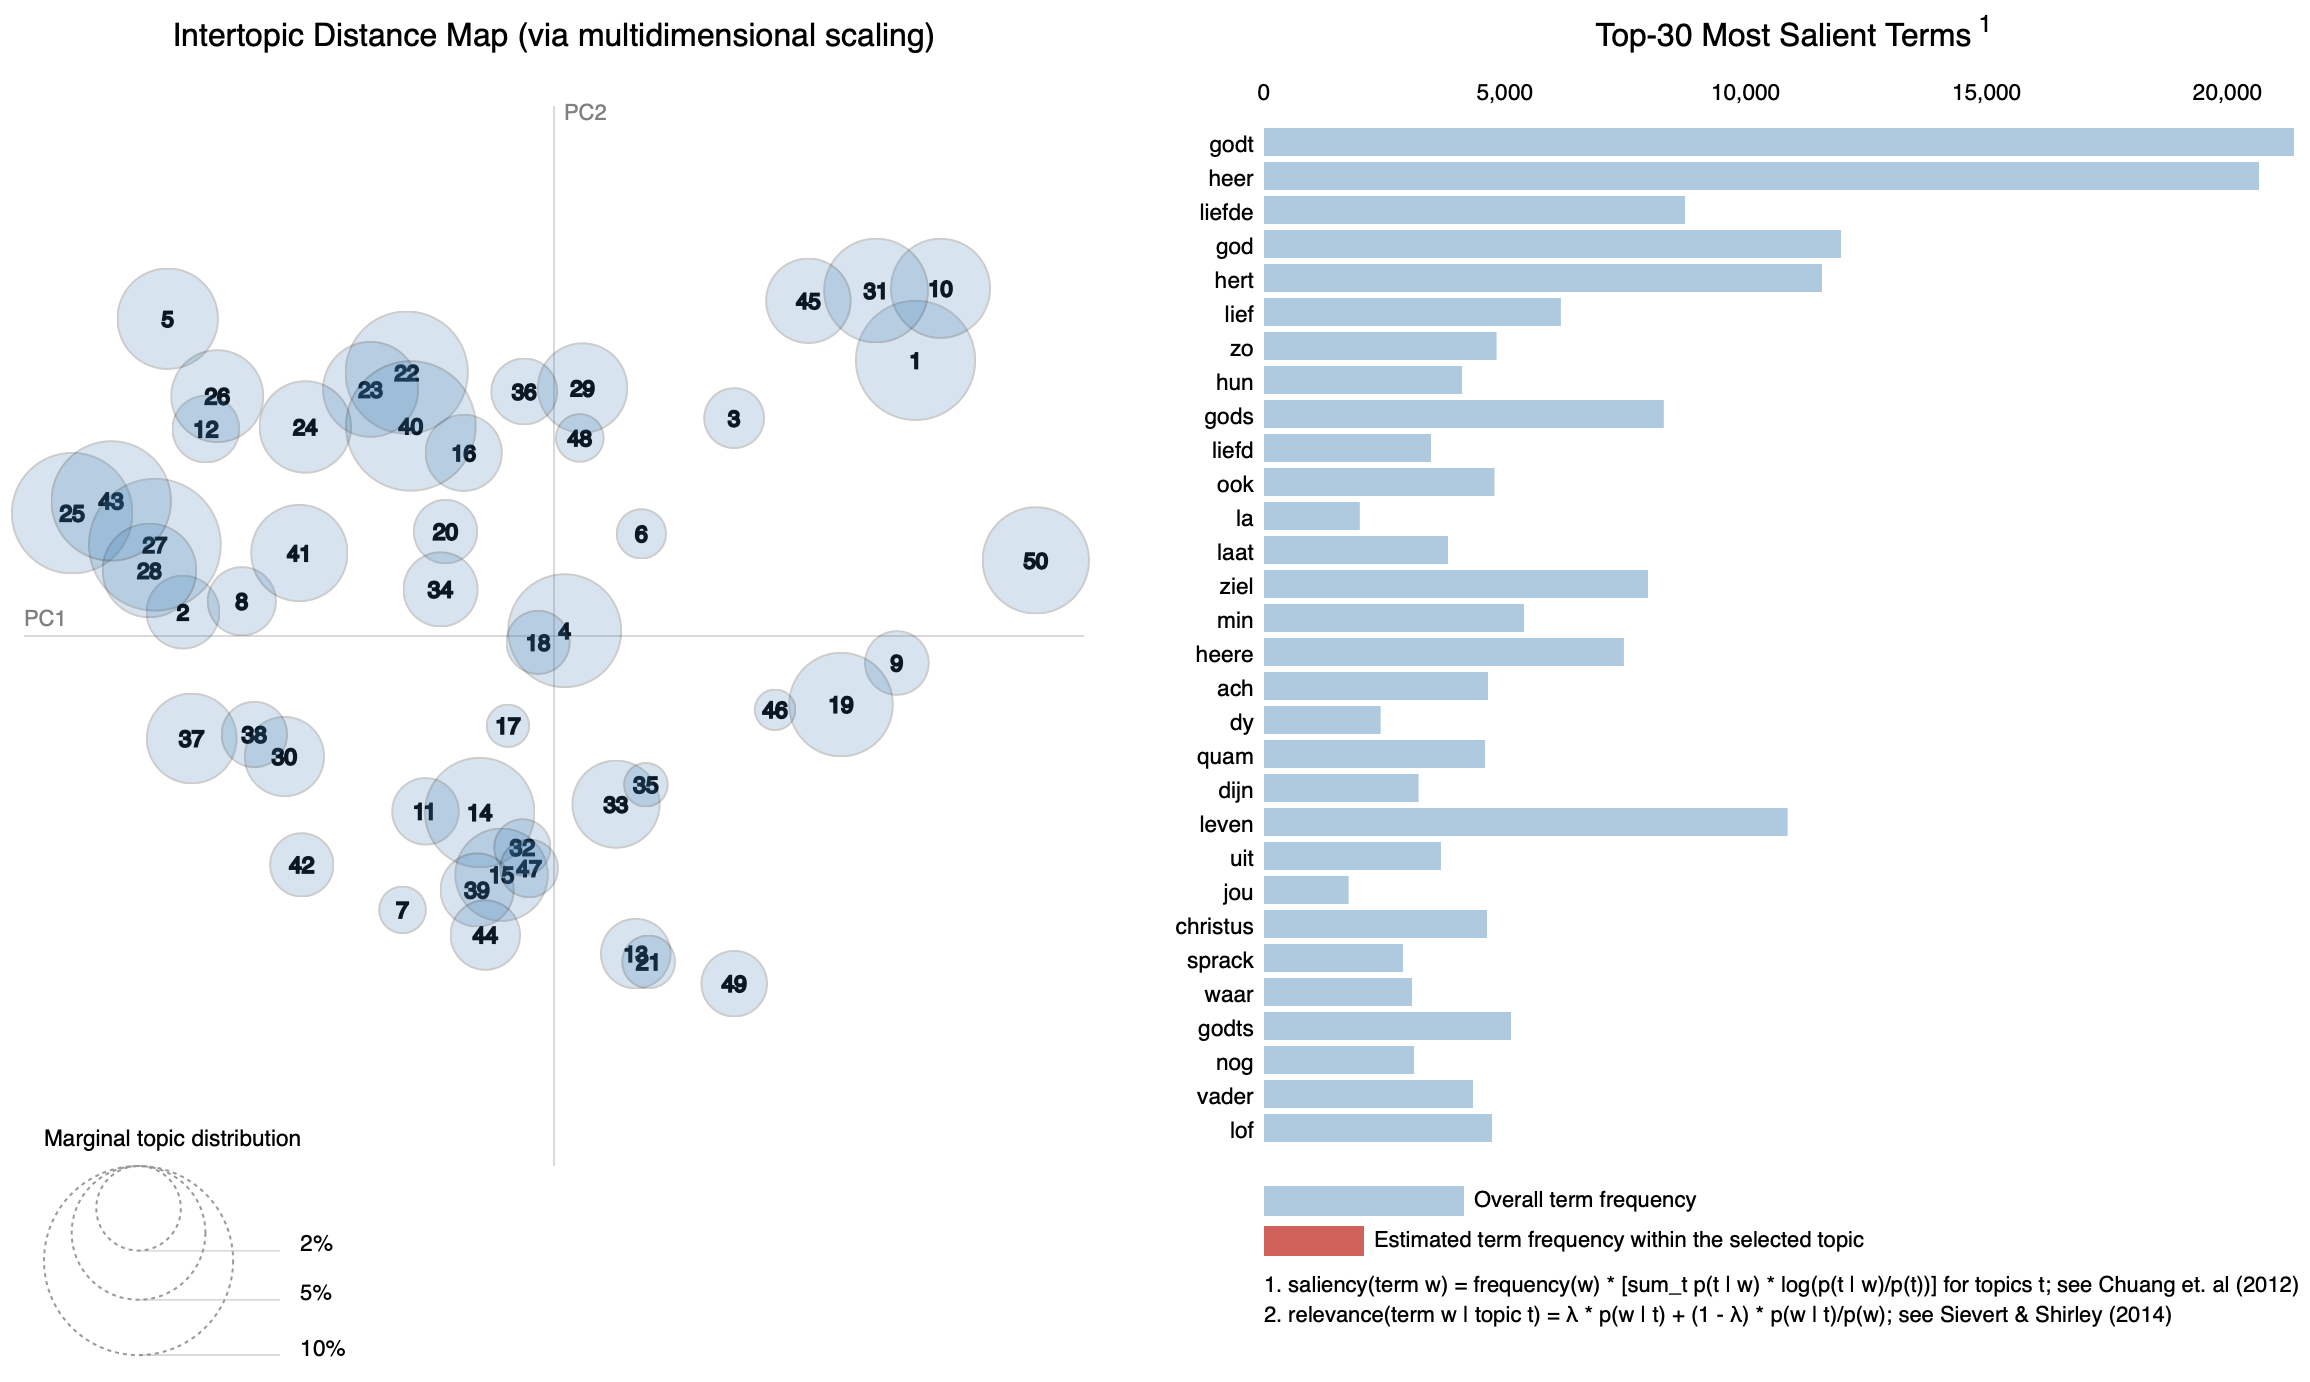
\includegraphics[scale=0.3]{original_pyLDAvis}
	\caption{Visualization of topics in the original corpus with \texttt{pyLDAvis}}
	\label{fig:pyLDAvisOriginal}
\end{figure}

\noindent A good topic model should have bubbles scattered throughout the chart, instead of being clustered in one quadrant. A model with too many topics will typically have many overlapping small sized bubbles clustered in one region of the chart. Although the bubbles in Figure~\ref{fig:pyLDAvisOriginal} are scattered throughout the chart, there are quite a few small sized bubbles, and many of them are overlapping with others. When taking a closer look to the groups with topics, it turns out that the bubbles that cluster together, were also interpreted by me as comparable topics. All bubbles in the top left quadrant are religious topics, as well as some topics in the top right quadrant. When hovering over the most salient terms that are pictured in the right-hand side plot, the topics in which the word in question is represented, are shown. Figure Figure~\ref{fig:pyLDAvisOriginal_godt} confirms the notion that religious topics are clustered in the top left quadrant. The bottom left and right quadrant are filled with the more \enquote{profane} topics, with the two biggest topics on love (49 and 3 or, in Figure~\ref{fig:pyLDAvisOriginal}, 50 and 4) close to the x-axis, as a sort of divider between the two areas. Figure~\ref{fig:pyLDAvisOriginal_liefde} indeed shows that topics on love are scattered throughout the chart, but mainly represented along the x-axis.

\begin{figure}[hbt!]
	\centering
	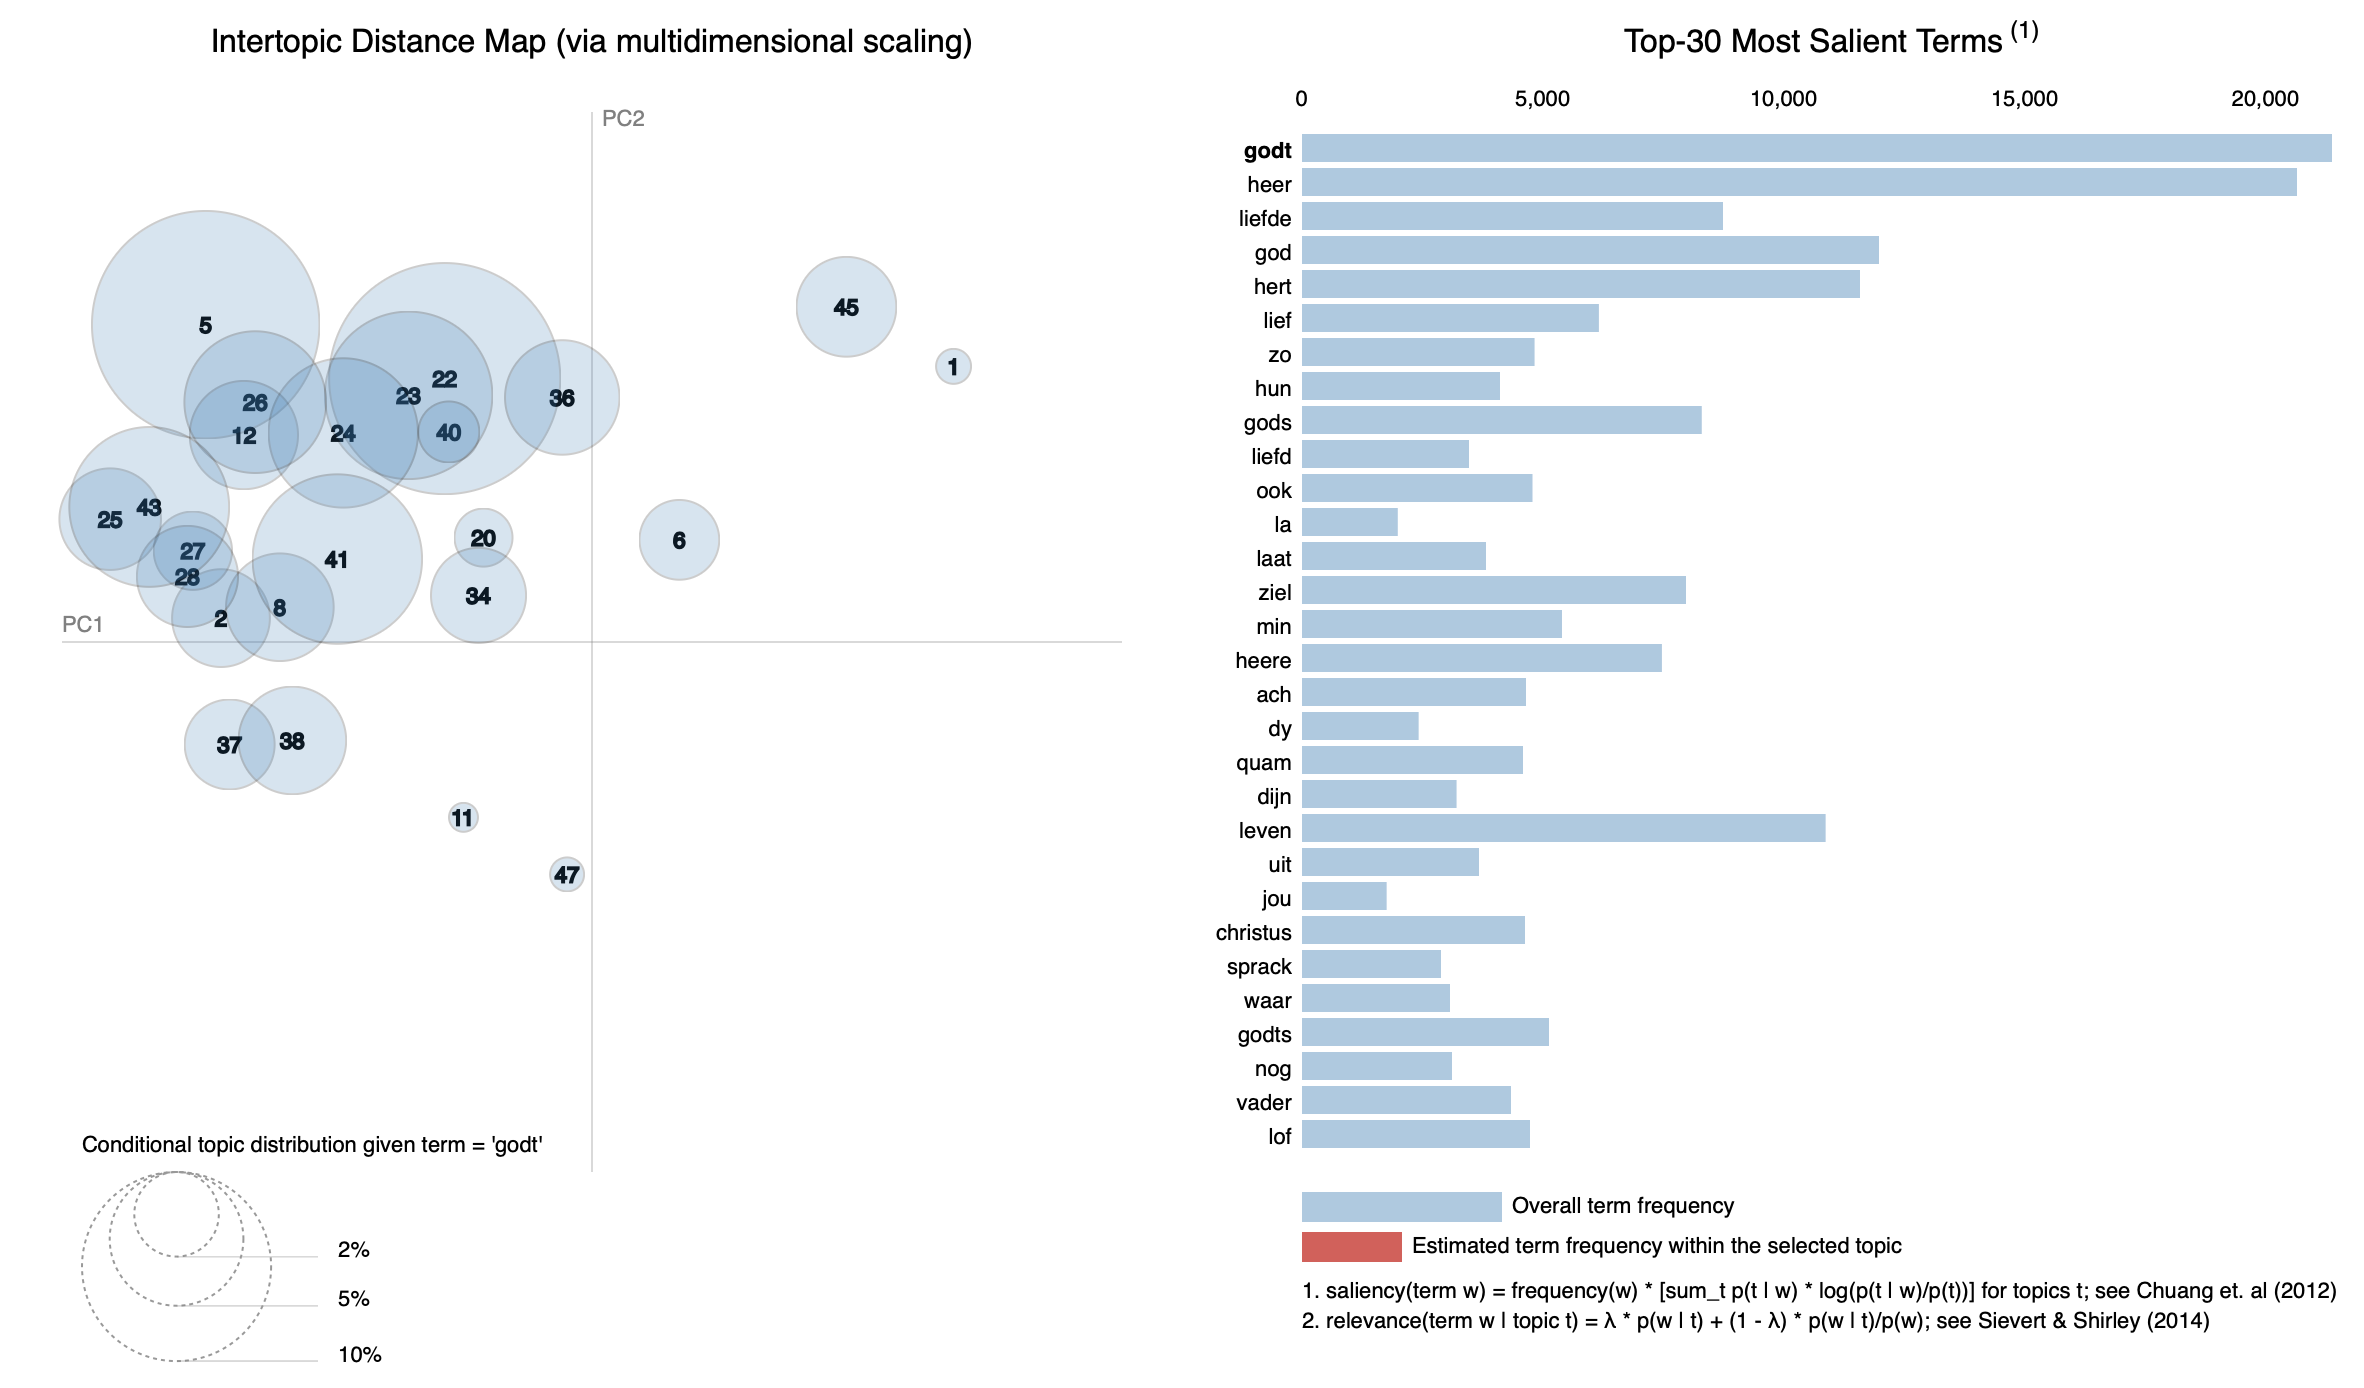
\includegraphics[scale=0.3]{original_pyldavis_godt}
	\caption{Visualization of topics with \textit{godt} in the original corpus}
	\label{fig:pyLDAvisOriginal_godt}
\end{figure}

\begin{figure}[hbt!]
	\centering
	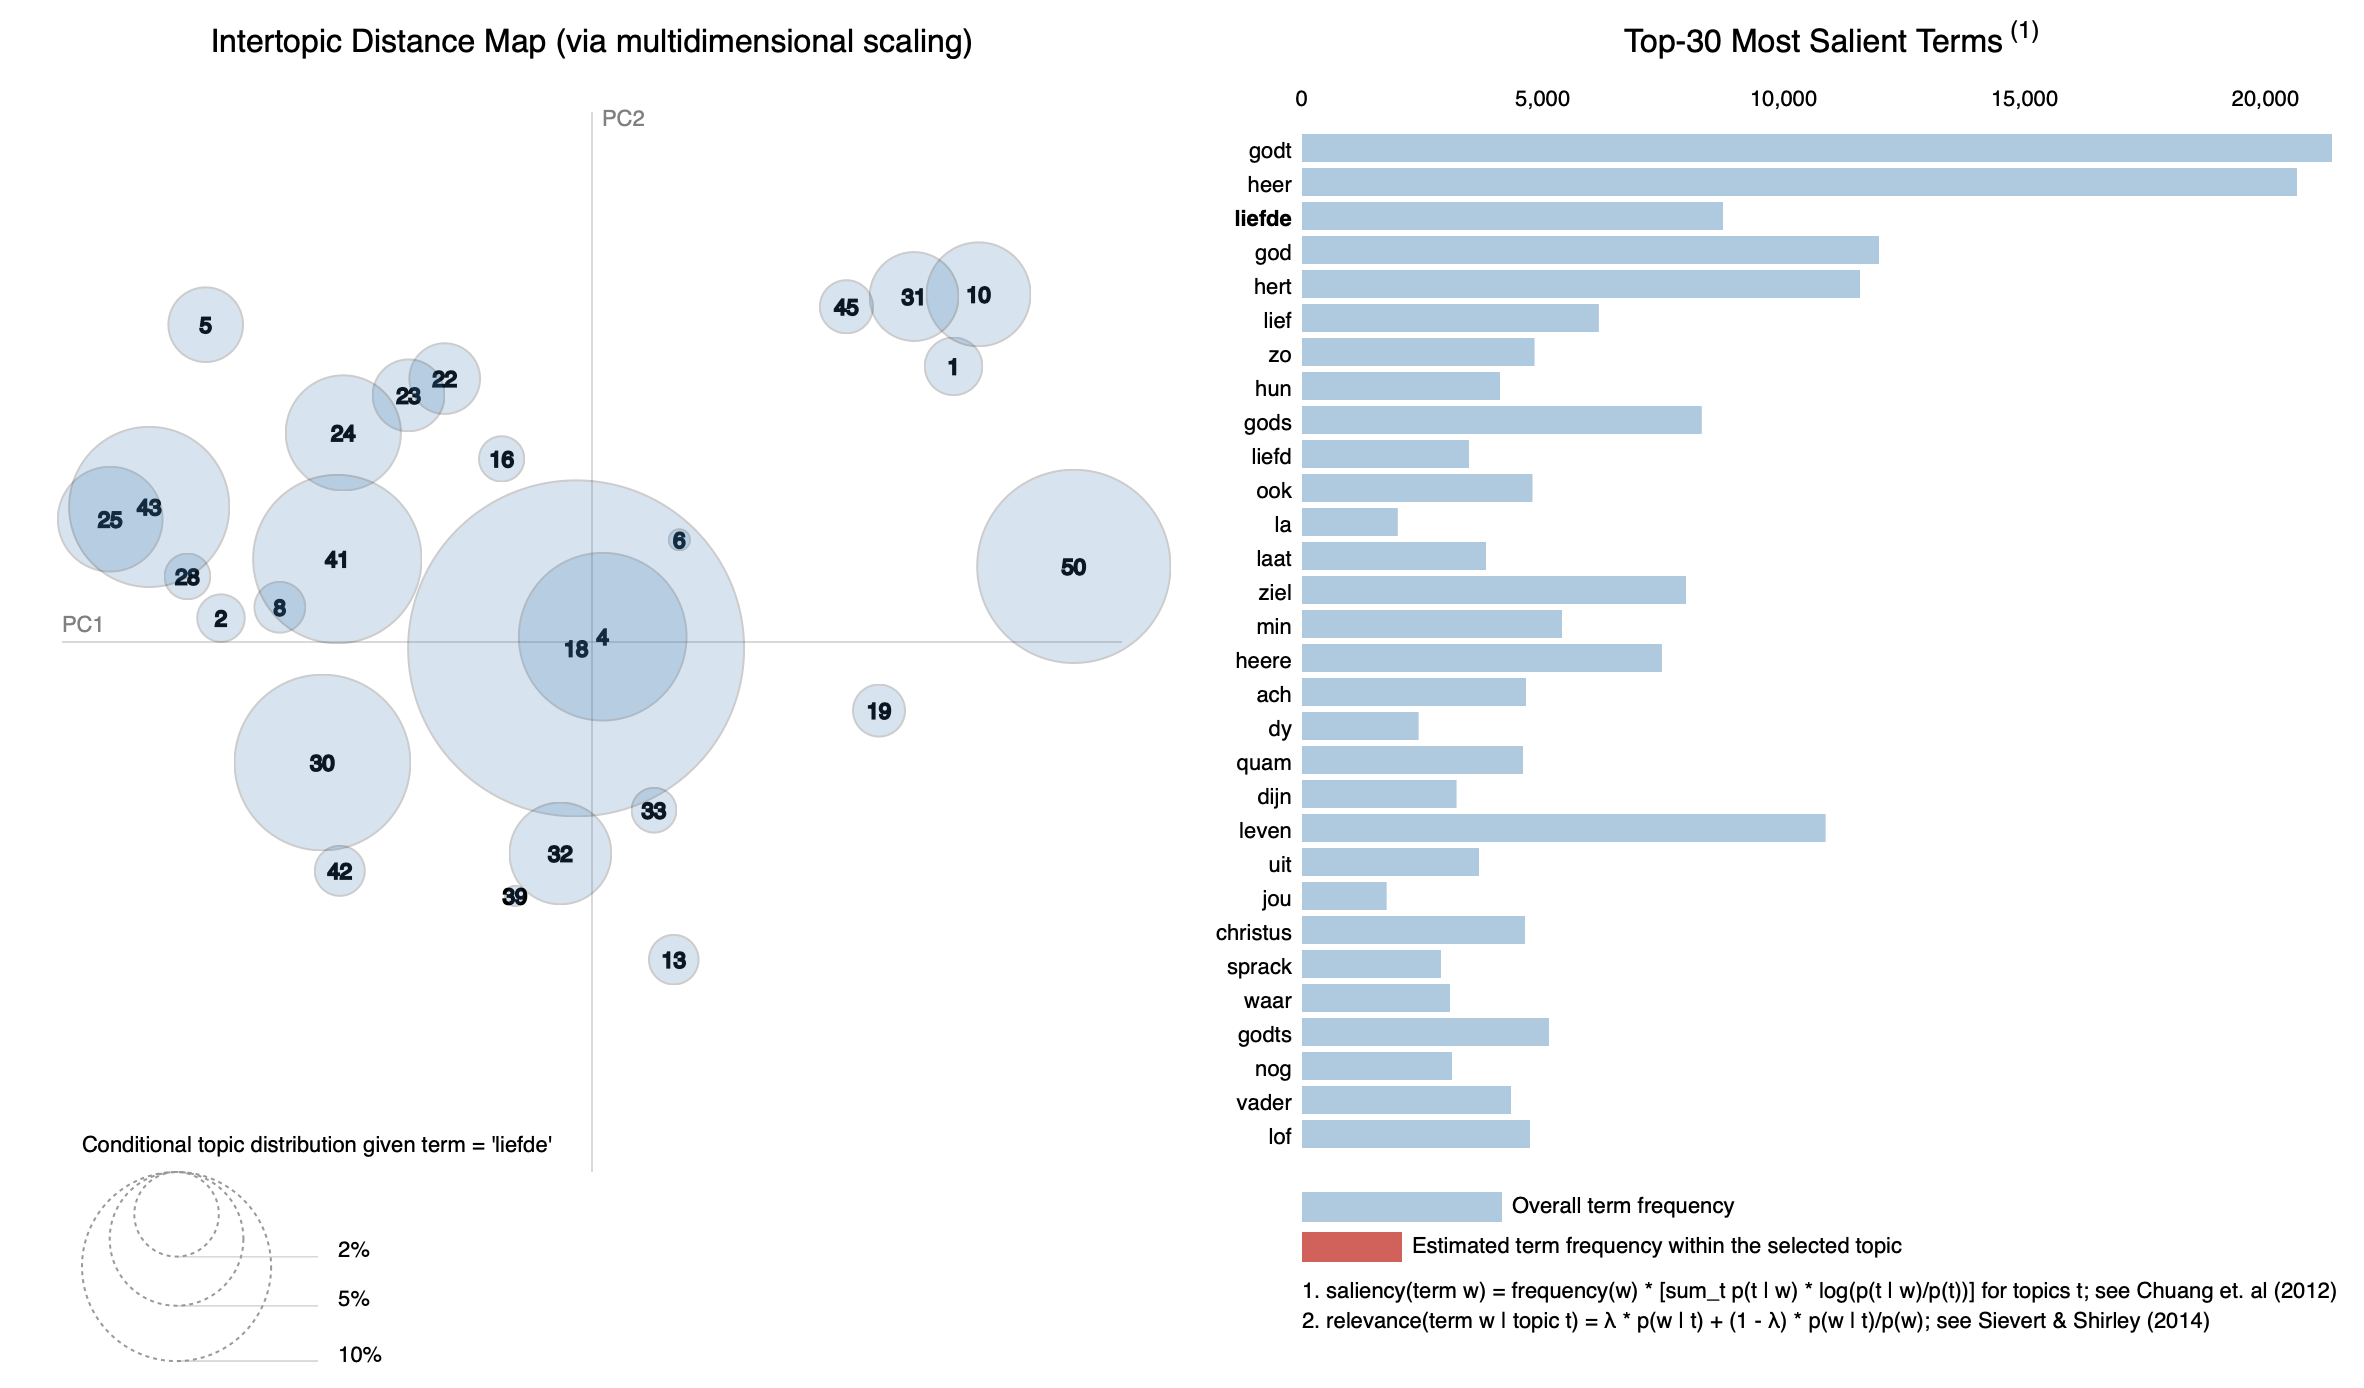
\includegraphics[scale=0.3]{original_pyldavis_liefde}
	\caption{Visualization of topics with \textit{liefde} in the original corpus}
	\label{fig:pyLDAvisOriginal_liefde}
\end{figure}

Since these topics are made from a corpus with unnormalized spelling, there are also topics in which words from a certain time period are clustered, or topics with words that make no sense at all. I shall explain this with a few examples. Topic 47 contains words spelled in a way which was very common in the fifteenth and sixteenth century, such as \enquote{ghoed}, \enquote{dyn}, \enquote{dyne}, \enquote{dyns} and \enquote{dueghd}. To topic 34 I referred as \textit{trash} in Table~\ref{table:DomTopOr}. The words \enquote{dy}, \enquote{yn}, \enquote{soe}, \enquote{uwz} and \enquote{jon} seem to be the result of either a mistake in digitization or tokenization, or a wrong printed lyric. Topic 20 makes clear that there are some songs in the corpus that are written in German or French: there is no other explanation for words such as \enquote{ich}, \enquote{das}, \enquote{je} and \enquote{vous} clustered together. Normalization of the spelling would not solve the problem of foreign songs, but it can reduce the number of topics that are built based on the time-specific spelling of the words that are in it. In the next paragraph I therefore built a topic model from the INL-normalized corpus, to see if this model outstands the one built and discussed in the current paragraph.

\subsection{INL-normalized corpus}
The dictionary that was build from the INL-normalized corpus, contained at first 186,692 unique tokens. The setting \texttt{no\_below = 2} resulted in the elimination of 114,100 tokens (the words with a value of \texttt{1} in the dictionary). The number of remaining tokens was 72,592. That is already 17,000 less words than in the dictionary of the original corpus. Again, I build a model with 50 topics. The coherence score of this model is 0.4683, which is lower than the coherence score from the previous built model. Again, I tried to assign a subject to each topic. Besides that, I investigated also which topic is the dominant for each song, and grouped the dominant topics to count how many times they appear. The results of both actions are stored in Table~\ref{table:DomTopINL}.

While assigning subjects to the topics that were composed from the INL-normalized corpus, I noticed that this time, when compared to the topics composed from the original corpus, much more topics were inconclusive and therefore hard to assign a subject to. Topic 38 and topic 15 for example are in the Top10 most dominant topics, but their subject is almost impossible to distill (see Figures~\ref{fig:Topic38INL} and~\ref{fig:Topic15INL}). The word \enquote{zek}, prominent in topic 15, I already discussed earlier, when pointing out to wrong spelling corrections that were performed by the INL-tool. In the example from Chapter 5, the word \enquote{zig} was normalized to \enquote{zek}. It is possible though, that other words, resembling \enquote{zig}, were also normalized to \enquote{zek}. The same applies to the word \textit{scene} in topic 38. The suspicion prevails that this is also the result of a wrong normalization, since there is no early modern Dutch resembling equivalent for \enquote{scene}. The problem is, though, that there is no actual proof of that. The INL-tool does not give any statistical output containing data on which normalizations were performed on which words. This fact makes that I am going to question the results from the INL-normalized corpus more and more: how do I know that the words that are clustered in these topics still contain the same meaning as they supposed to contain?

\begin{figure}
	\begin{minipage}[c]{0.48\linewidth}
		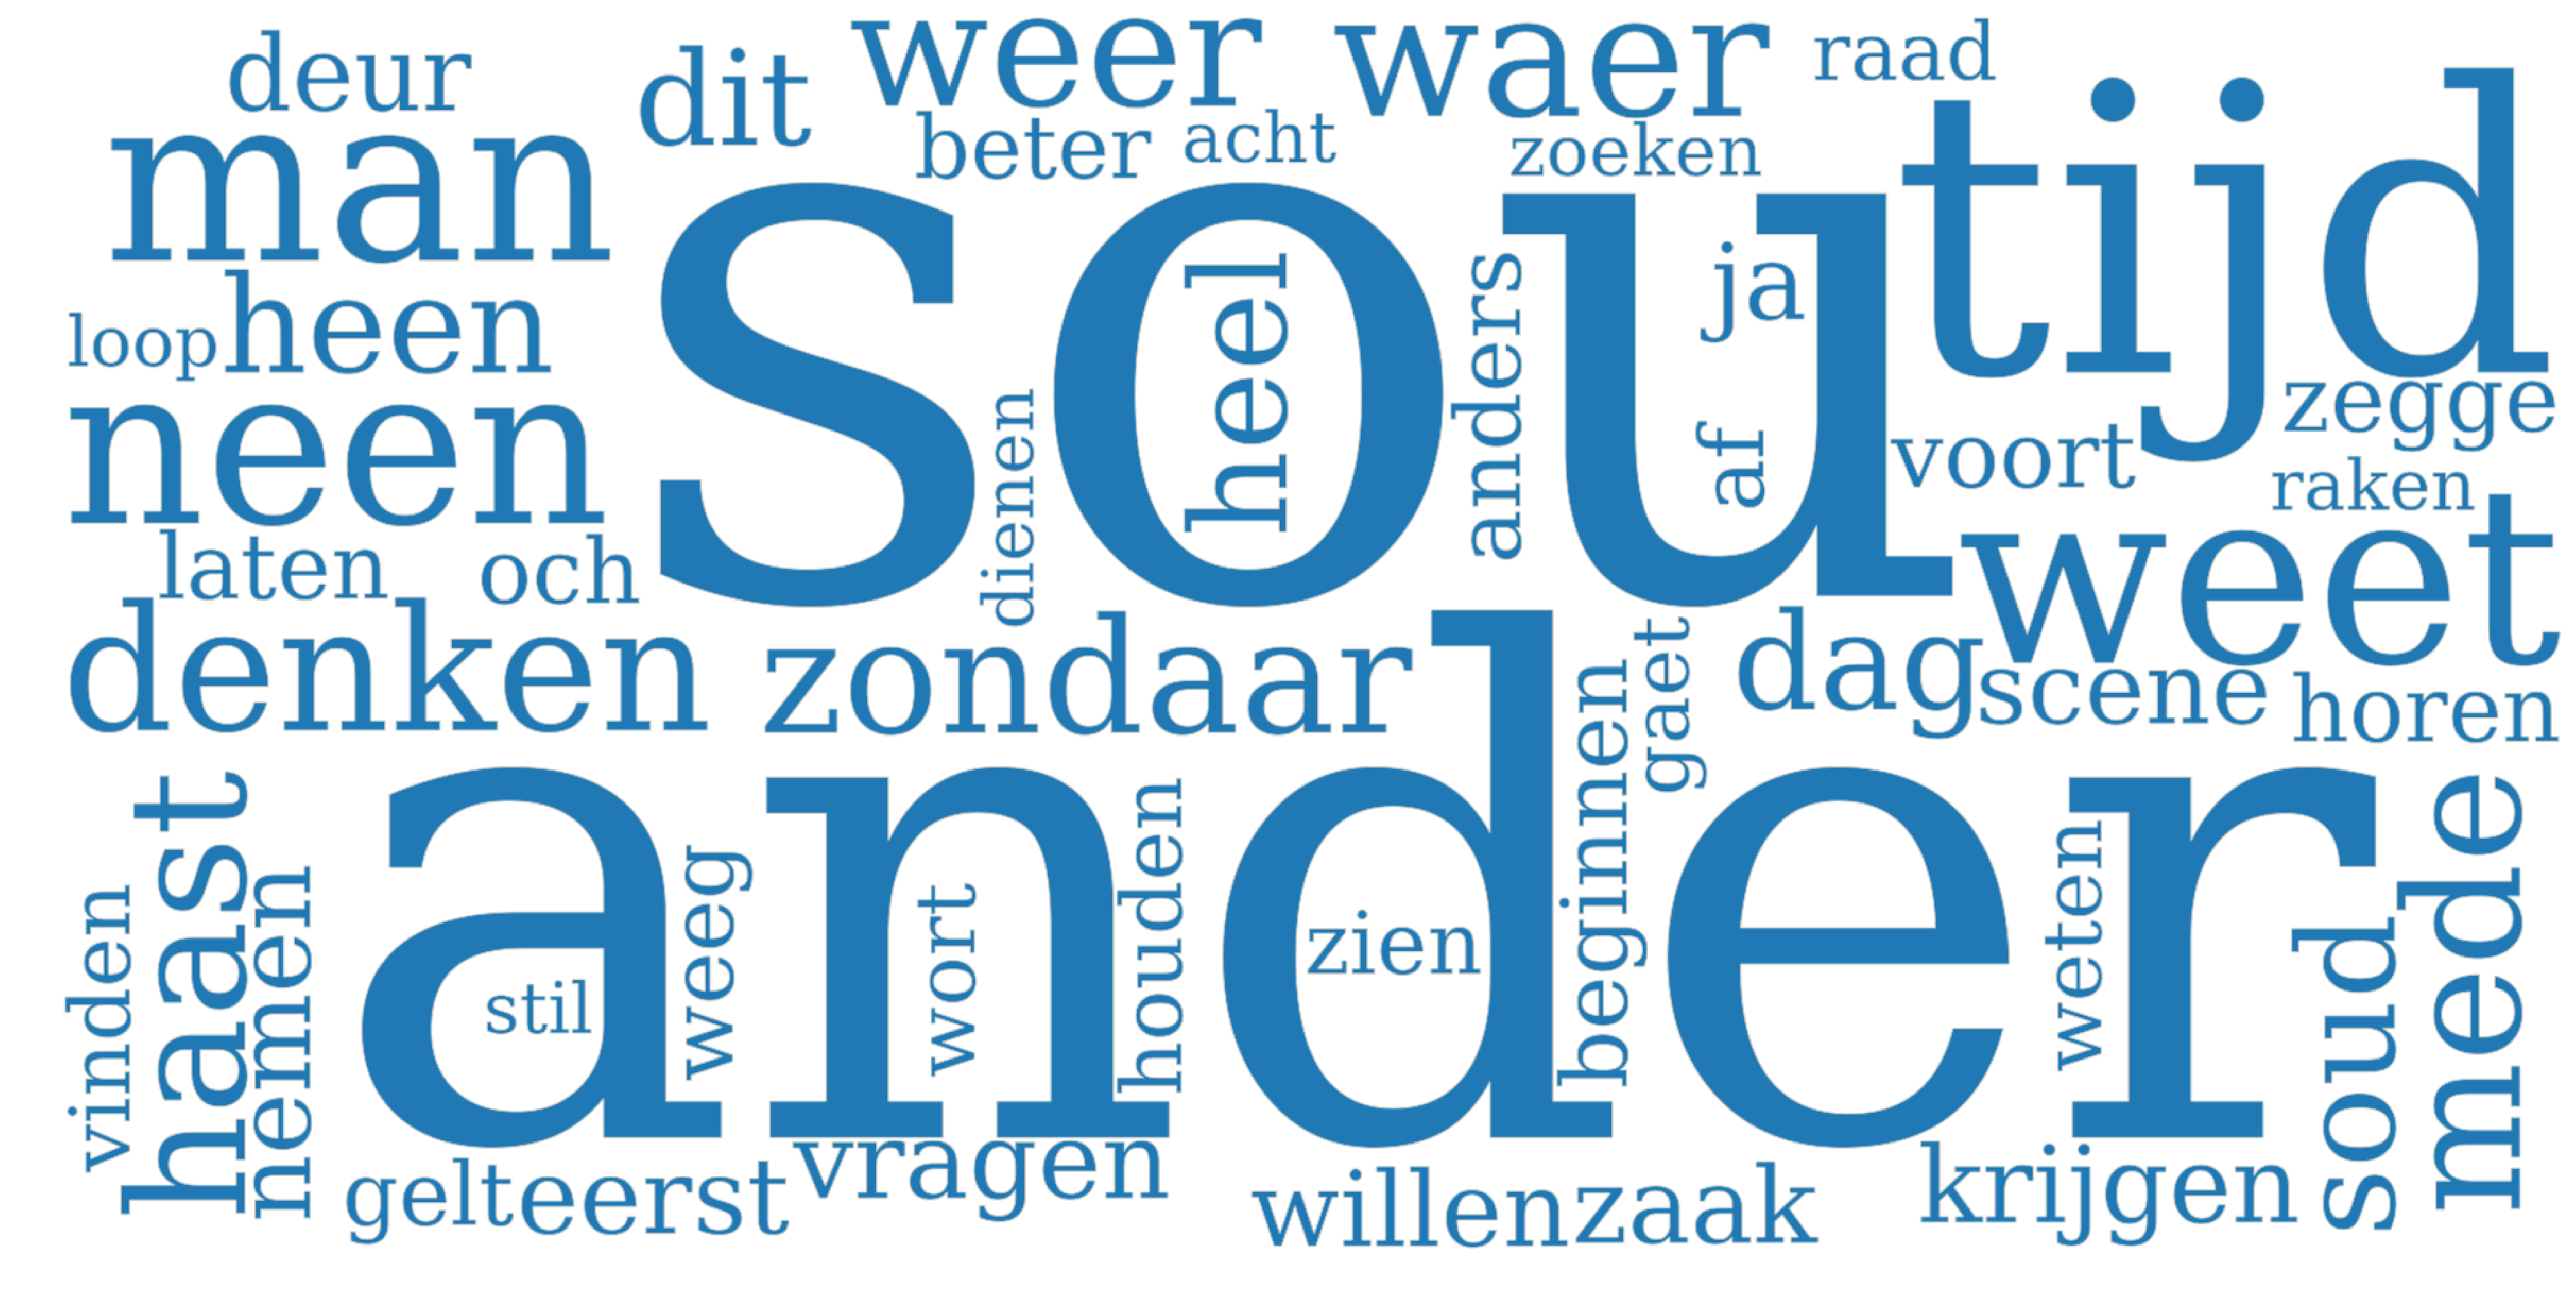
\includegraphics[width=\linewidth]{INL_topic38}
		\caption{\textit{???} (38, INL)}
		\label{fig:Topic38INL}
		\vspace{4ex}
	\end{minipage}%%
	\begin{minipage}[c]{0.48\linewidth}
		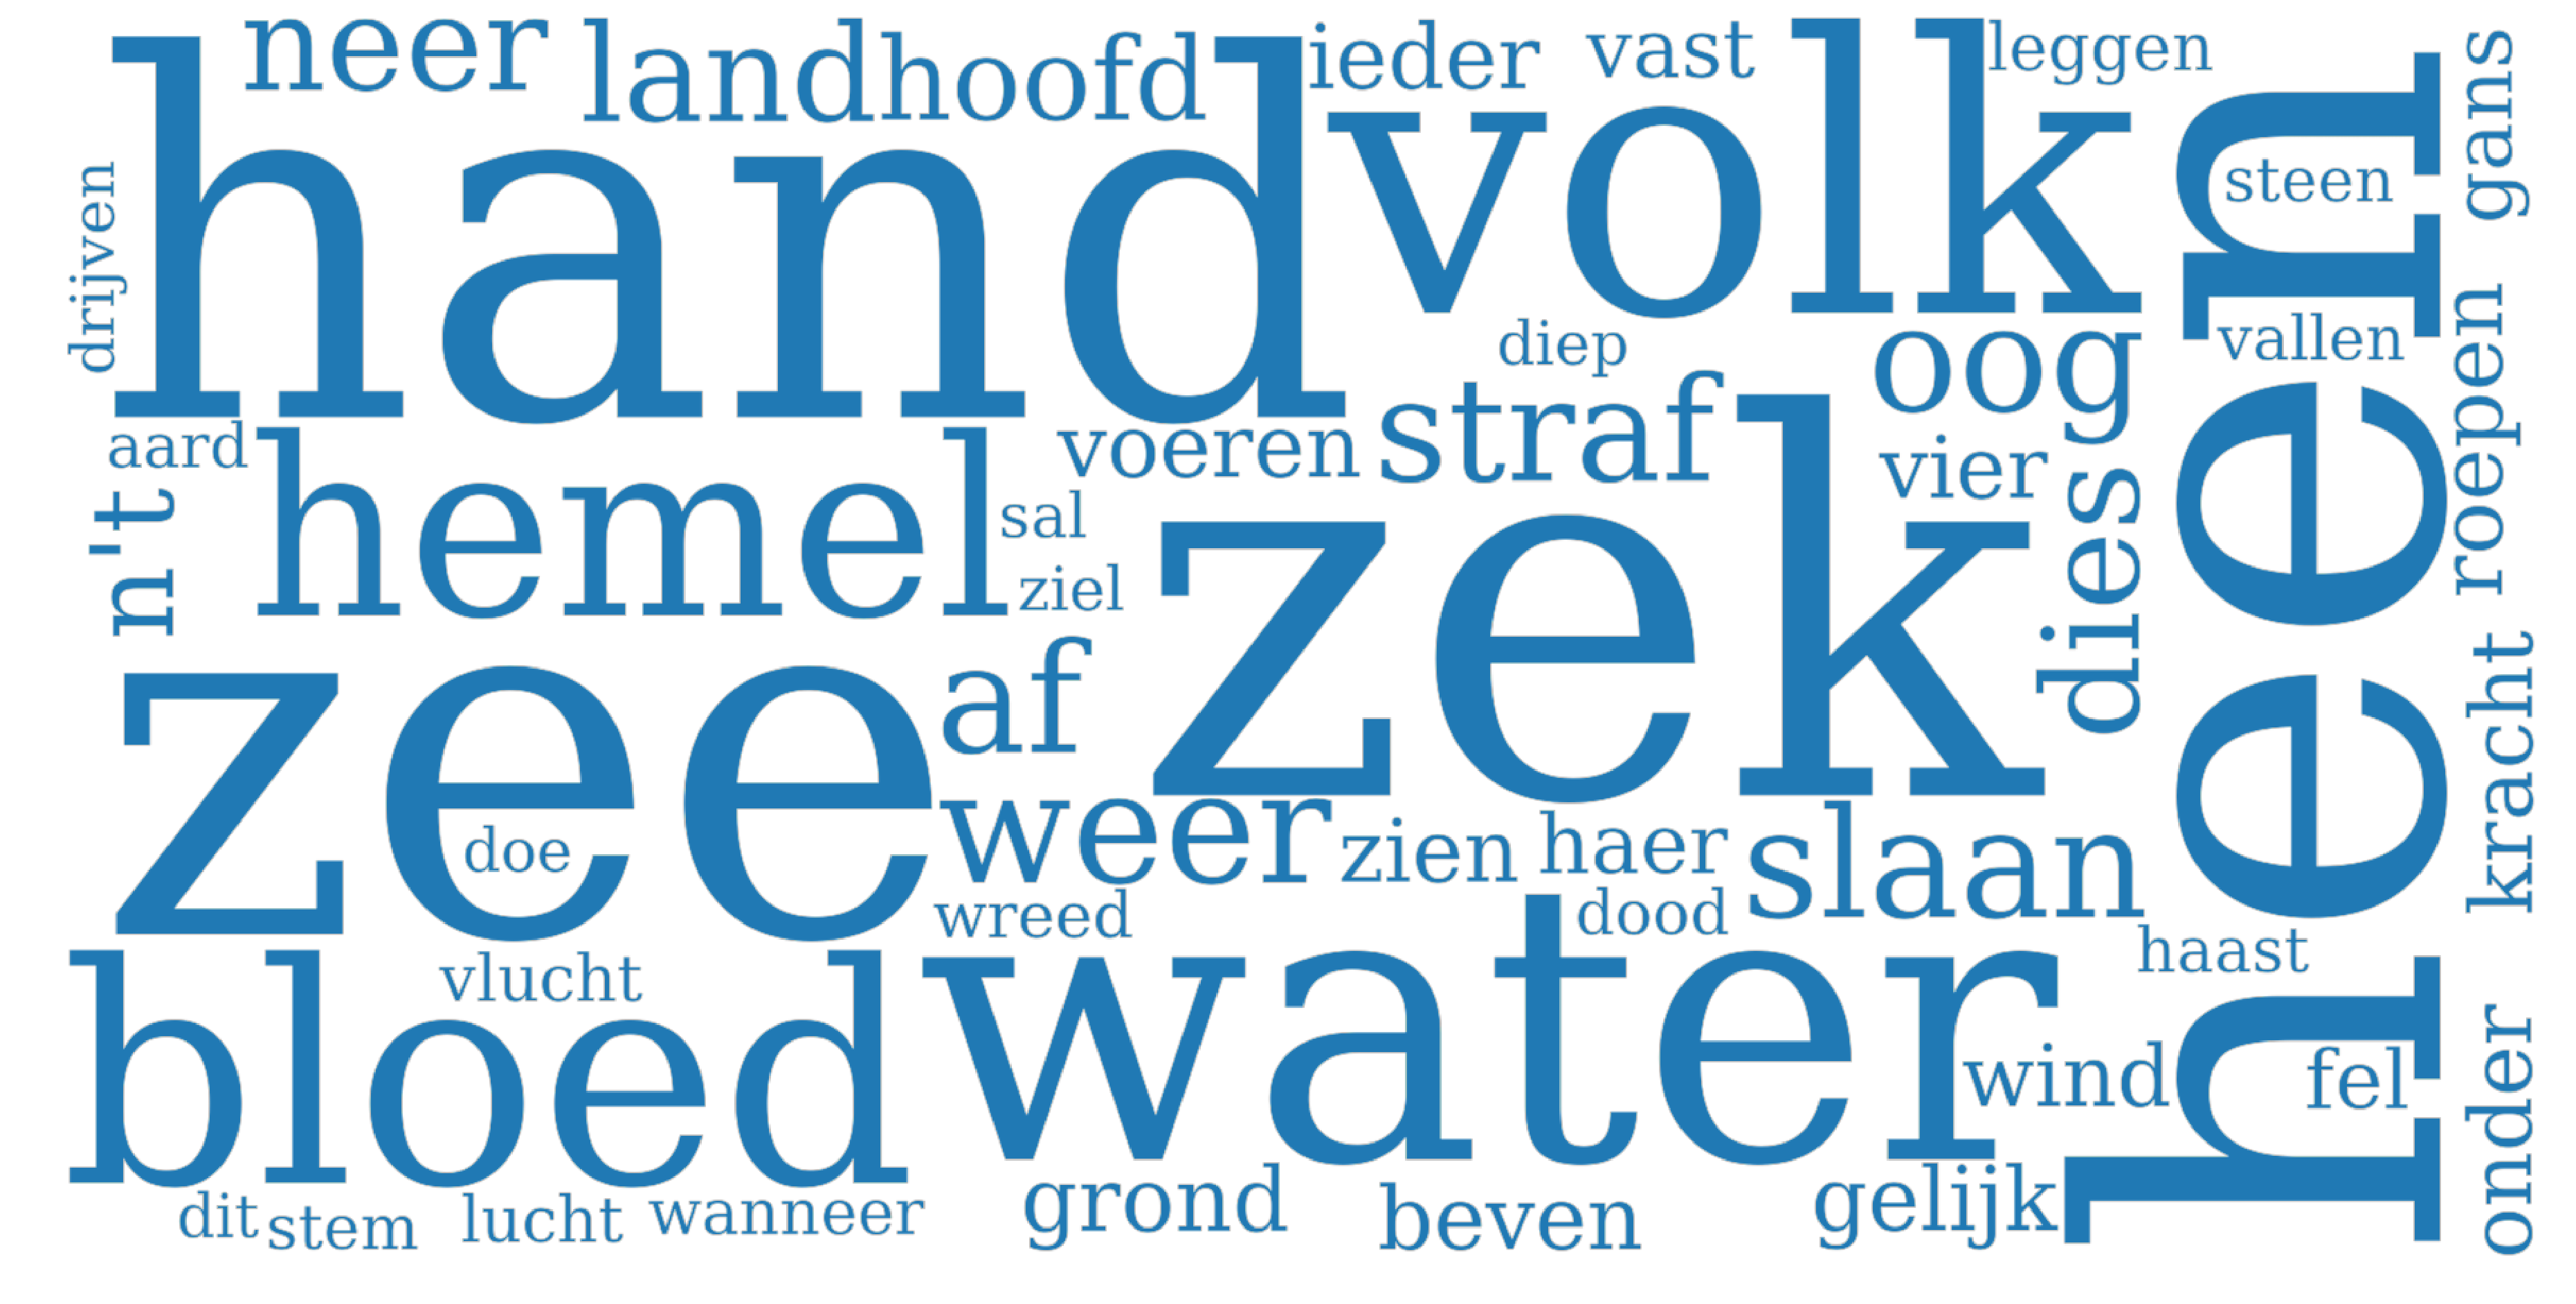
\includegraphics[width=\linewidth]{INL_topic15}
		\caption{\textit{???} (15, INL)}
		\label{fig:Topic15INL}
		\vspace{4ex}
	\end{minipage}%%
\end{figure}

\begin{table}
	\begin{minipage}{0.5\textwidth}
		\begin{tabular}{ccl}
			\toprule
			Topic & Songs & Subject \\
			\midrule
			24             &  1337 & sadness  \\
			39             &  1113 & heart \& soul \\
			21             &   965 & religion \& Christ \\
			4              &   952 & man \& life \\
			25             &   910 & live \& love \\
			38             &   903 & ??? \\
			16             &   862 & religion \\
			26             &   859 & love \\
			33             &   807 & religion \\
			15             &   759 & ??? \\
			30             &   671 & religion \& happiness \\
			42             &   663 & religion \& passion \\
			37             &   576 & physical love \\
			20             &   550 & bucolic songs \\
			22             &   510 & religion \& love \\
			2              &   496 & family??? \\
			11             &   492 & persons \\
			34             &   462 & religion \\
			6              &   459 &  drinking \\
			9              &   452 & live \& die \\
			3              &   430 & religion \\
			8              &   425 & religion \\
			41             &   407 & Christmas \\
			43             &   394 & marriage \\
			29             &   369 & religion \\
			\vdots & \vdots & \vdots \\
			\bottomrule
		\end{tabular}
	\end{minipage} \hfill
	\begin{minipage}{0.5\textwidth}
		\begin{tabular}{|ccl}
			\toprule
			Topic & Songs & Subject  \\
			\midrule
			\vdots & \vdots & \vdots \\
			10             &   354 & beauty??? \\
			28             &   351 & old spelling \\
			40             &   332 & religion \& passion \\
			47             &   330 & religion \\
			45             &   316 & love  \\
			5              &   267 &  truth \& lie \\
			49             &   260 & nature \\
			23             &   256 & religion \& positive emotions \\
			19             &   252 & ??? \\
			32             &   249 & sea \\
			18             &   246 & mother \& father \\
			14             &   241 & nation \& country \\
			13             &   230 & church \\
			17             &   224 & religion \\
			48             &   218 & enemy \\
			7              &   211 & Old Testament \\
			27             &   176 & happiness \& singing \\
			46             &   156 & sun \\
			0              &   147 & eternal life \\
			31             &   144 & French \\
			44             &   128 & mythology \\
			1              &   121 & possessives \\
			12             &   113 & German \\
			36             &    94 & trash \\
			35             &    58 & solfège \\
			\bottomrule
		\end{tabular}
	\end{minipage}
\caption{Dominant topics in INL-normalized corpus (\textit{n} = 22,297)}
\label{table:DomTopINL}
\end{table}

A visualization with \texttt{pyLDAvis} actually confirms these doubts. Figure~\ref{fig:pyLDAvisINL} shows that, instead of an improved scatter plot compared to Figure~\ref{fig:pyLDAvisOriginal}, the topics overlap just as much. It even seems that the bubbles, except the four in the bottom right quadrant, are clustered closer to each other. This also explains the difficulty to assign a specific subject to many topics. I can therefore conclude that a normalization tool as raw and straightforward as the INL-tool does not improve further results of textual analysis. The third option is building topics from the corpus that is normalized with the VARD2-tool.

\begin{figure}[hbt!]
	\centering
	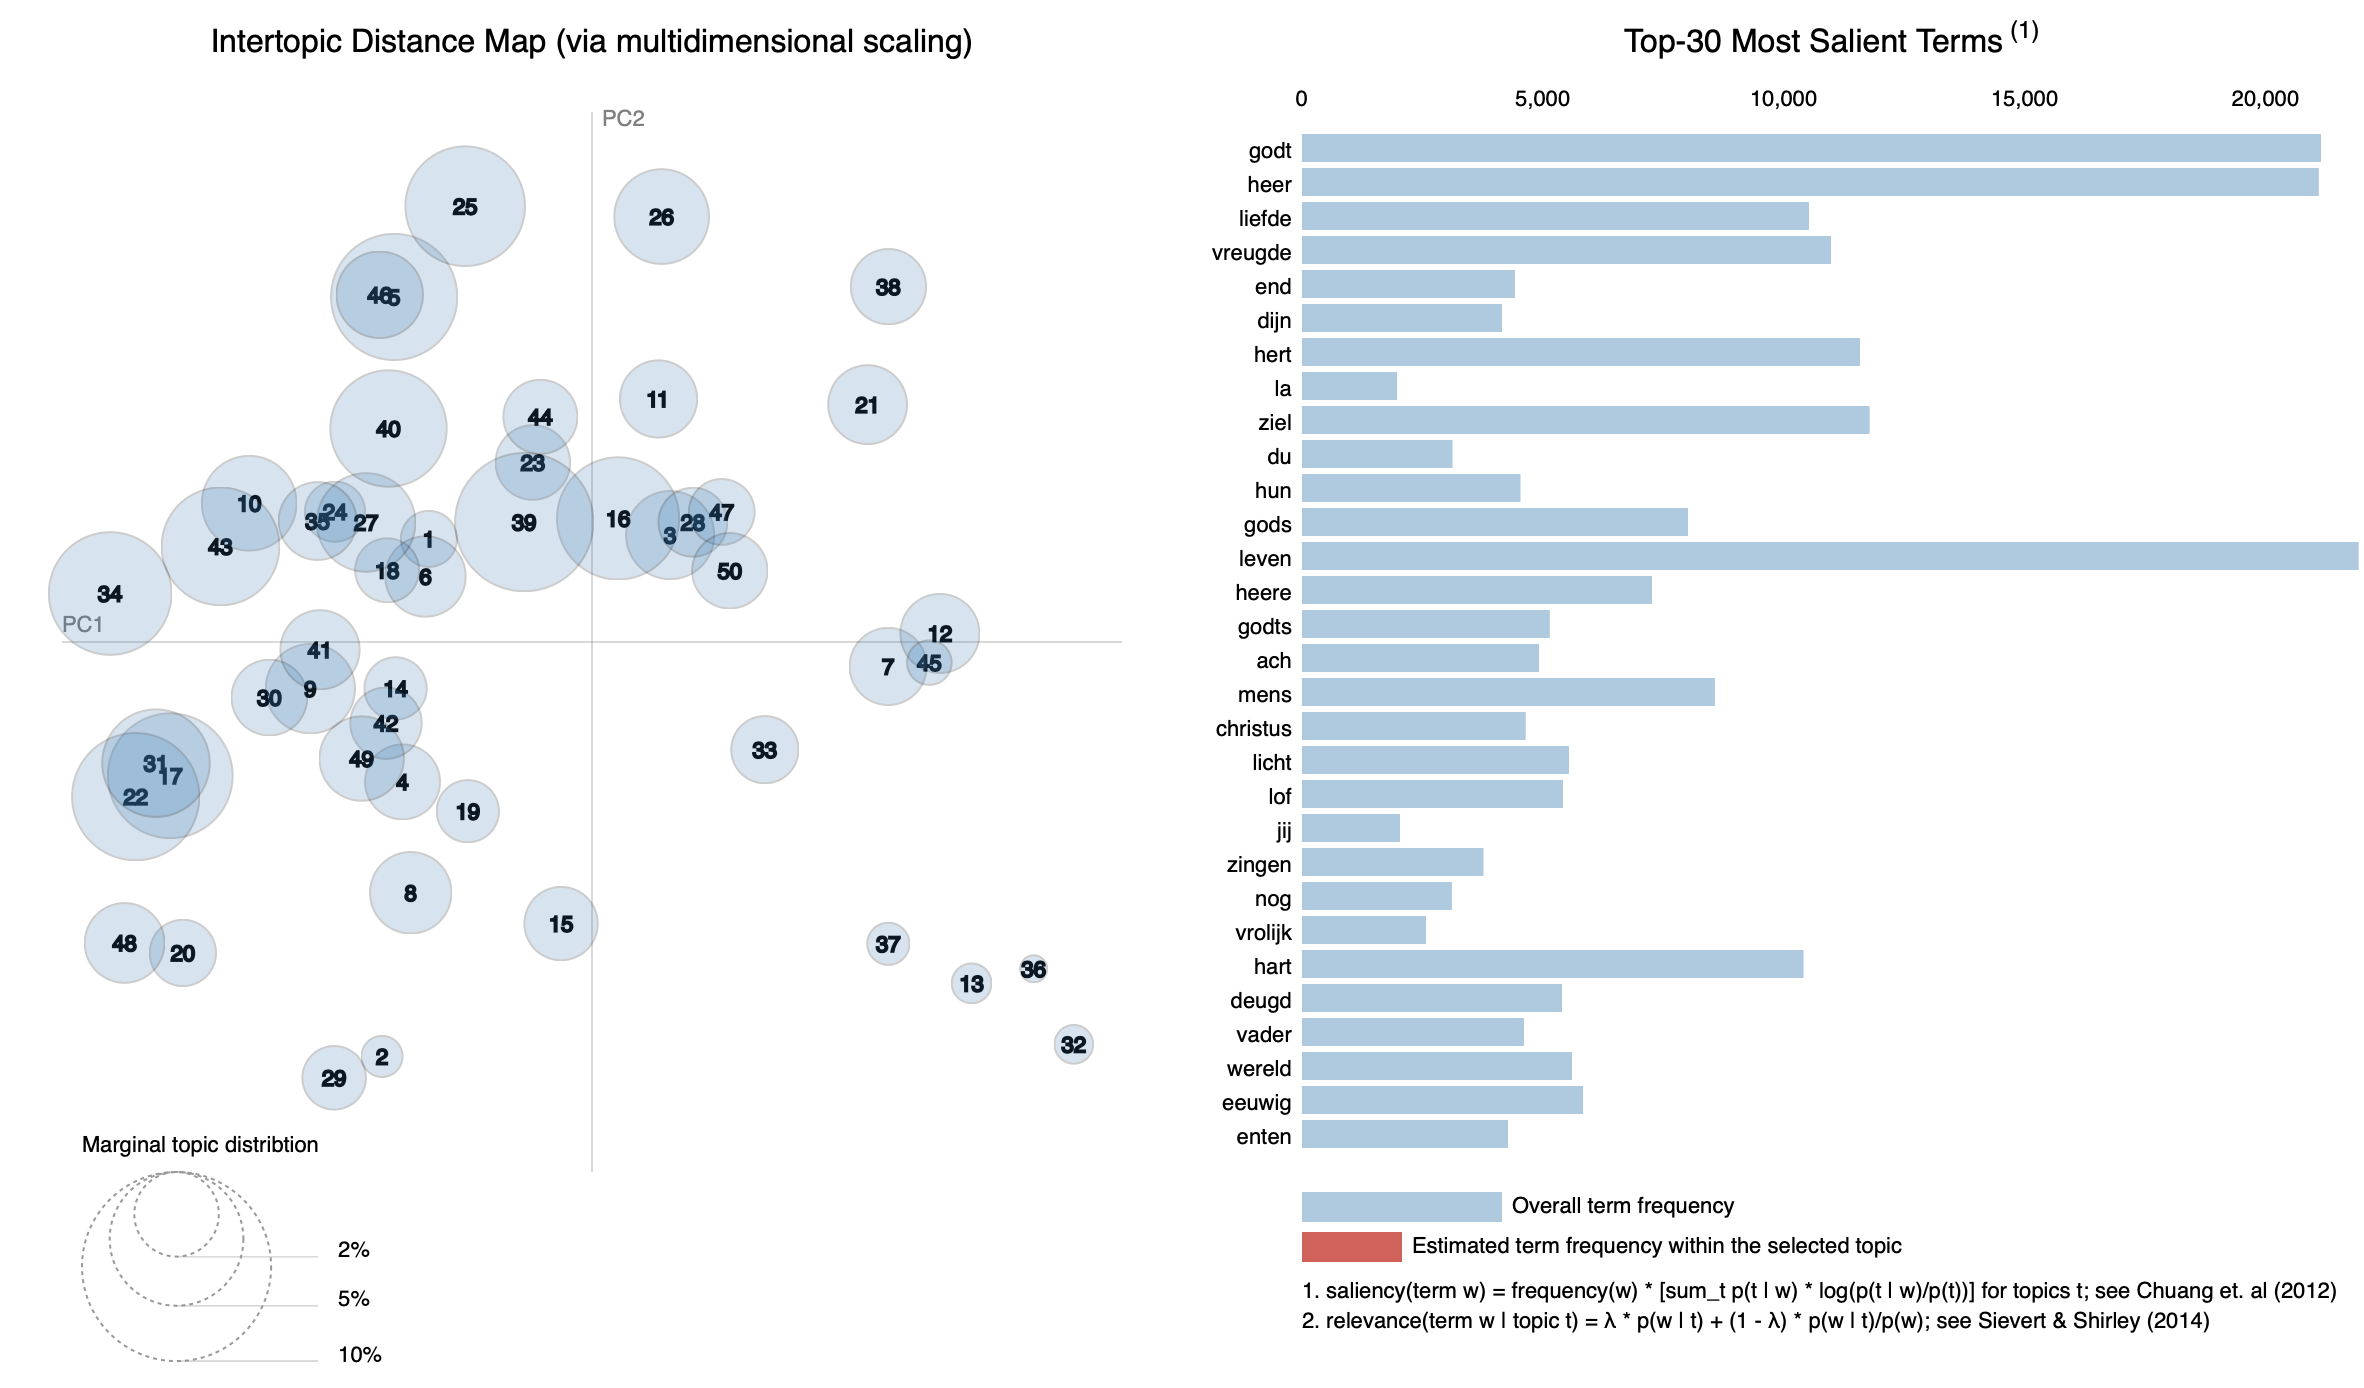
\includegraphics[scale=0.3]{INL_pyLDAvis}
	\caption{Visualization of topics in the INL-normalized corpus with \texttt{pyLDAvis}}
	\label{fig:pyLDAvisINL}
\end{figure}

\subsection{VARD2-normalized corpus}
At first there were 194,159 tokens in the dictionary that was built from the VARD2-normalized corpus. After eliminating 117,045 tokens with \texttt{no\_below = 2}, 77,114 tokens remained. For the final time I let the tool compose 50 topics. The coherence score of the built model was 0.4962, which is higher than the score of the model built from the INL-normalized corpus. The visualization made with \texttt{pyLDAvis} immediately shows that this topic model obtained better results than the one built in the previous paragraph. The bubbles are more evenly scattered throughout the chart, and less bubbles overlap with each other. This creates the expectation that the subjects of the topics made from this version of the corpus, are easier to assign. Below I discuss some topics and how I assigned a subject to them. The results are stored in Table~\ref{table:DomTopVARD2}. Besides, I examined for each topic which song represented this topic at best, in other words, which song had the highest contribution to that specific topic, using the following code: 

\begin{lstlisting}
song_topic_highest_contribution = pd.DataFrame()
song_topics_outdf_grpd = dominant_topics.groupby("dominant_topic")

for i, grp in song_topics_outdf_grpd:
song_topic_highest_contribution = pd.concat([song_topic_highest_contribution, grp.sort_values(["perc_contribution"], ascending=[0]).head(1)], axis=0)

song_topic_highest_contribution.reset_index(drop=True, inplace=True)
song_topic_highest_contribution.columns = ["id", "topic", "perc_contribution"]
\end{lstlisting}

To topic 28 (Figure~\ref{fig:topic28VARD2}), the most prevalent topic in this corpus, I assigned the topic \textit{religion \& intangibility}, since the words in this topic were mainly about the intangible aspects of religion, such as \enquote{ziel}, \enquote{geest} and \enquote{eeuwig}. The song that represents this topic the most, is a sung version of the Lord's prayer (\texttt{id} = 118423), of which I quote the first three stanzas below:

\begin{quote}
	 ONse Vader in Hemelrijck,\\
	Die ons heet kinders al gelijck,\\
	En wilt dat wy u roepen aen,\\
	Als wy met node zijn bevaen:\\
	Geeft dat niet bidt alleen den mondt,\\
	Maer dat het gae uyt 's herten gront.\\
	
	Geheyligt uwen name zy,\\
	U woordt ongevalscht blijv' ons by:\\
	Dat wy oock leven heyliglijck,\\
	Na uwen name weerdiglijck,\\
	Behoet ons Heer, voor valsche leer,\\
	Dat 't arm vervoerde volck bekeer.\\
	
	U Koninghrijck koom', Heere goet,\\
	Hier en hier na. Den trooster soet\\
	Geeft ons dien Chrisius ons toesey\\
	Met zijn gaven menigerley:\\
	Breeckt Satans tooren ende macht;\\
	Voor zijn ergheyt u Kercke wacht.
\end{quote}

\noindent It is understandable that this particular song represents this topic: the Lord's Prayer commemorates specifically the intangible aspects of the christian belief. Topic 27 (Figure~\ref{fig:topic27VARD2}), to which I assigned \textit{world \& money}, is represented at best by this song, dated from 1645 (\texttt{id} = 3207):

\begin{quote}
	ACh! snoode overdaedt,\\
	Vrouw-voedtster van de vuyle dartelheyt,\\
	Oorsaeck van alle quaedt,\\
	Of immers 't geen den wegh daer toe bereyt:\\
	V weelde baert veel onghemack,\\
	En Wellust is een lastigh pack.\\
	
	Die stil en wel te vre'en\\
	Met redelijck behoef is wel vernoegh,\\
	En gaet in vrede heen,\\
	En is gherust hoe 't Godt de Heere voeght:\\
	Die isser vry veel beter an;\\
	Ghenoegh, dat maeckt een deftigh man.\\
	
	Ghnoegh heeft overvloedt,\\
	Schoon dat sen kasjes ledigh zijn van geldt;\\
	Ghenoegh heeft schat en goedt,\\
	Ghenoegh is nimmermeer om Goudt ontsteldt:\\
	Hy leeft gherust die wynigh heeft,\\
	En by sijn weynigh eerlijck leeft.
\end{quote}

\begin{figure}[hbt!]
	\centering
	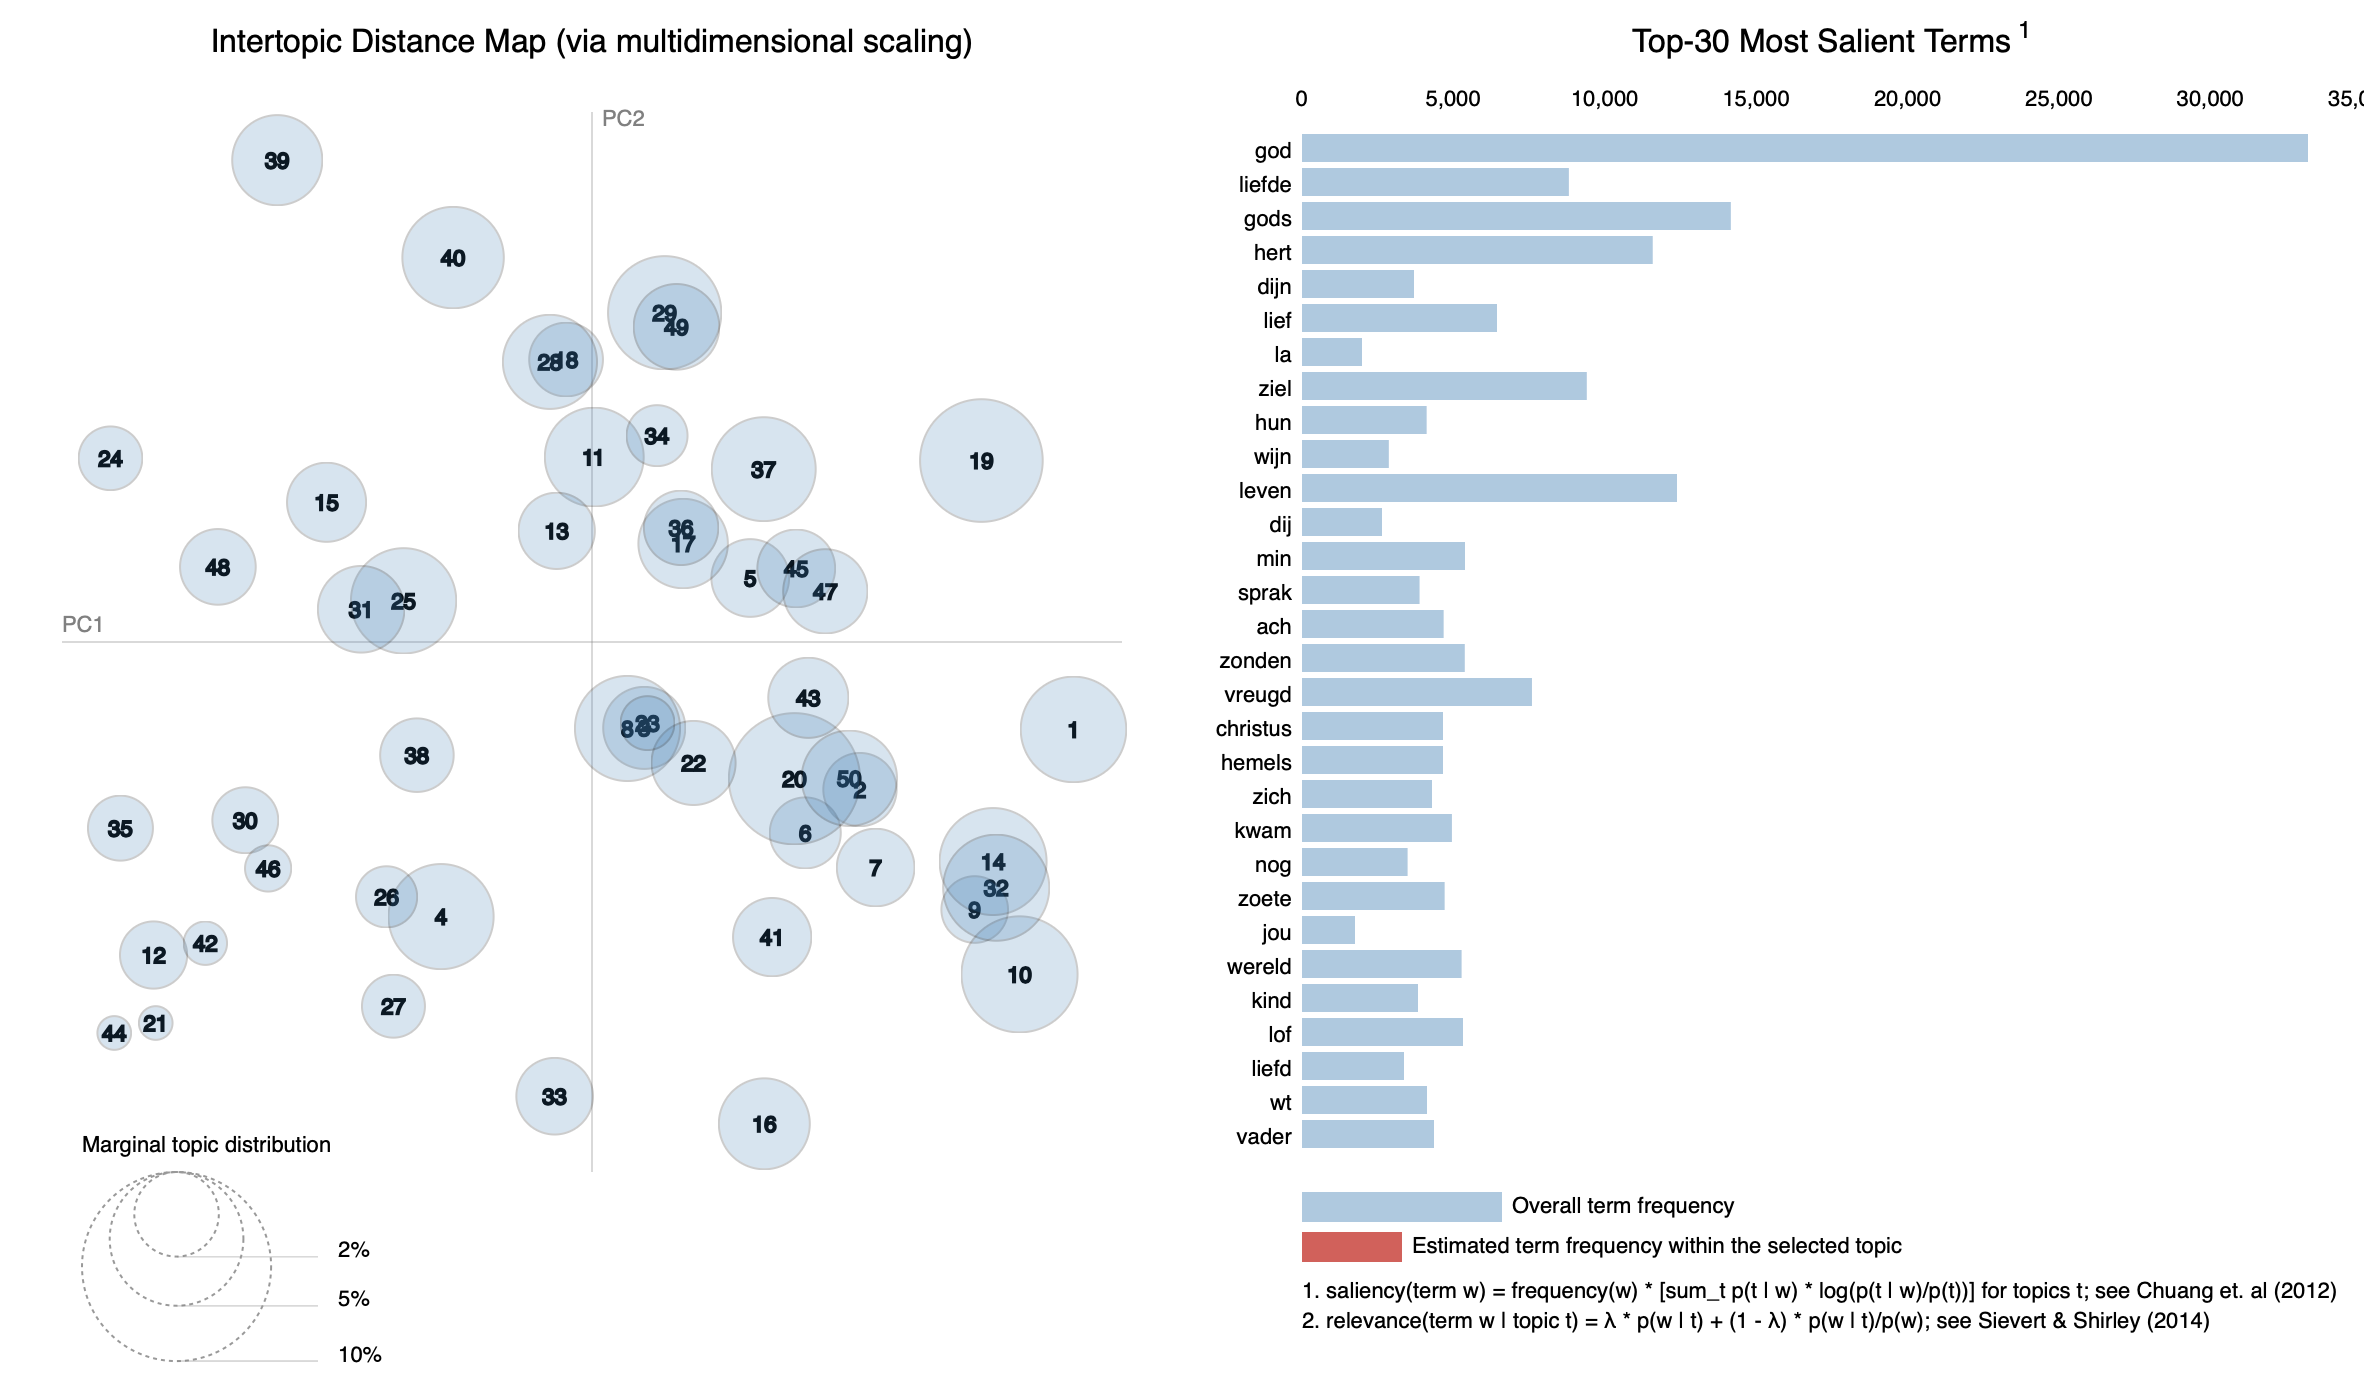
\includegraphics[scale=0.3]{VARD2_pyLDAvis}
	\caption{Visualization of topics in the VARD2-normalized corpus with \texttt{pyLDAvis}}
	\label{fig:pyLDAvisVARD2}
\end{figure}

\noindent Though the song contains various metaphorical phrases, such as \enquote{vrouw-voedster van de vuyle dartelheyt}, \enquote{oorsaeck van alle quadth}, \enquote{Wellust is een lastigh pack}, the song is still recognized as a song on wealth and soberness.

\begin{table}
	\begin{minipage}{0.5\textwidth}
		\begin{tabular}{ccl}
			\toprule
			Topic & Songs & Subject \\
			\midrule
			28             &  1151 & intangible religion \\
			39             &  1094 & love \& sadness \\
			38             &  1092 & love \& happiness \\
			18             &   878 & religion \\
			9              &   815 & religion \& old spelling \\
			0              &   756 & religion \& life \\
			24             &   618 & rejection \\
			2              &   591 & love \& tragedy \\
			13             &   591 & religion \\
			27             &   532 & world \& money \\
			6              &   521 & possessives \\
			31             &   518 & religion \\
			4              &   512 & religion \& happiness \\
			30             &   506 & love \\
			7              &   499 & God \& enemy \\
			14             &   498 & myth \& beauty \\
			21             &   477 & love \& happiness \\
			47             &   477 & bucolic songs \\
			44             &   465 & religion \& virtue \\
			40             &   464 & religion \& Jesus\\
			19             &   452 & verbs \\
			36             &   436 & religion \\
			49             &   432 & God \& country \\
			5              &   427 & Christmas \\
			12             &   422 & marriage \\
			\vdots & \vdots & \vdots \\
			\bottomrule
		\end{tabular}
	\end{minipage} \hfill
	\begin{minipage}{0.5\textwidth}
		\begin{tabular}{|ccl}
			\toprule
			Topic & Songs & Subject  \\
			\midrule
			\vdots & \vdots & \vdots \\						
			16             &   406 & good \& evil \\
			3              &   395 & verbs \\
			1              &   390 & religion \& Mary \\
			35             &   388 & religion \\
			46             &   386 & earthly life \\
			10             &   383 & suffer \& sadness \\
			29             &   378 & drinking \\
			48             &   377 & love \\
			23             &   355 & physical love \\
			34             &   351 & seducing \\
			32             &   340 & nation \& country \\
			42             &   339 & cross \& passion \\
			37             &   280 & nature \\
			8              &   268 & godly life \\
			11             &   253 & entertainment \\
			26             &   250 & money \& work \\
			15             &   248 & Old Testament \\
			17             &   244 & heaven \\
			22             &   227 & church \\
			25             &   201 & sea \\
			33             &   187 & ??? \\
			45             &   140 & trash \\
			41             &   124 & German \\
			43             &    97 & French \\
			20             &    66 & solfège \\
			\bottomrule
		\end{tabular}
	\end{minipage}
	\caption{Dominant topics in VARD2-normalized corpus (\textit{n} = 22,297)}
	\label{table:DomTopVARD2}
\end{table}

Topic 24 (Figure~\ref{fig:topic24VARD2}) is a remarkable one: I assigned the word \textit{rejection} to it. Several words, including the \enquote{weg}, \enquote{waarom} and especially the most prevalent \enquote{neen}, suggest that songs with this topic are about an unanswered love or the rejection of a lover. The song with this topic as its highest contribution shows this perfectly. Here I quote the first two stanzas (\texttt{id} = 10359):

\begin{quote}
	Ick ongheluckigh Vrijer,\\
	Hoe ben ick in de ly?\\
	Ick kan gheen Vrijster winnen,\\
	Hoe dapper dat ick vry,\\
	Sy achten 't maer voor grillen,\\
	't En klemt niet wat ick doe:\\
	Sal dit noch langher duuren,\\
	Ick wordt mijn leven moe.\\
	
	Ionghman waer toe dit klaghen,\\
	Ey! laet u grillen staen,\\
	'k En sagh van al mijn daghen\\
	Noyt sulcken vreemden Haen:\\
	Ghy reutelt en ghy rammelt,\\
	Als of ghy had' een gons,\\
	Ghy Bongioert selfs in jou Bocxsen,\\
	En leght die schult op ons.
\end{quote}

\noindent This song is a dialogue between Hylas and Phyllis. Hylas plays the role of an unlucky youngster who laments about his futile attempts in conquering a girl; Phyllis explains that girls do not like his rude approach. Another topic whose most representative song shows clearly the subjects of the songs belonging to this topic, is topic 32 on \textit{nation \& country} (Figure~\ref{fig:topic32VARD2}). The song with the highest contribution is a so called Geuzen song (\texttt{id} = 27769) from \textit{Een Nieu Geuse Lieden boecxken} (1578). Below the first three stanzas are quoted:

\begin{quote}
	Wel op, wel op Spangiaerden,\\
	Die nu in Brabant zijn,\\
	Hoe smaken u die ghebraden\\
	Daer toe den coelen wijn,\\
	Ghy moet naer Spangien met ghewelt,\\
	Sonder Paspoort, sonder gelt,\\
	Jochey, nu slaet dien Spangiaerts vry.\\
	
	In Brabant quamen sy dringhen\\
	Die Spaensche Jonckers wijs,\\
	Vlaendren wouden sy dwinghen,\\
	Die steden maecken prijs\\
	Of sy wolden hebben betaelt,\\
	Die leste penninck ongefaelt\\
	Jochey nu slaet de Spangiaerts vry.\\
	
	De Staten van den Lande,\\
	Die setten haer een dach,\\
	Wy sullen u wel betalen\\
	U Leeninghe corten af\\
	Soo moest ghy uyt den Lande gaen\\
	Die Spangiaerts riepen niet te verstaen\\
	Jochey, nu slaet de Spangiaerts vry.
\end{quote}

\begin{figure}
	\begin{minipage}[c]{0.48\linewidth}
		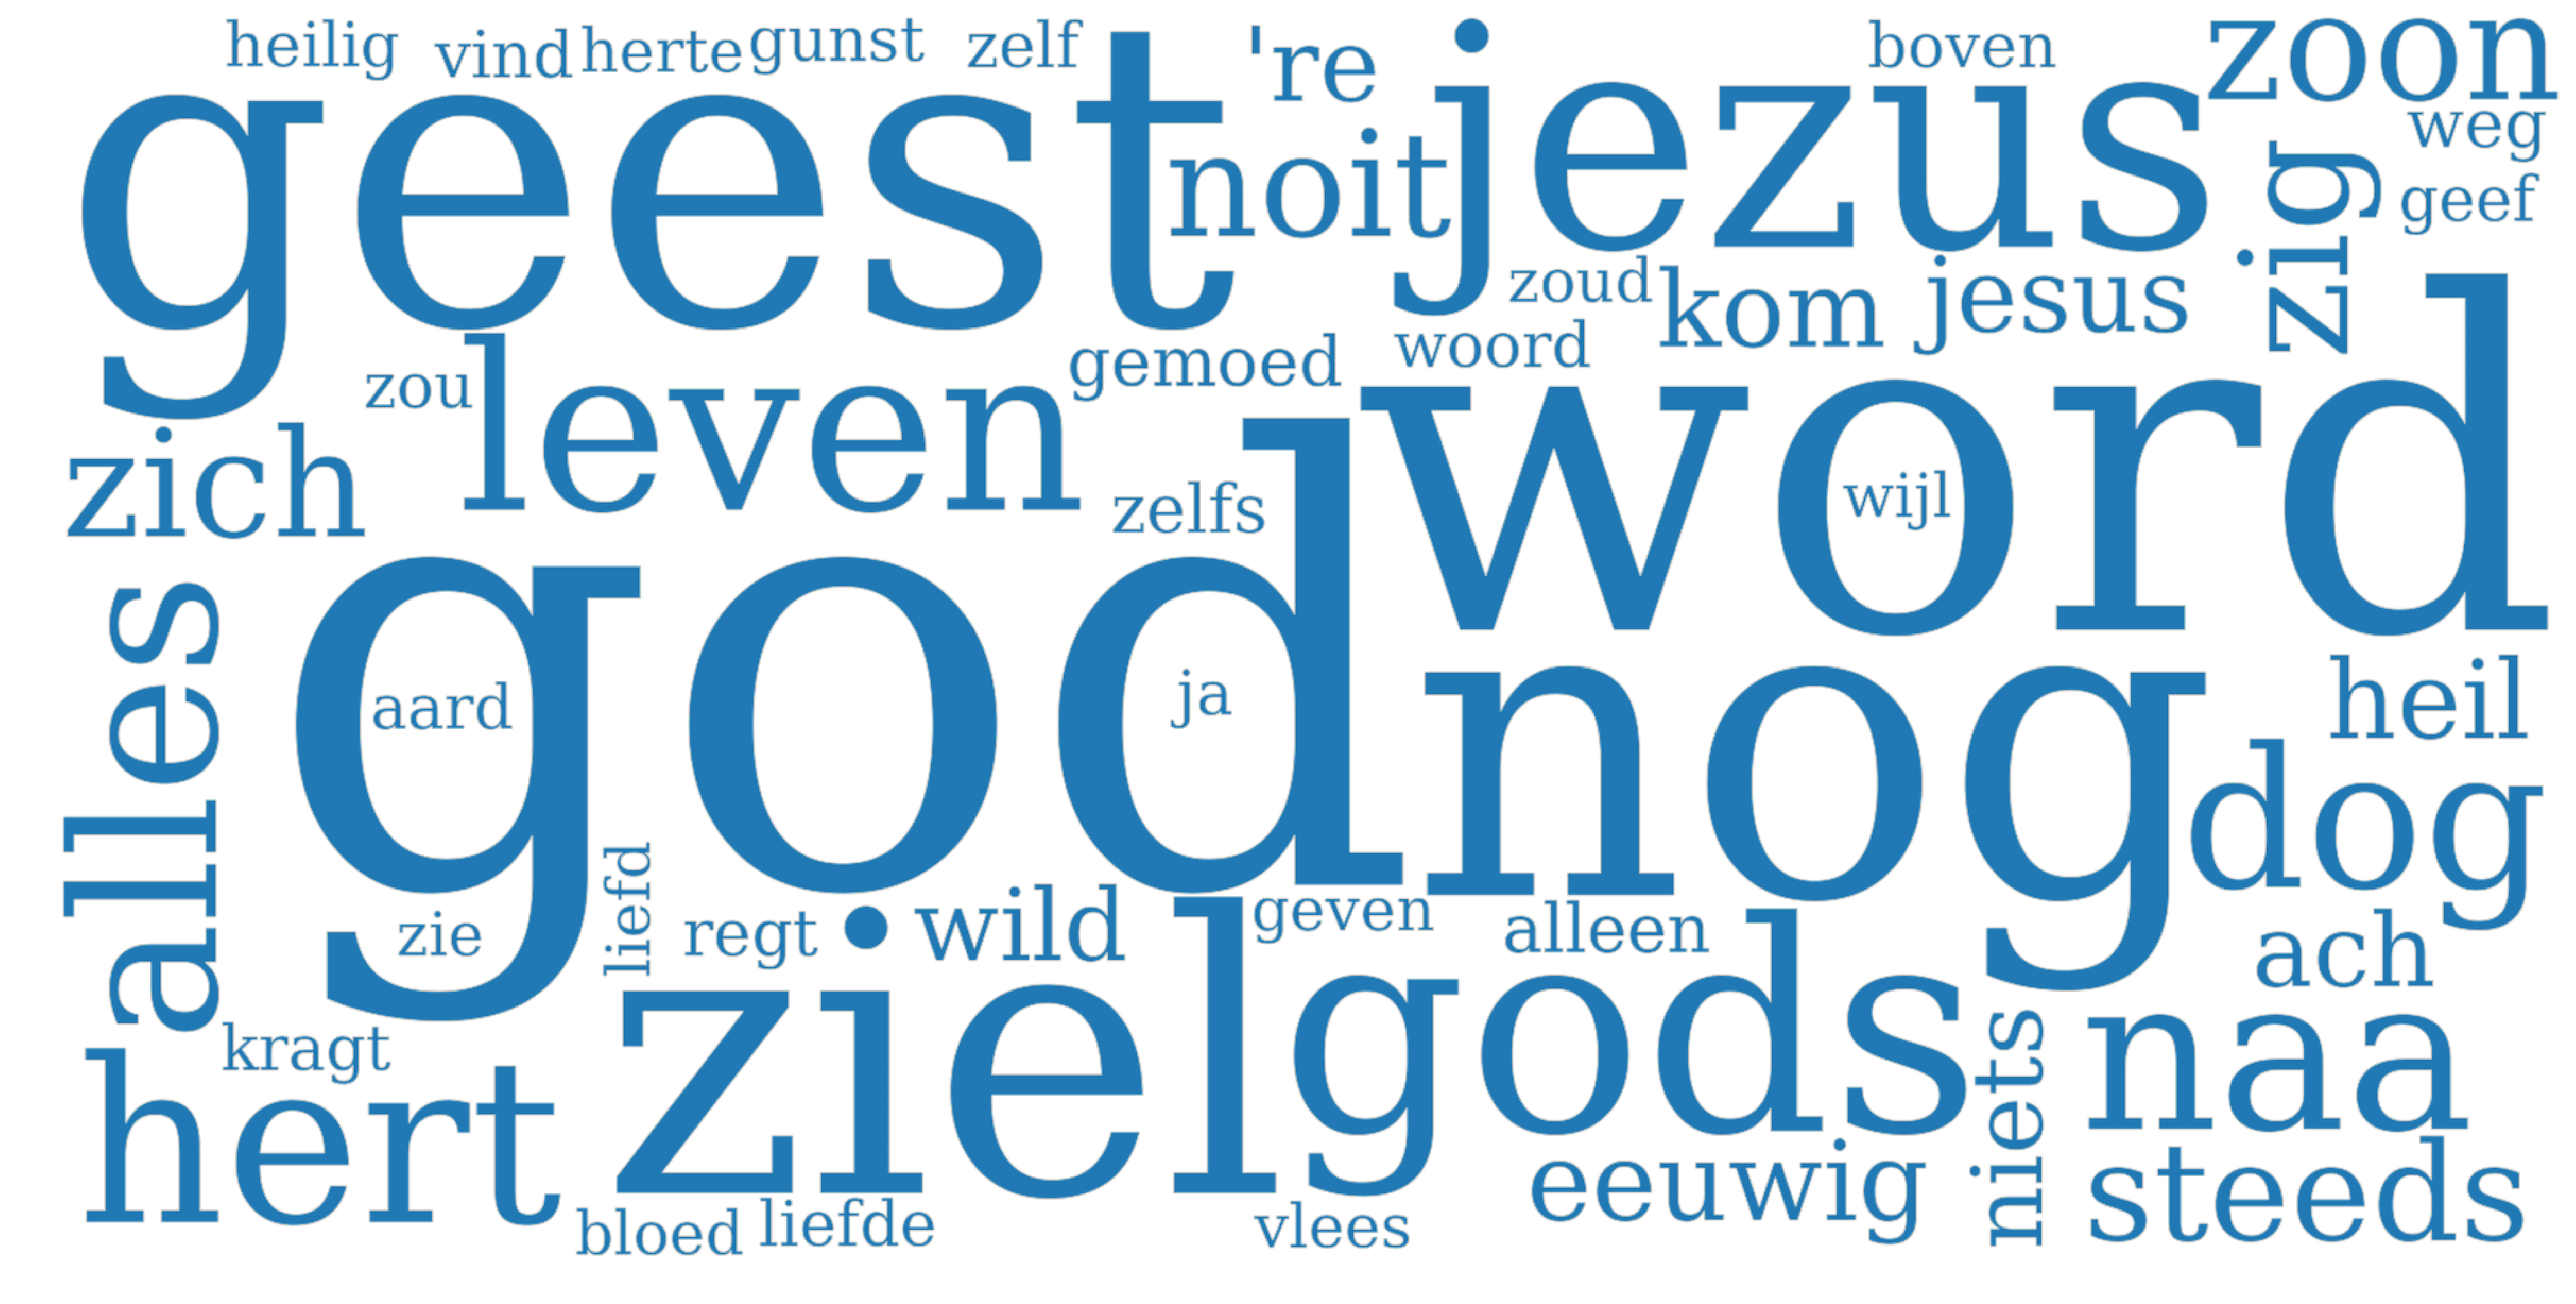
\includegraphics[width=\linewidth]{VARD2_topic28}
		\caption{\textit{religion \& intangibility} (28, VARD2)}
		\label{fig:topic28VARD2}
		\vspace{4ex}
	\end{minipage}%%
	\begin{minipage}[c]{0.48\linewidth}
		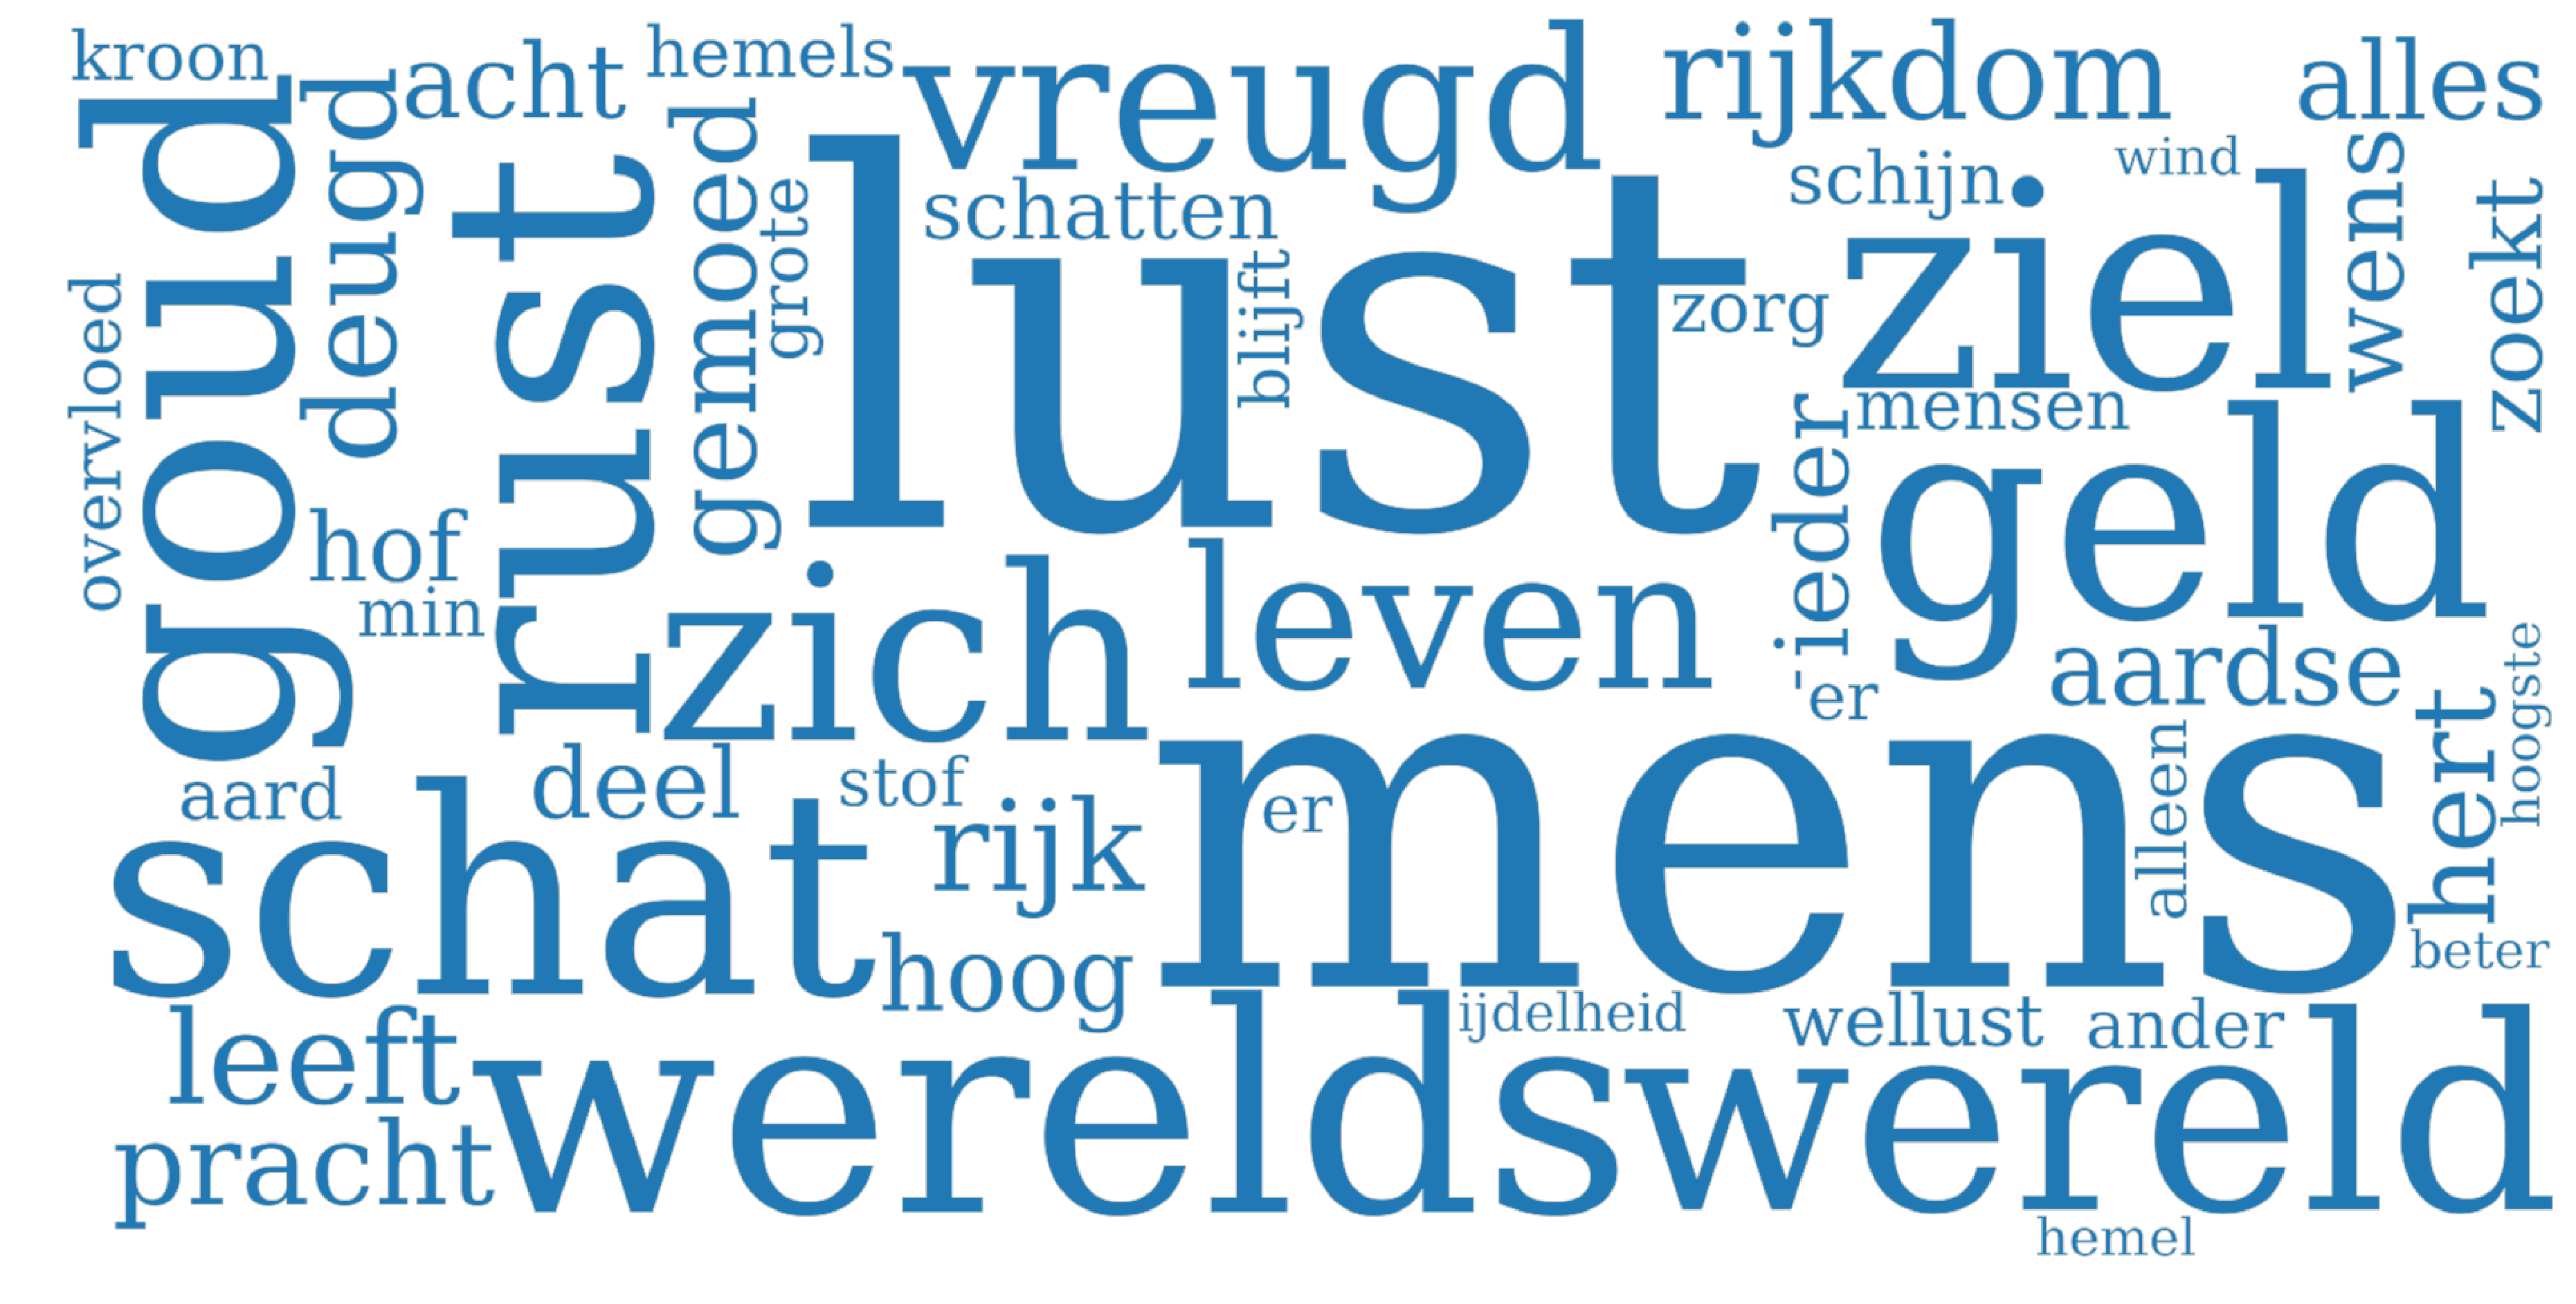
\includegraphics[width=\linewidth]{VARD2_topic27}
		\caption{\textit{world \& money} (27, VARD2)}
		\label{fig:topic27VARD2}
		\vspace{4ex}
	\end{minipage}%%
	\hfill
	\begin{minipage}[c]{0.48\linewidth}
		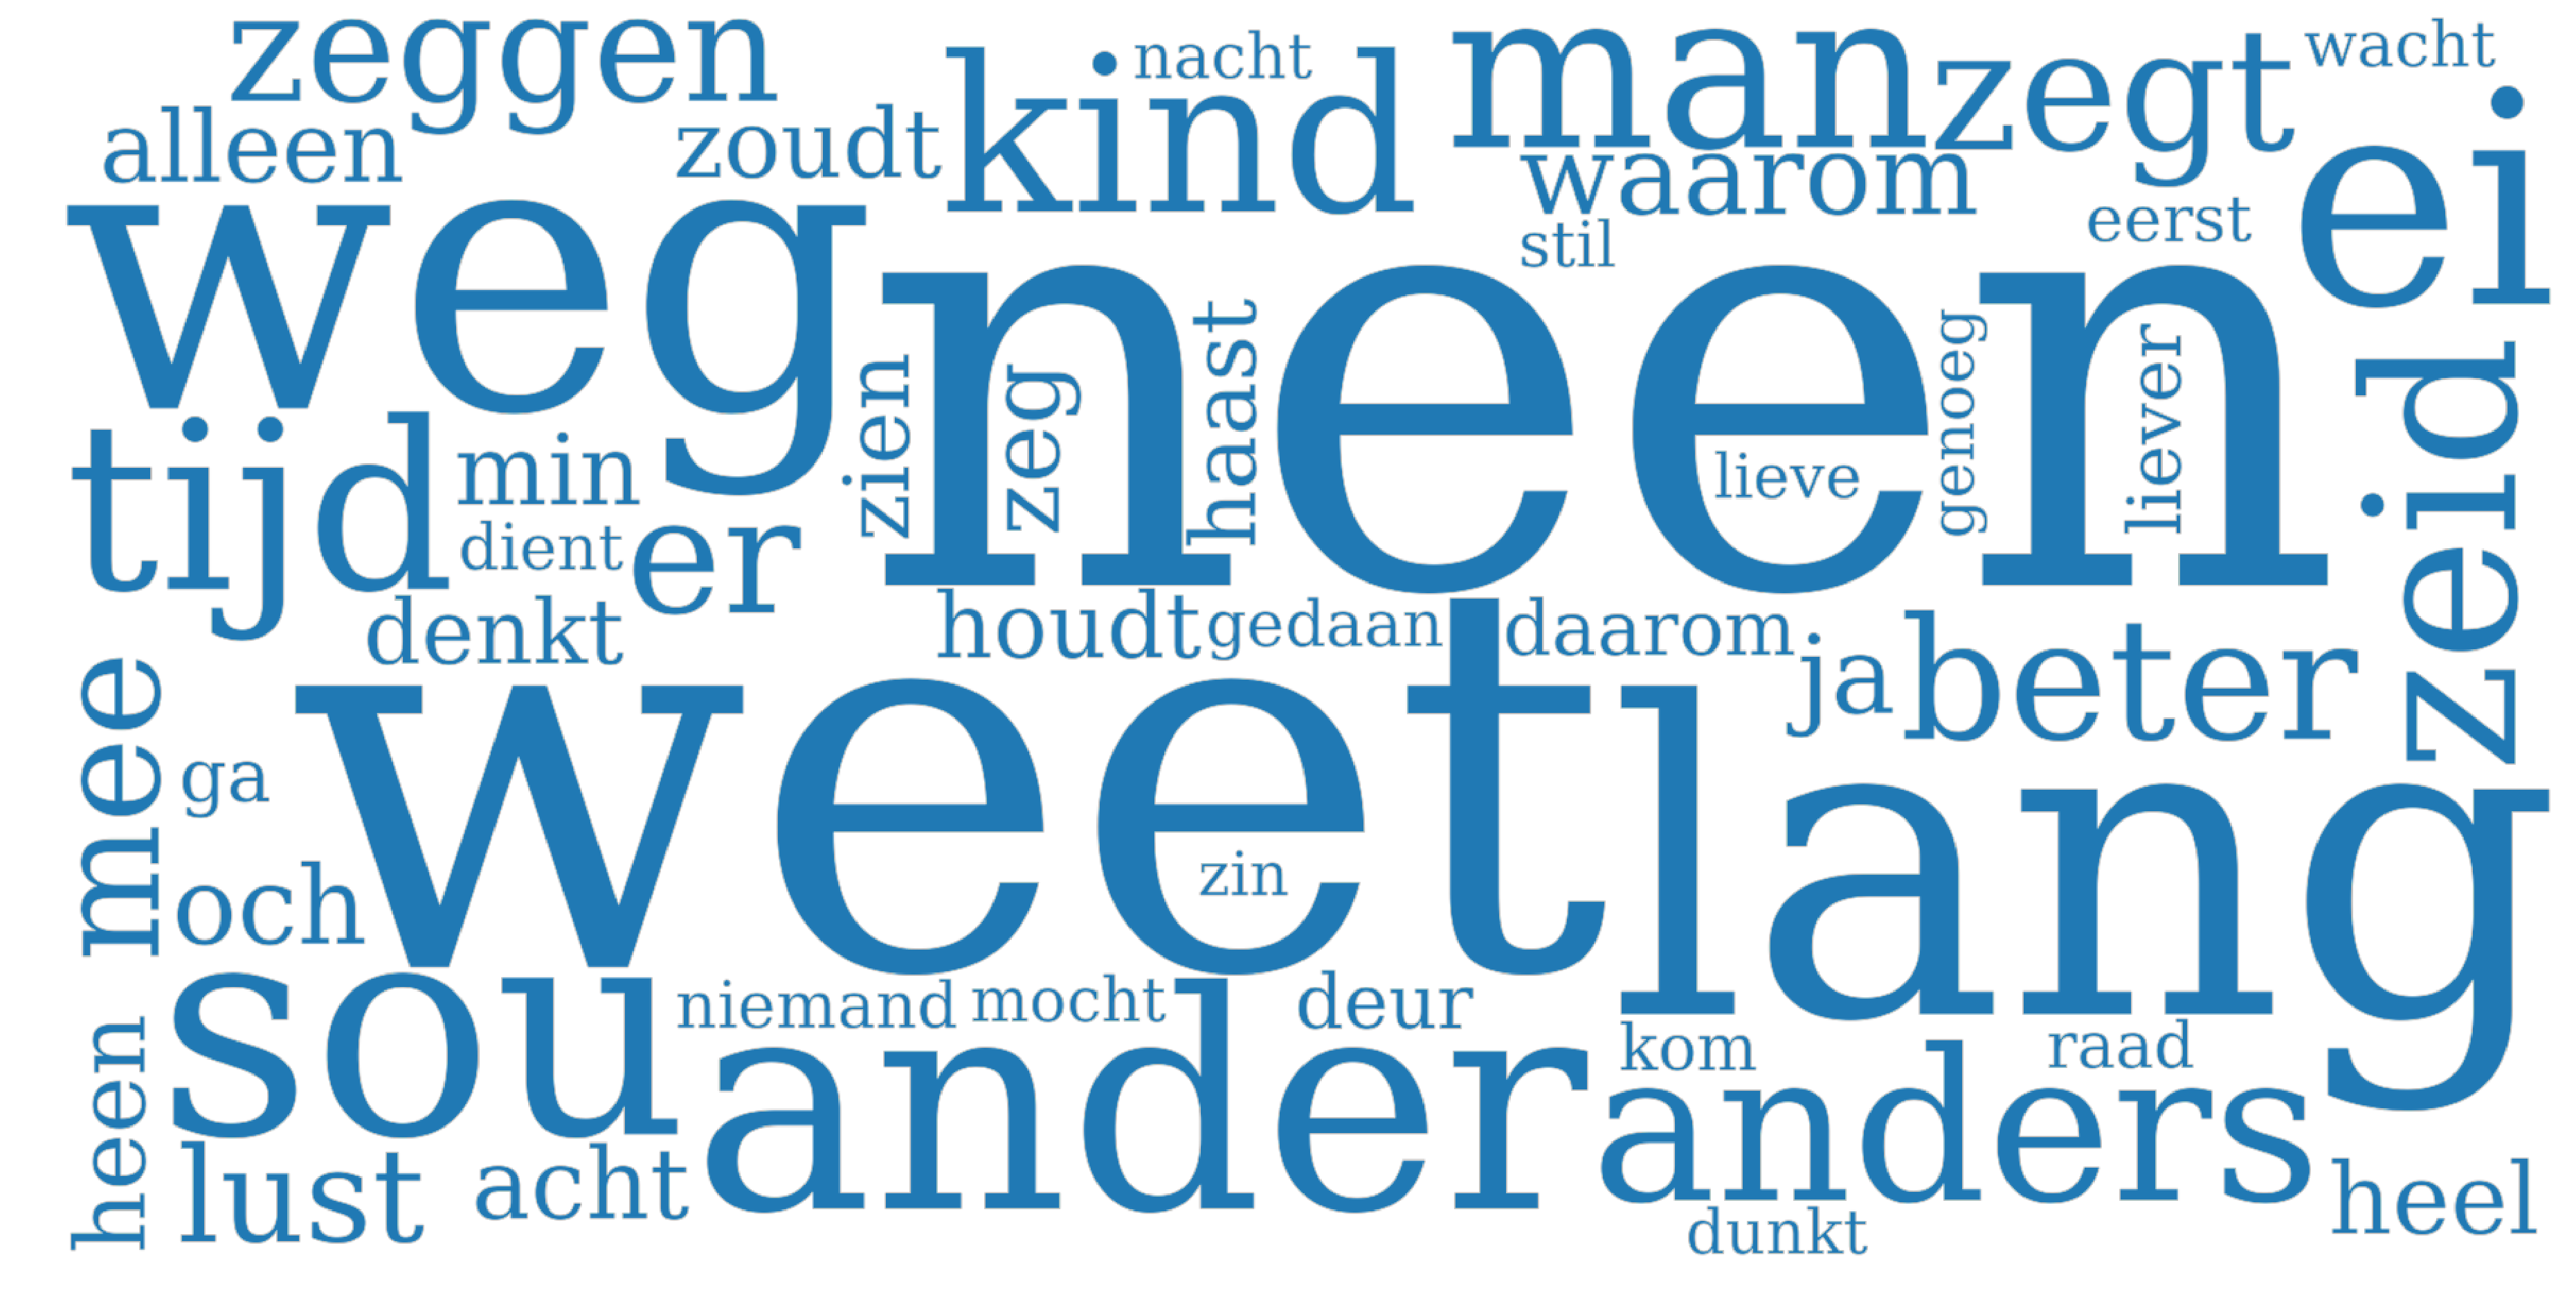
\includegraphics[width=\linewidth]{VARD2_topic24}
		\caption{\textit{rejection} (24, VARD2)}
		\label{fig:topic24VARD2}
		\vspace{4ex}
	\end{minipage}%%
	\begin{minipage}[c]{0.48\linewidth}
		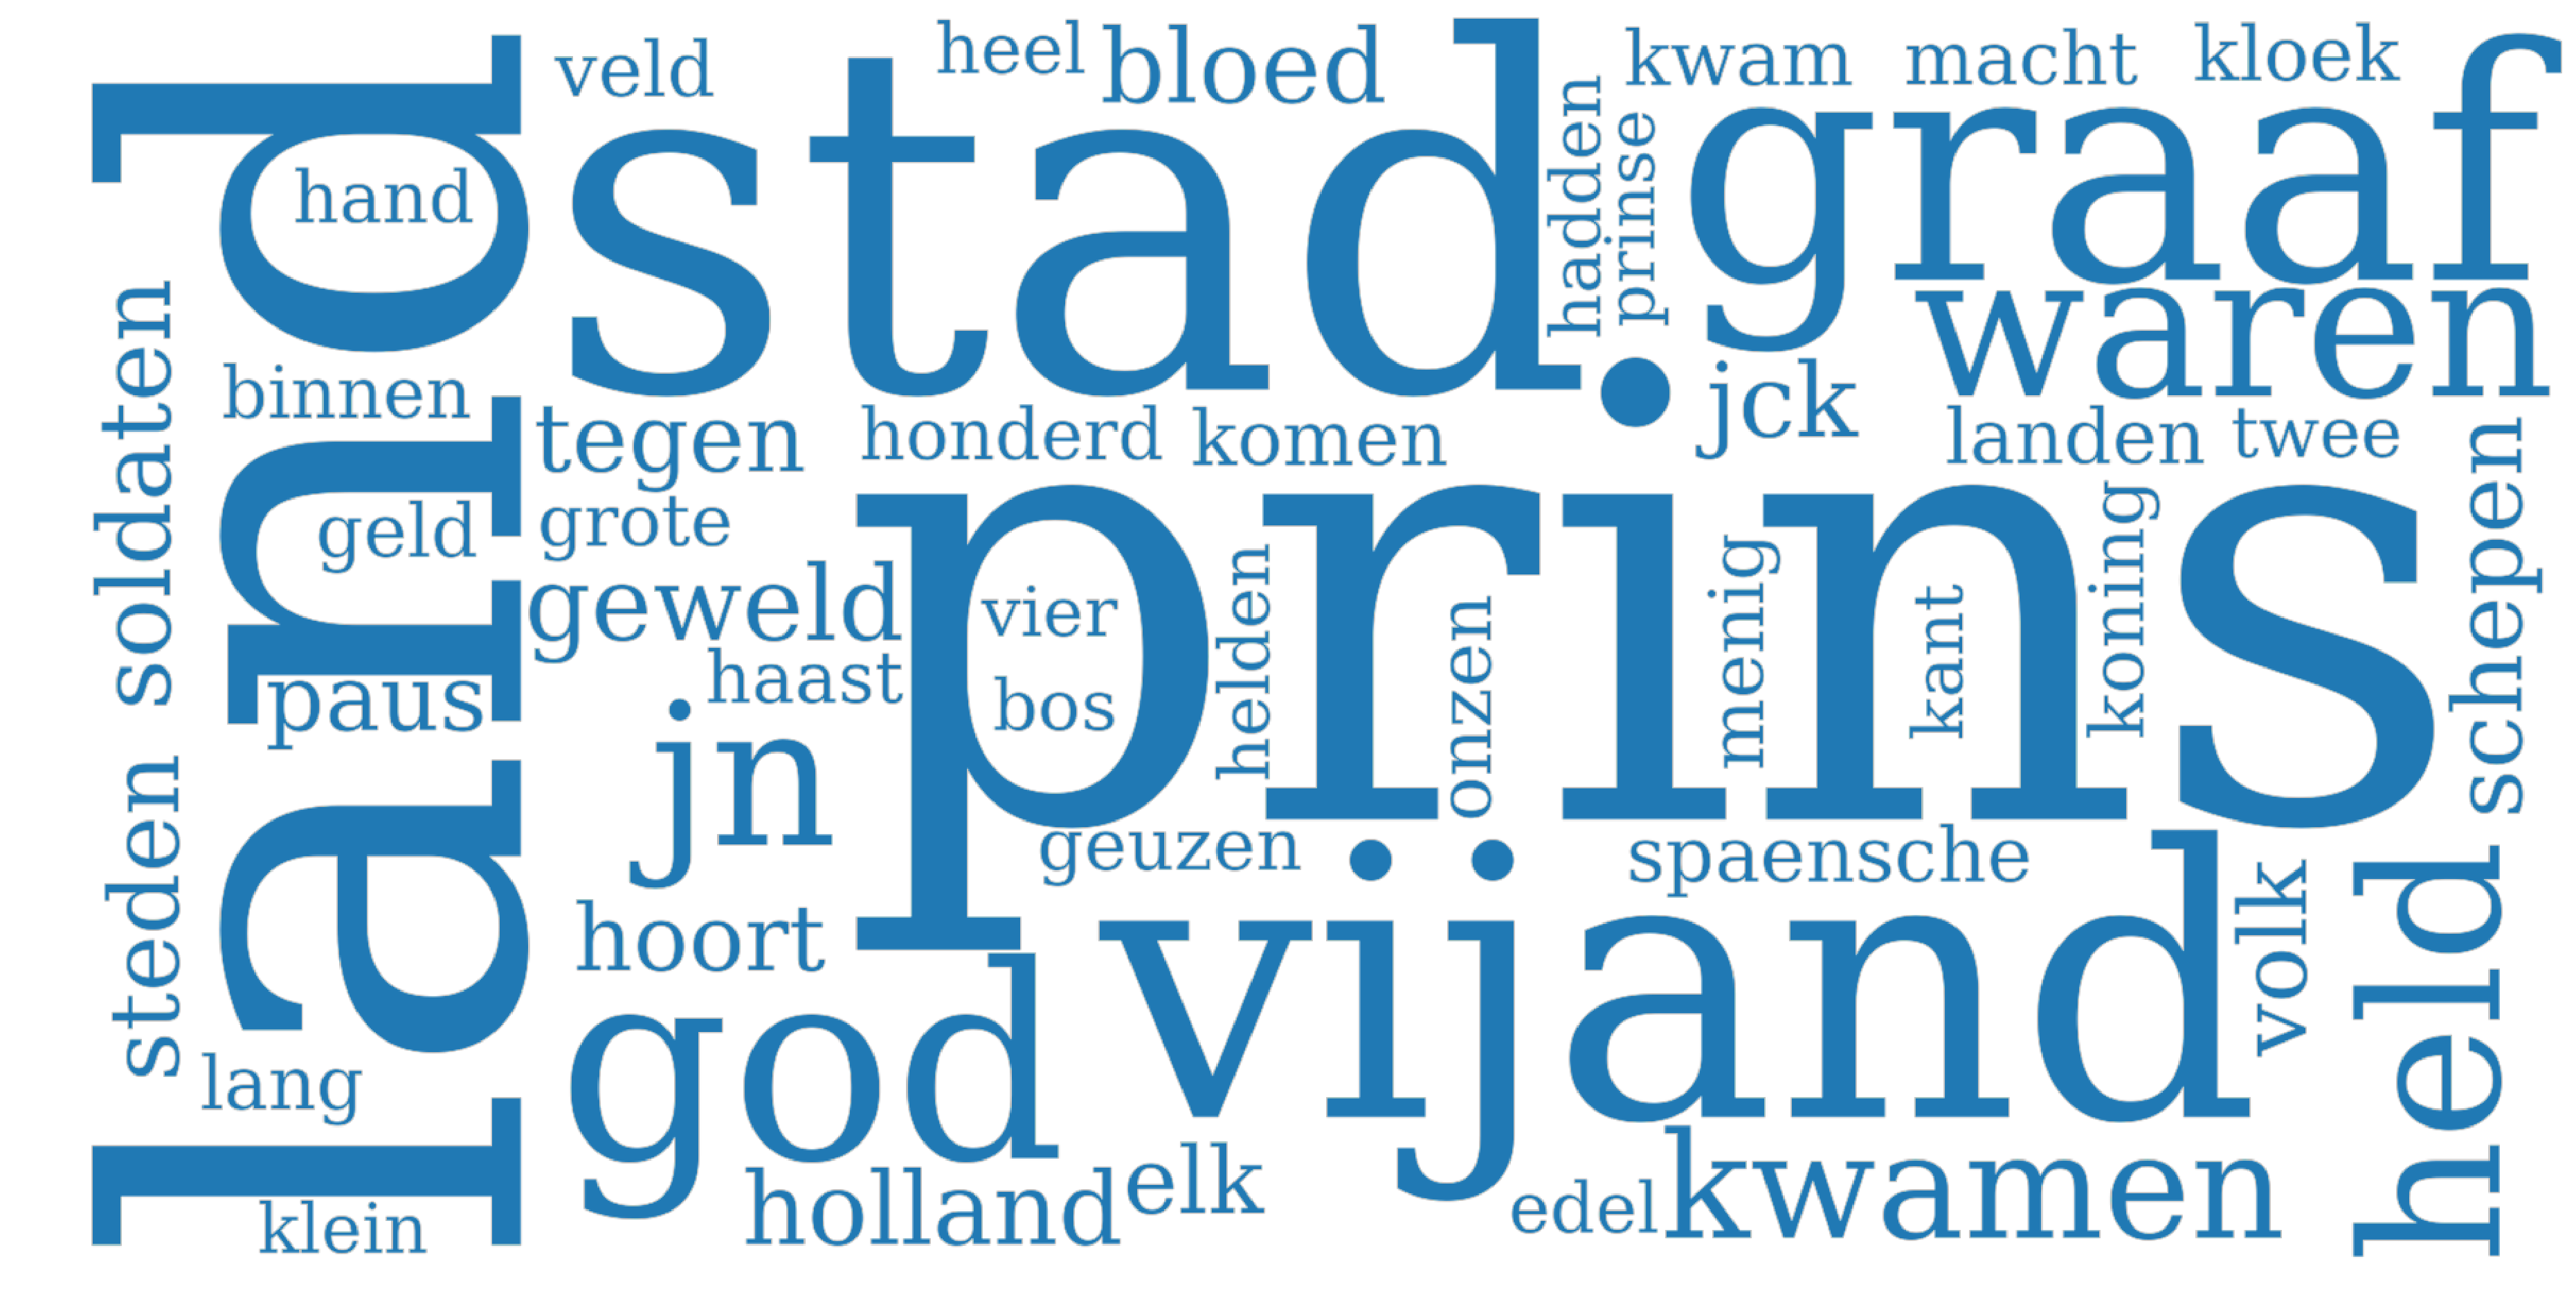
\includegraphics[width=\linewidth]{VARD2_topic32}
		\caption{\textit{nation \& country} (32, VARD2)}
		\label{fig:topic32VARD2}
		\vspace{4ex}
	\end{minipage}%%
\end{figure}

\noindent Geuzen songs were named after the Geuzen, the nickname for them who fought against the Spanish during the Dutch Revolt. In Geuzen songs, the motives for the battle against the Spanish were expressed, which is also the case in the song quoted above.

\section{Evaluating models}
Now that I have built three models from the three versions of my corpus, it is essential to evaluate the models and decide which one is the most worthwhile to continue my analysis with. It will come as no surprise anymore that the corpus normalized with the INL-tool is not worth the effort to investigate any further. Existing differences in words are smoothed out by wrong normalizations, resulting in inconclusive, resembling topics. The two remaining models are the one build from the original corpus, and the one build from the VARD2-normalized corpus. The biggest advantage of building topics from the original corpus, is that there is no risk in words losing their original meaning. However, this enormous word variation is at the same time a major disadvantage. The dictionary built from the original corpus is much larger than the dictionary from the VARD2-normalized corpus: 218,027 tokens versus 194,159 tokens. After discarding tokens that appear only one time, the difference is still considerable: 90,091 versus 77,114 tokens. This means that, when building topics from the original corpus, 12,977 words were considered as unique words, while, according to the VARD2-tool, these words were just variants of one of the other 77,114 words. From the  original corpus are therefore topics composed that are based on the time-specific spelling of the words. A negative consequence of this is that diachronic patterns in topical fluctuations are harder, or in fact impossible, to determine.

The VARD2-tool functions as a solution to that problem. The biggest advantage of this tool, compared to the INL-tool, is that I am able to verify which word was normalized to which word. VARD2 not only gives the normalized texts as .txt-output, but also every text as .xml-file, in which the performed normalizations are tagged. Moreover, a statistical file with data about how many words are normalized in each text, is created as well. Considering all this, I will continue my analysis with the version of the corpus that is normalized with the VARD2-tool. Although there are still a number of topics which can be considered as trash, the coherence of the words in these topics is the best I got.

It is now necessary to extend the corpus with the other songs containing the same \textit{incnormid}, resulting in a corpus of 43,772 songs, in which to every song the most dominant topic is assigned. I have used the following block of code for this:

\begin{lstlisting}
nlb = pd.read_csv("data/nlb.csv", sep=",")
nlb_timeset = nlb[(nlb["jaar_begin"] >= 1550) & (nlb["jaar_begin"] <= 1750)]
nlb_timeset = nlb_timeset[nlb_timeset["incnormid"] != 0] 

topics = pd.read_csv("VARD2_dominant_topic_per_song.csv", sep="\t", index_col=0)

msc = nlb_timeset.merge(topics, left_on="recordid", right_on="id")

nlb_timeset = nlb_timeset.loc[nlb_timeset["incnormid"].isin(msc["incnormid"])]

incs = msc.groupby("incnormid").first()[["dominant_topic", "perc_contribution"]]

topics = nlb_timeset.set_index("incnormid").join(incs).sort_values("incnormid")

topics = topics.reset_index()
\end{lstlisting}

\noindent The question is how the distribution of topics changes, now the size of the corpus almost has doubled. In Table~\ref{table:DomTopVARD2extended}, the new numbers of songs are presented. There are some changes in the ranking, but mostly because of religious topics that have taken over the Top10. A topic with a remarkable rise, is topic 32, on \textit{nation \& country}. Originally, there were 340 songs with this topic as the most prevalent one, but that number has increased to 1221. Earlier I showed that the song that represented this topic at best, was a Geuzen song. The expansion of this topic can be explained by the fact that song books with the so called Geuzen songs were reprinted a lot during the Dutch Revolt.

\begin{table}
	\begin{minipage}{0.5\textwidth}
		\begin{tabular}{ccl}
			\toprule
			Topic & Songs & Subject \\
			\midrule
			9              &            3936 & religion \& old spelling \\
			31             &            1966 & religion \\
			0              &            1848 & religion \& life \\
			28             &            1700 & intangible religion \\
			39             &            1671 & love \& sadness \\
			18             &            1631 & religion \\
			38             &            1607 & love \& happiness \\
			13             &            1403 & religion \\
			6              &            1277 & possessives \\
			32             &            1221 & nation \& country \\
			2              &            1073 & love \& tragedy \\
			24             &            1062 & rejection \\
			30             &            1038 & love \\
			1              &            1029 & religion \& Mary \\
			5              &            1021 & Christmas \\
			44             &             944 & religion \& virtue \\
			27             &             869 & world \& money \\
			12             &             841 & marriage \\
			47             &             787 & bucolic songs \\
			40             &             771 & religion \& Jesus \\
			48             &             767 & love \\
			8              &             755 & godly life \\
			46             &             752 & earthly life \\
			19             &             744 & verbs \\
			4              &             693 & religion \& happiness \\
			\vdots & \vdots & \vdots \\
			\bottomrule
		\end{tabular}
	\end{minipage}
	\begin{minipage}{0.5\textwidth}
		\begin{tabular}{|ccl}
			\toprule
			Topic & Songs & Subject \\
			\midrule
			\vdots & \vdots & \vdots \\
			36             &             686 & religion \\
			17             &             683 & heaven \\
			7              &             675 & God \& enemy \\
			14             &             655 & myth \& beauty \\
			49             &             646 & God \& country \\
			10             &             642 & suffer \& sadness \\
			34             &             628 & seducing \\
			21             &             625 & love \& happiness \\
			3              &             618 & verbs \\
			42             &             616 & cross \& passion \\
			23             &             602 & physical love \\
			29             &             590 & drinking \\
			16             &             572 & good \& evil \\
			15             &             546 & Old Testament \\
			37             &             501 & nature \\
			33             &             492 & ??? \\
			26             &             418 & money \& work \\
			35             &             410 & religion \\
			11             &             392 & entertainment \\
			22             &             329 & church \\
			25             &             312 & sea \\
			45             &             302 & trash \\
			41             &             170 & German \\
			43             &             148 & French\\
			20             &             108 & solfège\\
			\bottomrule
		\end{tabular}
	\end{minipage}
	\caption{Dominant topics in VARD2-normalized corpus (\textit{n} = 43,772)}
	\label{table:DomTopVARD2extended}
\end{table}

A methodical choice that needs some critical evaluation, is the fact that I picked the most dominant topic for each song and discarded the rest. It is possible, though, that a certain topic is very often the second-popular topic of a song. If that topic is rarely the most popular topic, it will end at the bottom of the ranking as stored in Tables~\ref{table:DomTopVARD2} and~\ref{table:DomTopVARD2extended}, although it can be a rather prevalent topic within the corpus. Another hypothesis, which can not be tested with the current method and the results arising therefrom, is that certain topics often occur together in a Top3 of topic contributions of a song. To get more insight in these trends, I extracted the Top3 topics of each song with the following code:

\begin{lstlisting}
transformed_docs = lda.load_document_topics()
docs = [[texts[indx]] + [p[1] for p in doc] for indx, doc in enumerate(transformed_docs)]
composition = pd.DataFrame(docs, columns=["document_id"] + ["topic {}".format(x) for x in range(0, N_TOPICS)])

arr = np.argsort(-composition.values, axis=1)
df1 = pd.DataFrame(composition.columns[arr], index=composition.index)

top3topics = df1[[0, 1, 2]].copy()
top3topics.columns = ["top1", "top2", "top3"]

songstop = nlb_timeset.merge(top3topics, left_on="recordid", right_on="id")
nlb_timeset = nlb_timeset.loc[nlb_timeset["incnormid"].isin
(songstop["incnormid"])]
incstop = songstop.groupby("incnormid").first()[["top1", "top2", "top3"]]

top3topicsong = nlb_timeset.set_index("incnormid").join(incstop).
sort_values("incnormid")
top3topicsong = top3topicsong.reset_index()
\end{lstlisting}

\noindent The result is a dataframe with 43,772 rows, where for each song (i.e. each row) the Top3 dominant topics are stored in columns. I grouped the topics that were in the second position of the Top3, and stored the most frequent ten of them in Table~\ref{table:SecondandThirdPopularTopics}. It turns out that from the Top10 second-popular topics, five topics were in the Top15 popular topics as well. They are all on religion.\footnote{Topics 31 (\textit{religion}), 9 (\textit{religion \& old spelling}), 18 (\textit{religion}), 0 (\textit{religion \& life}) and 24 (\textit{rejection}).} From the other five topic from the Top10 second-popular topics, two topics were composed of \textit{verbs}.\footnote{Topics 19 and 3.} The three other topics in the Top10 second-popular topics were on \textit{suffer \& sadness}, \textit{religion} and \textit{God \& enemy}. From the Top10 third-popular topics, eight topics were in the Top10 second-popular topics as well. The two \enquote{new} topics are topic 15 on the \textit{Old Testament} and topic 21 on \textit{love \& happiness}. I conclude therefore that, except the topics on \textit{God \& enemy} and the \textit{Old Testament}, the Top3 does not bring new topics to attention.

\begin{table}[]
	\centering
	\begin{tabular}{lll|lll}
		\toprule
		Topic 2 & Songs & Subject & Topic 3 & Songs & Subject  \\
		\midrule
		19 & 3456 & verbs 	&	19 &   4513 & verbs \\
		31 & 2295 & religion & 18  &  2244 & religion  \\
		9 & 2166 & religion \& old spelling & 10   & 1988 & suffer \& sadness\\
		18 & 2109 & religion & 0 & 1928 & religion \& life \\
		0 & 1724 & religion \& life & 3 & 1820 & verbs \\
		10 & 1693 & suffer \& sadness & 24 & 1790 & rejection \\
		24 & 1659 & rejection & 7 & 1659 & God \& enemy \\
		3 & 1658 & verbs & 36 & 1433 & religion \\
		36 & 1564 & religion & 15 & 1254 & Old Testament \\
		7 & 1342 & God \& enemy & 21 & 1235 & love \& happiness \\
		\bottomrule      
	\end{tabular}
	\caption{Top10 with second- and third-popular topics}
	\label{table:SecondandThirdPopularTopics}
\end{table}

The answer to my question what the most dominant topics in my corpus are, is \enquote{religion and something}, for sure. That result is not surprising at all: I already knew from the distribution of categories (Table~\ref{table:SongsCat}) that I could expect lots of topics concerning \enquote{religion}. However, since this category assigning has been in some cases quite general and arbitrary, the topic modeling method could give more insight in topical subdivisions within a genre. For some reason, LDA was able to distinguish songs that were merely on religion and happiness from songs that were merely on religion and virtue. The same applies to songs from the category \enquote{love and sex}. In the Dutch Song Database, thousands of songs are placed in this category, leaving no room for difference between songs on love and happiness, songs on love and sadness, or songs on rejection. Building a topic model has resulted in uncovering differences within the wide-ranging genres of songs. The next step I want to take in this thesis is how these topics in song lyrics fluctuate over time. Are songs on love and happiness and songs on love and sadness rising at the same time, or is the one a reaction to the other? When are songs on God and country becoming prevalent? Are there certain religious topics that disappear over time, being replaced by others? Can I indicate certain historical or cultural events that drive these trends? And how do my observations relate to prevailing theses in current research on the role of literature in the early modern centuries? Can I confirm that literature functions as a constructor of identity? Is the relation between politics and literature indeed reflected in my results? Does a certain ideology emerge from topics, and if so, which one? Are song topics becoming more and more variate over time, as well as the audience of songs? In the next chapter I will try to find an answer to these questions.




